
\documentclass[
  pagesize=pdftex,
  paper=letter,
  numbers=noenddot,
  %chapterprefix,
  %parskip=half,
  %fontsize=10.5pt,
  %twoside,
  BCOR=-12mm,
  DIV=9,
  %headings=openright,
  toc=listof,
  toc=bib,
  %draft
]{scrreprt}

\newcommand{\longtitle}{Deep Learning for Manifold Learning and Segmentation of
Brain MRIs}

%\usepackage[margin=3cm]{geometry}
\usepackage{ifthen}

% Charater sets, fonts and basics
\usepackage{fixltx2e}
\usepackage[latin1]{inputenc}
\usepackage[T1]{fontenc}

\usepackage[english]{babel}
\usepackage[english=british]{csquotes}

%\usepackage{lmodern}
\usepackage[sc, osf]{mathpazo}
\renewcommand*\sfdefault{uop}
\usepackage[scaled=.9]{luximono}
\linespread{1.10}
\usepackage{microtype}
\makeatletter
\def\MT@register@subst@font{\MT@exp@one@n\MT@in@clist\font@name\MT@font@list
   \ifMT@inlist@\else\xdef\MT@font@list{\MT@font@list\font@name,}\fi}
\makeatother 

% Math stuff
%\usepackage{dsfont,amsmath,amssymb,latexsym,soul}
\usepackage{amsmath,mathtools}
\usepackage{amsbsy,dsfont,soul,calc}
\DeclareMathOperator{\sinc}{sinc}
\DeclareMathOperator{\sigm}{sigm}
\DeclareMathOperator{\fft}{fft}
\DeclareMathOperator{\ifft}{ifft}
\sodef\so{}{.14em}{.4em plus.1em minus .1em}{.4em plus.1em minus .1em}

\usepackage[autokw]{svn-multi}
\svnid{$Id: preamble.tex 41 2012-08-01 17:29:41Z tbrosch $}

% Tikz
\usepackage{atbegshi}
\usepackage{tikz}
\usetikzlibrary{intersections,decorations.pathreplacing,fit,calc,positioning,shapes.geometric,matrix}
\tikzstyle{every node}+=[font=\sffamily\small]
\pgfdeclarelayer{background}
\pgfsetlayers{background,main}

%\usetikzlibrary{external}
%\tikzexternalize[prefix=tikzfigures/temp/] % activate
%\tikzset{external/export=false}
\newcommand{\tikzexternal}[2][false]{%
%\tikzset{external/export=true, external/remake next=#1}%
%\tikzsetnextfilename{#2}%
}

% Special Table hacks
\usepackage{array,booktabs,dcolumn,rotating,multirow,etoolbox}

\robustify\bfseries % requires etoolbox
\newcommand{\minitab}[2][l]{\begin{tabular}{#1}#2\end{tabular}}

\newcolumntype{d}[1]{%
>{\DC@{.}{.}{#1}}l<{\DC@end}%
}

\newcolumntype{.}{D{.}{.}{-1}}
\newcolumntype{L}[1]{>{\raggedright\arraybackslash}p{#1}}

%\usepackage[sf,SF]{subfigure}
\usepackage[font={sf,small},labelfont=md,subrefformat=parens]{subfig}

% Units
\usepackage{xfrac}
\usepackage[alsoload=binary]{siunitx}
\sisetup{
  seperr,
  %repeatunits=false,
  product-units = single,
  trapambigerr=false,
  trapambigrange=false,
  %tophrase={{ bis }},
  valuemode=math,
  unitmode=math,
  quotient-mode=fraction,
  fraction-function=\sfrac
}

\usepackage{tocstyle}
\newtocstyle[KOMAlike][leaders]{thesis}{
  %\settocfeature[-1]{dothook}{\bfseries}
  %\settocfeature[0]{dothook}{\bfseries}
}
\usetocstyle{thesis}

% Enumerates
\usepackage{paralist}

\usepackage{varioref}
\usepackage[
    pdftex,
	pdfpagemode=UseOutlines,
	pdfdisplaydoctitle=true,
	pdflang=en,
	pagebackref,
	bookmarksopen=true,
	bookmarksopenlevel={1}
]{hyperref}

% % Change Layout of Backref
\renewcommand*{\backref}[1]{%
  % default interface
  % #1: backref list
  %
  % We want to use the alternative interface,
  % therefore the definition is empty here.
}%
\renewcommand*{\backrefalt}[4]{%
  % alternative interface
  % #1: number of distinct back references
  % #2: backref list with distinct entries
  % #3: number of back references including duplicates
  % #4: backref list including duplicates
  \ifnum#1=0%
  \footnotesize\sffamily\color{red!50!gray}(not cited)%
  \else%
  \ifnum#1=1%
  \footnotesize\sffamily\color{gray}(cited on page~#2)%
  \else%
  \footnotesize\sffamily\color{gray}(cited on pages~#2)%
  \fi%
  \fi%
}

% Extraabstand fuer Fussnoten
\setlength{\skip\footins}{2em}

% Handle floats right
%\usepackage[above,below]{placeins}
%\usepackage{placeins}

\usepackage[version=3]{mhchem}

%\bibliographystyle{plain}
\usepackage{bibgerm}
\usepackage[sort]{natbib}
\bibliographystyle{gerapali}
%\bibliographystyle{gerplain}

% Listings
\usepackage{listings}

% Color definition
% Define special colors
\definecolor{listcomment}{rgb}{0.325,0.761,0.259}
\definecolor{listkeyword}{rgb}{0.243,0.306,0.408}
\definecolor{listnumbers}{gray}{0.65}
\definecolor{listlightgray}{gray}{0.955}
\definecolor{shadecolor}{named}{listlightgray}
\definecolor{stringcolor}{rgb}{0.341,0.243,0.416}

% Setup the listings environment
\lstset{
  frame = tb,
  framerule = 0.25pt,
  float,
  backgroundcolor={\color{listlightgray}},
  basicstyle = {\ttfamily\footnotesize},
  keywordstyle = {\ttfamily\color{listkeyword}\textbf},
  identifierstyle = {\ttfamily},
  commentstyle = {\ttfamily\color{listcomment}\textit},
  stringstyle = {\ttfamily\color{stringcolor}},
  showstringspaces = false,
  showtabs = false,
  numbers = left,
  numbersep = 6pt,
  numberstyle={\ttfamily\color{listnumbers}},
  tabsize = 2,
  language=C++,
  floatplacement=tb
  captionpos=b,
  escapeinside={<@}{@>},
  abovecaptionskip=7pt,
  morekeywords={__global__, __host__, __device__, uint, texture, float4, fmatrix4}
}

\usepackage[vlined,linesnumbered]{algorithm2e}
\SetNlSty{}{}{}
\SetArgSty{}
\DontPrintSemicolon

\usepackage[acronym,nonumberlist,toc,nomain]{glossaries}
\renewcommand*{\glspostdescription}{}
\setlength{\glsdescwidth}{0.7\textwidth}
\glossarystyle{super}
\renewcommand*{\glsgroupskip}{}

\AtBeginDocument{\labelformat{lstlisting}{Listing #1}}
\AtBeginDocument{\labelformat{chapter}{Chap\mbox{ter #1}}}
\AtBeginDocument{\labelformat{section}{Sec\mbox{tion #1}}}
\AtBeginDocument{\labelformat{subsection}{Sec\mbox{tion #1}}}
\AtBeginDocument{\labelformat{equation}{(#1)}}
\AtBeginDocument{\labelformat{table}{T\mbox{able #1}}}
\AtBeginDocument{\labelformat{figure}{F\mbox{igure #1}}}
\AtBeginDocument{\labelformat{Definition}{D\mbox{efinition #1}}}
%\AtBeginDocument{\labelformat{Satz}{Satz~#1}}
%\AtBeginDocument{\labelformat{Beispiel}{Beispiel~#1}}
%\AtBeginDocument{\labelformat{Beweis}{Beweis~#1}}

% Headings and footer
\usepackage{scrpage2}
\pagestyle{scrheadings}
\clearscrheadfoot
\ohead{\headmark}
\ofoot[\pagemark]{\pagemark}

\setheadsepline{.4pt}
\addtokomafont{pageheadfoot}{\normalfont\sffamily\small}
\addtokomafont{caption}{\sffamily\small}
\addtokomafont{captionlabel}{\sffamily\bfseries\small}
\addtokomafont{pagefoot}{\normalsize}
%\addtokomafont{chapter}{\glsresetall}
%\addtokomafont{page}{\normalsize}
%\automark[subsection]{section}
\automark{chapter}

%\addtokomafont{section}{
%{\tikzset{external/export=false}\tikz \fill[left color=primary-4,right color=white] (0,0) rectangle (\textwidth,1pt);}\\*}
\addtokomafont{dictumtext}{\normalfont\itshape}
\addtokomafont{dictumauthor}{\normalfont}

%\newcommand{\intro}[1]{\paragraph{Introduction}{\itshape #1}}
\newcommand{\intro}[1]{\noindent {\itshape #1}}
\newcommand{\question}[1]{\paragraph{Question}{\itshape #1}}
\newcommand{\answer}{\paragraph{Answer}}

\newcommand{\qa}[1]{\question{#1}\answer}


\usepackage[textwidth=3.3cm, textsize=footnotesize,
colorinlistoftodos, shadow]{todonotes}
\usepackage{textcomp,xspace}
\usepackage{dsfont,amsmath,amssymb,amsbsy}
\usepackage{setspace,comment}

\newcommand{\vect}[1]{\mathbf{#1}}
\newcommand{\R}{\ensuremath{\mathds{R}}}
\newcommand{\Q}{\ensuremath{\mathds{Q}}}
\newcommand{\N}{\ensuremath{\mathds{N}}}
\newcommand{\I}{\ensuremath{\mathds{I}}}
\newcommand{\E}{\ensuremath{\mathds{E}}}
\newcommand{\Z}{\ensuremath{\mathds{Z}}}
\newcommand{\D}{\ensuremath{\mathds{D}}}
\newcommand{\W}{\ensuremath{\mathds{W}}}
\newcommand{\B}{\ensuremath{\mathds{B}}}
\newcommand{\Sn}{\ensuremath{\mathds{S}}}

\newcommand{\thetas}{\boldsymbol{\theta}}
\newcommand{\deltas}{\boldsymbol{\delta}}
\newcommand{\data}{\mathcal{D}}
\newcommand{\Norm}{\ensuremath{\mathcal{N}}}
\newcommand{\given}{\mid}

% Define a counter for the inserted todonotes.
\newcounter{todoListItems}
\newcommand{\todoTrans}[2][ ]{%
	% Increment counter
	\addtocounter{todoListItems}{1}%
	\todo[%
		caption={\protect\hypertarget{todo\thetodoListItems}{}#2},
		#1]
	{
		\sffamily #2 \hfill
		\hyperlink{todo\thetodoListItems}{$\uparrow$}
	}
}

\newcommand{\addref}{\todoTrans[color=blue!40]{Needs reference.}\xspace}
\newcommand{\addcontent}[1]{\todoTrans[color=green!40, inline]{#1}\xspace}
\newcommand{\rewrite}[1]{\todoTrans[color=red!40]{#1}\xspace}
\newcommand{\clarify}[1]{\todoTrans[color=orange!40]{#1}\xspace}
\newcommand{\thoughts}[1]{\todoTrans[color=orange!40,
inline]{\textbf{Thoughts:} #1}\xspace}


\mathchardef\ordinarycolon\mathcode`\:
\mathcode`\:=\string"8000
\begingroup \catcode`\:=\active
  \gdef:{\mathrel{\mathop\ordinarycolon}}
\endgroup

\usepackage{datetime}

\newdateformat{thesisdate}{%
\monthname[\THEMONTH] \THEYEAR}

% Schuster jungen und hurenkinder
\clubpenalty = 10000
\widowpenalty = 10000
\displaywidowpenalty = 10000

\newcommand{\vs}{\emph{vs}\xspace}

\usepackage{typearea}
% \input{acronyms}

%\hypersetup{pdfsubject={\longtitle, Rev. \svnrev}}

%\svnid{$Id: proposal.tex 41 2012-08-01 17:29:41Z tbrosch $}

% \cfoot[\so{DRAFT}, rev.\,\svnrev---not for circulation]{\so{DRAFT},
% rev.\,\svnrev---not for circulation}

%water marks
%\usepackage{draftwatermark}
%\SetWatermarkLightness{0.95}


\title{\longtitle}
\author{Tom Brosch}

\begin{document}

\pagenumbering{roman}
%\svnid{$Id: titlepage.tex 43 2013-05-16 16:59:40Z tbrosch $}
\begin{titlepage}
\newlength{\smalltitlespace}
\newlength{\mediumtitlespace}
\newlength{\largetitlespace}
\setlength{\smalltitlespace}{1em}
\setlength{\mediumtitlespace}{1.5em}
\setlength{\largetitlespace}{3.5em}
\noindent
  \begin{center}
  \mbox{}\vfill
  \large\sffamily
  {\huge\bfseries\MakeUppercase{\longtitle}\\}\vspace{2em}
  by\\[1.5em]
  {\Large TOM BROSCH\\[\smalltitlespace]}
  {\Large Dipl.-Ing., Otto-von-Guericke-Universit\"at Magdeburg,
  2010\\[\largetitlespace]}
  {\Large A THESIS SUBMITTED IN PARTIAL
  FULFILLMENT OF\\
  THE REQUIREMENTS FOR THE DEGREE OF\\[\smalltitlespace]
  DOCTOR OF PHILOSOPHY\\[\smalltitlespace]}
  in\\[\smalltitlespace]
  {\Large THE FACULTY OF GRADUATE AND POSTDOCTORAL STUDIES\\[\smalltitlespace]
  (Biomedical Engineering)\\[\largetitlespace]}
  {\Large THE UNIVERSITY OF BRITISH COLUMBIA\\[\smalltitlespace]
  (Vancouver)\\[\largetitlespace]}
  \thesisdate\today\\[\smalltitlespace]
  {\rmfamily \textcopyright{}} Tom Brosch, 2015
  %\vfill
  \end{center}
\end{titlepage}
%\chapter*{Abstract}

\mbox{}\vspace{2em}
\begin{quotation}
\begin{center}
\textbf{Abstract}
\end{center}
\noindent
% The two main classes of medical image segmentation and classification methods,
% featured-based and model-based, both have inherent limitations. Feature-based
% methods rely on hand-crafted features, which requires good domain knowledge and
% do not adapt easily to different image domains. Model-based approaches rely on
% large amounts of carefully labelled data, which is time-consuming and laborious
% to acquire. On the other hand, large amounts of unlabelled images are widely
% available but none of the aforementioned methods are able to make good use of
% them. To overcome these limitations, I propose investigating self-taught
% learning for medical image segmentation and classification. Self-taught learning
% is a machine learning concept that describes the idea of using unlabelled and
% labelled samples to improve classification performance. Applied to medical image
% analysis, this means letting a machine learn the features that best represent
% images of a particular domain from unlabelled images and to use the learned
% domain-specific features for classification and segmentation. The classification
% task is therefore divided into two stages, the unsupervised feature learning
% stage and the supervised classification stage based on the learned features.
% Segmentation is treated as a classification problem at the pixel level. After
% mapping image features to pixel features, classification and segmentation are
% solved in the same way.

% The human brain has often served as a model for computer vision algorithms
% \citep{Lowe1999,Grigorescu2002}. But on the other hand, research suggests that
% visual processing algorithms encoded by the receptive field of neurons are
% learned from a continuous stream of images \citep{Wiesel1963} and refined later \citep{Karni1991}.
% Hence, instead of copying what the visual system has learned, a computer system
% should resemble the learning capabilities, so it can be tuned to different image
% domains and different classification and segmentation problems.
% Thereto, I propose to divide classification into \num{2} stages---the
% unsupervised feature learning stage and the supervised classification stage based on the
% learned features. Segmentation is treated as a classification problem at
% the pixel level. After mapping image features to pixel features, classification and
% segmentation are solved in the same way.
% 
% Motivated by the recent success in using convolutional deep belief networks
% (CDBNs) for unsupervised learning of image features \citep{Lee2009,Lee2011}, I
% have used a CDBN to learn hierarchical features of the corpus callosum.
% Higher level features resemble parts of the corpus callosum. For segmentation,
% they will potentially be useful to roughly localize the corpus callosum within a
% slice, while lower-level features can be used accurately segmentation the corpus
% callosum once if rough estimate is found. In the future, unsupervised and
% supervised machine learning techniques will be combined to develop trainable
% classification and segmentation algorithms for medical images that can easily
% adapt to different anatomical and pathological structures and different image
% modalities or combinations of different modalities using large sets of
% unlabelled images and only few labelled samples.

%  For example, SIFT features \citep{Lowe1999}, inspired by neurons of the
%  inferior temporal cortex, have proved to be very robust for object recognition.
%  Resembling the receptive field of simple cells of the primary visual cortex,
%  $2$D Gabor filters have been used to describe textures for
%  segmentation \citep{Grigorescu2002}.

% \Glspl{dbn} \citep{Hinton2006}, which have shown to be a good model of the
% learning processes of the brain, can be used to find patterns in or learn
% features from unlabelled data. In particular, \citet{Lee2007} have shown that a
% sparse kind of a DBN can learn features that resemble the receptive field of
% neurons of the visual areas V1 and V2 when trained on natural images.
% Automatically learned features by a DBN have been used to classify natural
% images, outperforming state-of-the-art methods for object category
% classification \citep{Lee2011}, recognition of handwritten digits
% \citep{Hinton2006a}, and facial expression recognition \citep{Larochelle2010}.
% However, to the best of my knowledge, DBNs have not yet been used to
% successfully classify or segment medical images.

% \citet{Raina2007} have denoted the idea of using unlabelled and labeled training
% data to improve classification performance as self-taught learning. They showed
% that using unlabelled images, the classification performance can be
% significantly increased when only few labelled training examples are available.
% Similar to transfer learning \citep{Pan2010}, self-taught learning does not
% require that samples from the labelled and unlabelled training set follow the
% same distribution. This is especially imported for classification and
% segmentation of medical images since the amount of labelled training data is
% often not sufficient to represent the large spectrum of anatomical and
% pathological variability.

% Even though self-taught learning using DBNs can be applied to find features in
% any kind of data in general, there are a few new challenges that need to be
% tackled when applied to medical images. First challenges are due to the larger
% size of medical images compared to images used in previous studies. In contrast
% to \num{392000} parameters when trained on \num{28x28} images
% \citep{Hinton2006a}, one layer of a DBN for midsagittal \gls{mri} slices of the
% brain with a resolution of \num{256x256} pixels would contain approximately
% \num{6.5e8} tunable parameters. Training of this model would require
% approximately \SI{9.6}{\giga\byte} of temporary memory just for storing the
% current set of parameters and its gradient.
% 
% \Glspl{cdbn} \citep{Lee2009,Lee2011} have been proposed, which dramatically
% reduce the number of tunable parameters at the cost of more computational
% expensive operations. \citet{Krizhevsky2010} reported a training time of
% \num{45} hours in a recent attempt to speed up the training of a CDBN on
% \num{32x32} pixel images by exploiting the computational power of GPUs.
% \citet{Lee2009,Lee2011} have shown that a CDBN can scale to images up to a
% resolution of \num{150x150} without reporting training times. One major part of
% my thesis will therefore be to optimize current training algorithms in order to
% make the training of full-resolution volumes feasible.
% 
% A second challenge is to make sure that the learned features are useful for
% classification and segmentation. Even though the learned features depend mostly
% on the training images, some general characteristics of the learned features can
% be influenced by adjusting the hyperparameters of the DBN (e.g. the number of
% neurons, the number of layers, sparsity target). \citet{Hinton_2010} and
% \citet{Lee2011} have provided some general guidance for setting these parameters
% mainly for the purpose of classifying natural images. Since differences between
% medical images are relatively small compared to the whole spectrum of natural
% images, features useful for medical image classification must also be able to
% capture more subtle differences. For segmentation, it has to be made sure that
% features are specific to certain regions in the brain in order to describe the
% location-dependent context. A second major part of my thesis will therefore be
% to design strategies that help to monitor features during learning and to
% develop appropriate learning strategies or heuristics to set the
% hyperparameters.

% It
% is expected that prior knowledge about the image domain learned from
% unlabelled images will help to increase the robustness and accuracy of the
% classification and segmentation algorithm. In the machine learning community,
% using unlabelled data to improve classification performance is referred to as self-taught
% learning. The goal of the thesis can therefore be rephrased to applying the
% principle of self-taught learning to medical image classification and
% segmentation.
% 
% A DBN will be used to model the learning processes required to implement
% self-taught learning. Therefore, more efficient training methods must be
% developed in order to unlock the potential of DBNs for medical image analysis.
% In the process of training a DBN on medical images, the thesis is expected to
% advance the knowledge of how DBNs behave when applied to $3$D images
% in general and to $3$D medical images in particular. A central
% research question will be how the filters learned by a $3$D CDBN
% will look like. It is expected that, analogous to the $2$D case, filters of the
% first layer will resemble $3$D edge detectors and $3$D Gabor
% filters.\clarify{It feels like I need one more sentence here.}
% 
% In order to guarantee that the learned features from the DBN are useful for
% classification and segmentation, the relationship between hyperparameters,
% learned features, and their impact on the classification and segmentation
% performance will be investigated. It is expected that the gained knowledge from
% the previous analysis will lead to a set of rules and heuristics that can be
% used to set the hyperparameters of a DBN.
% 
% In addition, the thesis will produce software for fully automatic segmentation
% and classification for medical images based on trainable models. As part of the
% evaluation, trained models will be created for the following
% segmentation and classification problems:
% \begin{inparaenum}[(a)]
%   \item segmentation of the corpus callosum using midsagittal MRI slices of the
%   brain,
%   \item segmentation of MS lesions using registered full-resolution T$2$ and
%   proton density weighted MRI scans,
%   \item segmentation of deep grey matter like the hippocampus using
%   full-resolution MRI scans,
%   \item segmentation of T$1$ black hole lesions using registered
%   T$1$ and T$2$ weighted MRI scans, and
%   \item classification of \gls{ms}, \gls{ad} and healthy subjects using
%   full-resolution MRI scans of the brain.
% \end{inparaenum}
\end{quotation}
\vfill
\noindent
\textbf{Brosch, Tom:}\\
\emph{\longtitle}\\
PhD thesis, The University of British Columbia, 2015
\doublespacing
\tableofcontents
\listoffigures
\printglossary[type=acronym,title=List of Abbreviations,toctitle=List of
Abbreviations]
\clearpage

\glsresetall
\pagenumbering{arabic}
\chapter{Introduction}

Introduction of deep learning and motivation. What is deep learning? Why is
everyone so hyped about it? What is the vision/promise? Thinking in feature
hierarchies. Neuroplasticity suggestions that this can be learned. Inspiration
for different models like neural networks. Old field but met with problems.
Renaissance with faster hardware, more data, layerwise pre-training. Latest
development is fast. Fill this with examples of different domains and how deep
learning helped to revolutionized object recognition, object detection, semantic
segmentation, speech recognition, natural language processing.

Goal of the thesis. What am I up to? If it was so successful in so many
different domain, can deep learning help to solve problems in the medical domain
and where can it have a big impact? In this thesis, we focus on two possible
applications of deep learning, unsupervised learning of features that are
descriptive of images as a whole. This is directly related to manifold learning
and learning the variability in brain MRIs and the relationship to diseases. The
other part is image segmentation with the focus on MS lesion segmentation.

% See literature review as a tool, not as a goal. Try to structure the thesis
% without it and put it where it belongs. Maybe restructure later. I needed a part
% of it already for the motivation. I will put a lot in it when I describe the
% methods. An I will put something in there, when I describe the applications.

Give an outlook. First introduce some deep learning methods. Then talk about
special challenges when it comes to 3D medical images. A big part is training.
Training in the frequency domain explained plus a discussion of related work. A
general introduction is followed by the applications of deep learning. This will
be a chapter on its own. Start with learning variability in images or global
image descriptors and then segmentation.

\section{Multiple Sclerosis}

Give some introduction to MS and why it is important and what the challenges are
and how that links to what I'm doing in this thesis.

\chapter{Background}

Background chapter on deep learning methods. Start with general introduction. I
want to talk about some deep learning methods. Main goal is learning a feature
hierarchy. Models are often biologically inspired. Neuroplasticity strong
motivator for learning. Start with either unsupervised or supervised models.
Explain what it means and why it is important. Unsupervised no need for labels,
which can be difficult to obtain. Supervised tuned to task. Can perform better
when enough labels are available. Requires careful regularization or lots of
data because more prone to overfitting.

% Reduce overlap with introduction)

% RBMs, DBNs, convRBMs, convDBNs for manifold learning and NN and CNN for lesion
% segmentation.

\section{Terminology}

\subsection{Unit Layers vs. Processing Layers}

The term layer can be confusing because different layers can be meant. One way
is to count the number of layers of units or just unit layers for short. The
transition from the input units to the output units involves one calculation.
Hence, an alternative way of counting layers is to count the number of
operations or processing layers. One processing layer takes the inputs of the
previous unit layers and transforms them to calculate the values of the output
unit layer. In the remainder, the term layer will refer to unit layer, and
processing layers will be named specifically.

\section{Learning from Labeled Data}

% If I put this first, I can argue with inspiration from biological models
% first.

\subsection{Neural Networks}

A dense neural network is a deterministic function that maps input data to the
desired outputs through the successive application of multiple nonlinear
mappings of the following form
\begin{align}
\vect{z}_l &= \vect{W}_l\vect{x}_{l-1} + \vect{b}_l, \\
\vect{x}_l &= f_l(\vect{z}_l),
\end{align}
where $\vect{x}_0$ denotes the input of the neural network, $\vect{x}_L$ denotes
the output, $L$ is the number of computational layers, $f_l$ are transfer
functions, $\vect{W}_l$ are weight matrices, and $\vect{b}_l$ are bias terms.
Popular choices for the transfer function are the sigmoid function $f(x) =
\sigm(x)$ and the rectified linear function $f(x) = \max(0, x)$. The same
transfer function is typically used for all layers except for the output layer.
The choice of the output transfer function depends on the learning task. For
classification, a 1-of-$n$ encoding of the output class is usually used in
combination with the softmax transfer function defined as
\begin{equation}
\text{softmax}(\vect{z})_i = \frac{\exp(z_i)}{\sum_{j=1}^n \exp(z_j)},
\end{equation}
where $\vect{z}$ denotes an $n$-dimensional output vector.

Given a training set $\data = \{(\vect{x}_0^{(i)}, \vect{y}^{(i)})\given i
\in [1, N] \}$, a neural network is trained by minimizing the error
between the predicted outputs $\vect{x}_L^{(i)}$ and the given labels
$\vect{y}^{(i)}$
\begin{equation}
\hat{\thetas} = \arg\min_{\thetas} \sum_{i = 1}^N E\Big(\vect{x}_L^{(i)},
\vect{y}^{(i)}\Big),
\end{equation}
where $\thetas$ denotes the trainable parameters of the neural network. Typical
choices for the error function are the sum of squared differences (SSD), and
cross-entropy.
The minimization problem can be solved using stochastic gradient descent (SGD)
\citep{Rumelhart1986,polyak1992}, which requires the calculation of the gradient
of the error function with respect to the model parameters. The gradient can be
calculated by backpropagation \citep{werbos1974} as follows
\begin{align}
\deltas_L &= \nabla_{\vect{x}_L}E \cdot f_L'(\vect{z}_L), \\
\deltas_l &= (\vect{W}_{l+1}^\text{T}\deltas_{l+1}) \cdot
f_l'(\vect{z}_l) & \text{for $l < L$,}\\
\nabla_{\vect{W}_l}E &= \deltas_l\vect{x}_{l-1}^\text{T}, \\
\nabla_{\vect{b}_l}E &= \deltas_l,
\end{align}
where $\nabla_{\vect{x}_L}E$ denotes the gradient of the error function with
respect to the predicted output and $\cdot$ denotes element-wise multiplication.

\subsection{Convolutional Neural Networks}

The structure of CNNs is inspired by the complex arrangement of simple and
complex cells found in the visual cortex \citep{hubel1962,hubel1968}. Simple
cells are only connected to a small sub-region of the previous layer and need to
be tiled to cover the entire visual field. In a CNN (see \ref{fig:cnn}),
simple cells are represented by convolutional layers, which exhibit a similar mechanism of local
connectivity and weight sharing. Complex cells combine the activation of simple
cells to add robustness to small translations. These cells are represented in
the form of pooling layers similar to the pooling layers found in convDBNs.
After several alternating convolutional and pooling layers, the activations of
the last convolutional layer are fed into one or more dense layers to
carry out the final classification.

\begin{figure}
\centering
\begin{tikzpicture}[%
scale=0.85,
x  = {(1cm,0cm)},
y  = {(0.33cm,0.23cm)},
z  = {(0cm,1cm)}
%z  = {(0.9cm,-0.1cm)},
%x  = {(0.33cm,0.23cm)},
%y  = {(0cm,1cm)}
]

\tikzstyle{every node}=[font=\small, inner sep=3pt, align=center]
\tikzstyle{every pin}=[align=center,fill=white]
\tikzstyle{dbnlabel}=[font=\sffamily\normalsize]

\tikzstyle{image}=[fill=white, fill opacity=0.75]
\tikzstyle{pinline}=[thin, black!35]
\tikzstyle{kernelline}=[very thin]


%%%%%%%%%%%%%%%%%         
% INPUT LAYER
%%%%%%%%%%%%%%%%%

\foreach \x in {1, ..., 3} {
\def\y{0.25*\x}
\draw[image] (\y, -2,-2) coordinate (A1\x) -- (\y, 2,-2)
coordinate (B1\x) -- (\y, 2,2) coordinate (C1\x) -- (\y, -2,2) -- cycle;

\draw[kernelline]
      (\y, -1.6, 1.6) \ifnum\x=3 \else -- +(0.25, 0, 0) +(0,0,0) \fi
   -- (\y, -0.8, 1.6) \ifnum\x=3 \else -- +(0.25, 0, 0) +(0,0,0) \fi
   -- (\y, -0.8, 0.8) \ifnum\x=3 \else -- +(0.25, 0, 0) +(0,0,0) \fi
   -- (\y, -1.6, 0.8) \ifnum\x=3 \else -- +(0.25, 0, 0) +(0,0,0) \fi
   -- (\y, -1.6, 1.6);
   ;
\ifnum\x=3
\draw[kernelline] (\y, -1.6, 1.6) coordinate(a1) -- (1.65, -1.2, 1.2);
\draw[kernelline] (\y, -1.6, 0.8) coordinate(b1) -- (1.65, -1.2, 1.2);
\draw[kernelline] (\y, -0.8, 0.8) coordinate(c1) -- (1.65, -1.2, 1.2);
\draw[kernelline] (\y, -0.8, 1.6) coordinate(d1) -- (1.65, -1.2, 1.2);
\fi
}

%%%%%%%%%%%%%%%%%         
% HIDDEN LAYER
%%%%%%%%%%%%%%%%%

\foreach \x in {0, ..., 7} {
\def\y{0.125*\x+1.65}
\draw[image] (\y,-1.6,-1.6) coordinate(A2\x) -- (\y,1.6,-1.6)
-- (\y,1.6,1.6) coordinate (C2\x) -- (\y,-1.6,1.6) coordinate(D2\x) -- cycle;

\draw[kernelline]
      (\y, -0.8, 0.8) \ifnum\x=7 \else -- +(0.125, 0, 0) +(0,0) \fi
   -- (\y, -0.4, 0.8) \ifnum\x=7 \else -- +(0.125, 0, 0) +(0,0) \fi
   -- (\y, -0.4, 0.4) \ifnum\x=7 \else -- +(0.125, 0, 0) +(0,0) \fi
   -- (\y, -0.8, 0.4) \ifnum\x=7 \else -- +(0.125, 0, 0) +(0,0) \fi
   -- (\y, -0.8, 0.8);
\ifnum\x=7
\draw[kernelline] (\y, -0.8, 0.8) coordinate(a2) -- (3.425, -0.6, 0.6);
\draw[kernelline] (\y, -0.8, 0.4) coordinate(b2) -- (3.425, -0.6, 0.6);
\draw[kernelline] (\y, -0.4, 0.4) coordinate(c2) -- (3.425, -0.6, 0.6);
\draw[kernelline] (\y, -0.4, 0.8) coordinate(d2) -- (3.425, -0.6, 0.6);
\fi 
}

\draw[decorate,decoration={brace,raise=20pt}] (A11|-C11) --node[above=25pt]
{Convolutional layer} (C27|-C11);

\foreach \x in {0, ..., 7} {
\def\y{0.125*\x+3.425}
\draw[image] (\y,-0.8,-0.8) coordinate(A3\x) -- (\y,0.8,-0.8)
-- (\y,0.8,0.8) coordinate (C3\x) -- (\y,-0.8,0.8) -- cycle;

\draw[kernelline]
      (\y, -0.6, +0.6) \ifnum\x=7 \else -- +(0.125, 0, 0) +(0,0) \fi
   -- (\y, +0.2, +0.6) \ifnum\x=7 \else -- +(0.125, 0, 0) +(0,0) \fi
   -- (\y, +0.2, -0.2) \ifnum\x=7 \else -- +(0.125, 0, 0) +(0,0) \fi
   -- (\y, -0.6, -0.2) \ifnum\x=7 \else -- +(0.125, 0, 0) +(0,0) \fi
   -- (\y, -0.6, +0.6);
\ifnum\x=7
\draw[kernelline] (\y, -0.6, +0.6) -- (5.2, -0.2, 0.2);
\draw[kernelline] (\y, -0.6, -0.2) -- (5.2, -0.2, 0.2);
\draw[kernelline] (\y, +0.2, -0.2) coordinate (g7) -- (5.2, -0.2, 0.2);
\draw[kernelline] (\y, +0.2, +0.6) -- (5.2, -0.2, 0.2);
\fi 
}

\draw[decorate,decoration={brace,raise=10pt}] (C21|-C21) --node[above=15pt]
{Pooling layer} (C37|-C21);

\foreach \x in {0, ..., 15} {
\def\y{0.125*\x+5.2}
\draw[image] (\y,-0.4,-0.4) coordinate (A4\x) -- (\y,0.4,-0.4)
-- (\y,0.4,0.4) coordinate (C4\x) -- (\y,-0.4,0.4) -- cycle;
}

\begin{scope}[xshift=9cm]
\foreach \x in {1,...,7} {
  \node[circle, draw] (v\x) at (0,0, 0.5*\x - 0.5*4) {};
}
\end{scope}

\draw[shorten >=10pt,shorten <=7pt,dashed] (A415-|C415)--(v1.south west);
\draw[shorten >=10pt,shorten <=7pt,dashed] (C415)--
node[label=120:Vectorize\\ hidden units] {} (v7.north west);

\begin{scope}[xshift=10.5cm]
%\foreach \x/\y in {1/-1.5, 2/-1, 3/-0.5, 4/0, 5/0.5, 6/1, 7/1.5} {
\foreach \x in {1,...,5} {
  \node[circle, draw] (h\x) at (0,0, 0.5*\x - 0.5*3) {};
}
\end{scope}

\foreach \x in {1,...,7} {
	\foreach \y in {1,...,5} {
		\draw (v\x)--(h\y);
	}
}

\draw[decorate,decoration={brace,raise=10pt}] (v7.west|-C21)
 --node[above=15pt] {Dense layer} (h1.east|-C21);
 
\node[above=15pt, fill=white,xshift=-25pt,inner sep=3pt, fill opacity=1, text
opacity=1] 
(convl) at (d1) {convolution};
\draw[pinline, shorten >=4pt, shorten <=2pt] (convl) -- (d1);

\node[above=15pt,fill=white,xshift=35pt,inner sep=3pt]
(pooll) at (d2) {pooling};
\draw[pinline, shorten >=4pt, shorten <=2pt] (pooll) -- (d2);

% Label units

\node[below=10pt,align=center] (input) at (A12) {Multimodal\\ input images};

\draw[pinline, shorten >=4pt] (input) -- (A11);
\draw[pinline, shorten >=4pt] (input) -- (A12);
\draw[pinline, shorten >=4pt] (input) -- (A13);

\node[below=40pt,xshift=20pt,inner sep=5pt] (hiddens) at (A31) {Hidden units};
\draw[pinline, shorten >=4pt] (hiddens) -- (A27);
\draw[pinline, shorten >=4pt] (hiddens) -- (A34);
\draw[pinline, shorten >=4pt] (hiddens) -- (A47);
\draw[pinline, shorten >=4pt] (hiddens) -- (v1);

\node[below=25pt,align=center] (output) at (h1) {Output\\ units};
\draw[pinline, shorten >=4pt] (output) -- (h1);

\begin{comment}

%%%%%%%%%%%%%%%%%         
% OUTPUT LAYER
%%%%%%%%%%%%%%%%%

\begin{scope}[canvas is xy plane at z=3.425]
\draw[image] (-2,-2) coordinate (A) -- (2,-2)
-- (2,2) coordinate (C) -- (-2,2) -- cycle;
\end{scope}

\node[xshift=-0.7cm, left] (lesion) at (A) {$S$};
\draw[pinline, shorten >=4pt] (lesion) -- (A);

\node[xshift=0.7cm, right] (y2) at (C) {$y^{(2)}$};
\draw[pinline, shorten <=4pt] (C) -- (y2);

\draw[decorate,decoration={brace,raise=75pt,mirror}] (B1-|C) --
node[right=80pt] {Convolutional\\ network} (G7-|C1);

\draw[decorate,decoration={brace,raise=95pt,mirror}] (G0-|C1) --
node[right=100pt] {Deconvolutional\\ network} (C);

\end{comment}

\end{tikzpicture}
\caption[Schematic illustration of a CNN]{Convolutional neural network with two
convolutional layers, one pooling layer and one dense layer. The activations of the last layer is the output of
the network.}
\label{fig:cnn}
\end{figure}

For multimodal 3D volumes, the neurons of convolutional and pooling layers are
arranged in a 4D lattice, where the first three dimensions correspond to the
dimensions of the input volume, and the forth dimension indexes
the input modality or channel. The activations of the output of a
convolutional layer are calculated by
\begin{equation}
x^{(l)}_j = f\Bigg(\sum_{i=1}^C\tilde{w}^{(l)}_{ij}*x^{(l-1)}_i
+ b^{(l)}_j\Bigg),
\end{equation}
where $l$ is the index of a convolutional layer, $x^{(l)}_j$ denotes the
$j$th channel of the output volume, $w^{(l)}_{ij}$ is a 3D filter
kernel connecting the $i$th channel of the input volume to the $j$th channel
of the output volume, and $b_j^{(l)}$ denotes the bias term of the $j$th output
channel. CNNs can be trained using stochastic gradient descent, where the
gradient can be derived analogously to dense neural networks and calculated using
backpropagation \citep{lecun1989,LeCun1998}. 

A major challenge for gradient-based optimization methods is the choice of an
appropriate learning rate. Classic stochastic gradient descent \citep{LeCun1998}
uses a fixed or decaying learning rate, which is the same for all parameters of
the model. However, the partial derivatives of parameters of different layers
can vary substantially in magnitude, which can require different learning rates.
In recent years, there has been an increasing interest in developing methods for
automatically choosing independent learning rates. Most methods (e.g., AdaGrad
\citep{duchi2011}, AdaDelta \citep{zeiler2012}, RMSprop \citep{dauphin2015}, and
Adam \citep{kingma2014}) collect different statistics of the partial derivatives
over multiple iterations and use this information to set an adaptive learning
rate for each parameter. This is especially important for the training of deep
networks, where the optimal learning rates often differ greatly for each layer.

% TODO: Also strided convolutional neural networks.

\subsection{Training and pre-training}

Problem with learning rate and stuff. Can be pre-trained.

\section{Learning from Unlabeled Data}

% More statistical learning and finding patterns of similarity.

One of the most important applications of deep learning is to learn a feature
hierarchy from unlabeled images. The key to learning such a hierarchy is the
ability of deep models to be trained layer by layer, where each layer acts as a
nonlinear feature extractor. Various methods have been proposed for feature
extraction from unlabeled images. In this section, we will first introduce the
restricted Boltzmann machines (RBMs) \citep{freund1992,hinton2010}, which are the
building blocks of deep belief networks (DBNs) \citep{Hinton2006b}, followed by
a short introduction to alternative feature extractors such as stacked denoising
autoencoders (SDAEs) \citep{vincent2010}.

% TODO: comparison to supervised methods similar to the introduction of the
% supervised methods section.

\subsection{From Restricted Boltzmann Machines to Deep Belief Networks}

% TODO: Illustrate with toy example.

An RBM is a probabilistic graphical models defined by a bipartite graph as shown
in Fig.~\ref{fig:rbm}. The units of the RBM are divided into two layers, one of
visible units $\vect{v}$ and the other of hidden units $\vect{h}$. There are no
direct connections between units within either layer. An RBM defines the joint
probability of visible and hidden units in terms of the energy $E$
\begin{align}
p(\vect{v}, \vect{h} \given \thetas) &=
\frac{1}{Z(\thetas)}e^{-E(\vect{v}, \vect{h} \given \thetas)}. \\
\intertext{When the visible and hidden units are binary, the energy is defined
as} 
-E(\vect{v}, \vect{h}\given \thetas) &= \sum_{i, j}v_i w_{ij} h_j +
\sum_i b_i v_i + \sum_j c_j h_j \\
&= \vect{v}^\textup{T}\vect{W}\vect{h} + \vect{b}^\textup{T}\vect{v} +
\vect{c}^\textup{T}\vect{h}
\end{align}
where $Z(\thetas)$ is a normalization constant, $\vect{W}$ denotes the weight
matrix that connects the visible units with the hidden units, $\vect{b}$ is a
vector containing the visible bias terms, $\vect{c}$ is a vector containing the
hidden bias terms, and $\thetas = \{\vect{W}, \vect{b}, \vect{c}\}$ are the
trainable parameters of the RBM.

\begin{figure}
\centering
\begin{tikzpicture}

\tikzstyle{gnode}=[shape=circle,draw=black]

\foreach \x in {1,...,3} {
  \node[gnode] (h\x) at (2*\x-4, 0) {$h_\x$};
}
\foreach \y in {1,...,5} {
  \node[gnode] (v\y) at (1.5*\y-4.5, -2) {$v_\y$};
}
\foreach \x in {1,...,3} {
  \foreach \y in {1,...,5} {
      \draw (h\x)--(v\y);
  }
}

\node[pin=120:$w_{11}$] at ($(v1)!.5!(h1)$) {};

\coordinate (rh) at (4,0);
\coordinate (rv) at (4,-2);

\node[fit=(v1)(v5)(rv),inner sep=0pt] (visibles) {};
\node[fit=(h1)(rh), inner sep=0pt] (hiddens) {};
\node[fit=(v1)(v3), inner xsep=0pt] (inputs) {};
\node[fit=(v4)(v5), inner xsep=0pt] (outputs) {};

\begin{scope}[decoration=brace]

\draw[decorate] ($(visibles.north east)-(0,2pt)$)--node[right=4pt]{Visible
units $\vect{v}$}
(visibles.south east);

\draw[decorate] (hiddens.north  east)--
node[right=4pt,align=center]{Hidden units $\vect{h}$}
($(hiddens.south east)+(0,2pt)$);

\draw[decorate] ($(hiddens.south east)-(0,2pt)$)
--node[right=4pt,align=left] {Weights $\vect{W}$ between\\ visibles and
hiddens} ($(visibles.north east)+(0,2pt)$);

% \draw[decorate] (inputs.south east)--
% node[below=4pt] {Input units: $\vect{x}$}
% (inputs.south west);
% \draw[decorate] (outputs.south east)--
% node[below=4pt] {Output units: $\vect{y}$}
% (outputs.south west);
\end{scope}

\end{tikzpicture}

\caption[Graph representation of an RBM with 3 hidden and 5 visible units]{%
Graph representation of an RBM with 3 hidden and 5 visible units.
An RBM models the joint probability of visible and hidden units. Edges between
vertices denote conditional dependence between the corresponding random
variables.}
  
\label{fig:rbm}
\end{figure}

\paragraph{Inference}
The hidden units represent patterns of similarity that can be observed in groups
of images. Once an RBM is trained, the features of a previously unseen image can
be extracted by calculating the expectation of the hidden units. The posterior
distribution of the hidden units given the visible units can be calculated by
\begin{equation}
\label{eq:dhgivenv}
p(h_j = 1 \given \vect{v}, \thetas) = \sigm(\vect{w}_{\cdot,j}^\text{T}\vect{v}
+ c_j),
\end{equation}
where $\vect{w}_{\cdot,j}$ denotes the $j$th column vector of $\vect{W}$, and
$\sigm(x)$ is the sigmoid function defined as $\sigm(x) = (1+ \exp(-x))^{-1}, x
\in \R$. An RBM is a generative model, which allows for the reconstruction of
an input signal given its features. This is achieved by calculating the expectation
of the visible units given the hidden units. The posterior distribution $p(v_i =
1 \given \vect{h}, \thetas)$ can be calculated by
\begin{equation}
\label{eq:dvgivenh}
p(v_i = 1 \given \vect{h}, \thetas) = \sigm(\vect{w}_{i,
\cdot}^\text{T}\vect{h} + b_i),
\end{equation}
where $\vect{w}_{i,\cdot}$ denotes the $i$th row vector of $\vect{W}$.
Reconstructing the visible units can be used to visualize the learned features.
To visualize the features associated with a particular hidden unit, all other
hidden units are set to zero and the expectation of the visible units is
calculated, which represents the pattern that causes a particular hidden
unit to be activated.

\paragraph{Training}

% \begin{itemize}
%   \item There are different training methods for RBMs.
%   \item Will focus on constrastive divergence.
%   \item Alternatives are stochastic bla with a reference
%   \item RBMs are trained using maximum likelihood estimation (MLE)
% \end{itemize}

RBMs can be trained by maximizing the likelihood or, more commonly, the log
likelihood of the training data, $\data = \{\vect{v}_n \given n \in [1, N] \}$,
which is called maximum likelihood estimation (MLE). The gradient of the log
likelihood function with respect to the weights, $\vect{W}$, is given by
\begin{equation}
\label{eq:mle}
\nabla_{\vect{W}} \log p(\mathcal{D} \given \thetas) =
\frac{1}{N} \sum_{n = 1}^N
\E[\vect{v}\vect{h}^\text{T} \given \vect{v}_n, \thetas]
-\E[\vect{v}\vect{h}^\text{T} \given \thetas].
\end{equation}
The first expectation can be estimated using a mean field approximation:
\begin{align}
\E[\vect{v}\vect{h}^\text{T} \given \vect{v}_n, \thetas] &\approx
\E[\vect{v} \given \vect{v}_n, \thetas]
\E[\vect{h}^\text{T} \given \vect{v}_n, \thetas], \\
&=\vect{v}_n\E[\vect{h}^\text{T} \given \vect{v}_n, \thetas].
\end{align}
The second expectation is typically estimated using a Monte Carlo
approximation
\begin{equation}
\E[\vect{v}\vect{h}^\text{T} \given \thetas] \approx
\frac{1}{S}\sum_{s=1}^{S}\vect{v}_s\vect{h}_s^\text{T},
\end{equation}
where $S$ is the number of generated samples, and $\vect{v}_s$ and $\vect{h}_s$
are samples drawn from $p(\vect{v}\given \thetas)$ and $p(\vect{h}\given
\thetas)$, respectively. Samples from an RBM can be generated efficiently using
block Gibbs sampling, in which the visible and hidden units are initialized
with random values and alternately sampled given the previous state using
\begin{align}
h_j &= \I(y_j < p(h_j = 1 \given \vect{v}, \thetas)) & \text{with $y_j \sim
\text{U}(0,1)$}\\
v_i &= \I(x_i < p(v_i \given \vect{h}, \thetas)) & \text{with $x_i \sim
\text{U}(0,1)$}
\end{align}
where $z \sim \text{U}(0,1)$ denotes a sample drawn from the uniform
distribution in the interval $[0,1]$ and $\I$~is the indicator function, which
is defined as $1$ if the argument is true and $0$ otherwise. After several
iterations, a sample generated by the Gibbs chain is distributed according to
$p(\vect{vh}\given \thetas)$.

If the Gibbs sampler is initialized at a data point from the training set and
only $1$ Monte Carlo sample is used to approximate the second expectation in
\eqref{eq:mle}, the learning algorithm is called contrastive divergence (CD)
\citep{hinton2002}. Alternatively, persistent CD (PCD) \citep{tieleman2008} uses
several separate Gibbs chains to generate data independent samples from the
model, which results in a better approximation of the gradient of the log
likelihood than CD. To speed up the training, the dataset is usually divided
into small subsets called mini-batches and a gradient step is performed for each
mini-batch. To avoid confusion with a gradient step, the term ``iteration'' is
generally avoided and the term ``epoch'' is used instead to indicate a sweep
through the entire dataset. Additional tricks to monitor and speed up the
training of an RBM can be found in Hinton's RBM training guide
\citep{hinton2010a}.

\paragraph{Deep belief networks}

A single RBM can be regarded as a nonlinear feature extractor. To learn a
hierarchical set of features, multiple RBMs are stacked and trained layer by
layer, where the first RBM is trained on the input data and subsequent RBMs are
trained on the hidden unit's activations computed from the previous RBM. The
stacking of RBMs can be repeated to initialize DBNs of any depth.

\paragraph{Alternative unit types}

To model real-valued inputs like the intensities of some medical images, the
binary visible units of an RBM are replaced with Gaussian visible units, which
leads to the following energy function
\begin{equation} 
-E(\vect{v}, \vect{h}\given \boldsymbol{\theta}) = \sum_{i,
j}\frac{v_i}{\sigma_i} w_{ij} h_j + \sum_i \frac{(v_i - b_i)^2}{2\sigma_i^2} +
\sum_j c_j h_j,
\end{equation}
where the mean of the $i$th visible unit is encoded in the bias term $b_i$,
and its standard deviation is given by $\sigma_i$. Although approaches have been
proposed to learn the standard deviation \citep{cho2011}, the
training data is often simply standardized to have zero mean and unit variance,
which yields to the following simplification for the inference of the visible
and hidden units:
\begin{align} 
\label{eq:ghgivenv}
\E[h_j \given \vect{v}, \thetas] &=
\sigm(\vect{w}_{\cdot,j}^\text{T}\vect{v} + c_j),\\
\label{eq:gvgivenh}
\E[v_i \given \vect{h}, \thetas] &= \vect{w}_{i,\cdot}^\text{T}\vect{h} +
b_i.
\end{align}

A binary hidden unit can only encode two states. In order to increase the
expressive power of the hidden units, Nair et al. proposed using noisy rectified
linear units (NReLU) \citep{nair2010} as the hidden units, and showed that this
can improve the learning performance of RBMs. The signal of an NReLU is the sum
of an infinite number of binary units all of which having the same weights but
different bias terms. In the special case where the offsets of their bias
terms are set to $-0.5, -1.5, \dotsc$, the sum of their probabilities and
therefore the expectation of an NReLU is extremely close to having a closed form:
\begin{align}
\E[h_j \given \vect{v}, \thetas] &=
\sum_{i=1}^\infty \sigm(\vect{w}_{\cdot,j}^\text{T}\vect{v} + c_j - i + 0.5),\\
&\approx \log(1+\exp(\vect{w}_{\cdot,j}^\text{T}\vect{v} + c_j)).
\end{align}
However, sampling of this type of unit involves the repeated calculation of the
sigmoid function, which can be time-consuming. If a sample is not constrained
to being an integer, a fast approximation can be calculated with
\begin{align} 
h_j &\sim \max(0, \mu_j + \Norm(0, \sigm(\mu_j))), \\
\mu_j &= \vect{w}_{\cdot,j}^\text{T}\vect{v} + c_j,
\end{align}
where $\Norm(0, \sigma^2)$ denotes Gaussian noise.

\subsection{Convolutional Models}

A potential drawback of DBNs is that the learned features are location
dependent. Hence, features that can occur at many different locations in an
image, such as edges and corners, have to be relearned for every possible
location, which dramatically increases the number of features required to
capture the content of large images. To increase the translational invariance of
the learned features, Lee et al. introduced the convolutional deep belief
network (convDBN) \citep{lee2009,lee2011}. In a convDBN, the units of one layer
are only connected to the units of a sub-region of the previous layer, where
each unit shares the same weights with all other units of the same layer. This
greatly reduces the number of trainable weights, which reduces the risk of
overfitting, reduces the memory required to store the model parameters, speeds
up the training, and thereby facilitates the application to high-resolution
images.

We assume the input images to be square 2D images, but the model generalizes
with little modification to non-square images of higher dimensions.

A convDBN consists of alternating convolutional and pooling layers, which are
followed by one or more dense layers. Each convolutional layer of the model can
be trained in a greedy layerwise fashion by treating it as a convolutional
restricted Boltzmann machine (convRBM). The energy of a convRBM is defined as
\begin{align} 
E(\vect{v},\vect{h}) 
% &= -\sum_{i=0}^{N_\text{c}-1} \sum_{j=0}^{N_\text{k}-1}
% \sum_{x,y=0}^{N_\text{h}-1} \sum_{u,v=0}^{N_\text{w}-1} h_{xy}^jw_{uv}^{ij}v_{x+u, y+v}^i
% - \sum_{i=0}^{N_\text{c}-1}b_i\!\sum_{x,y = 0}^{N_\text{v}-1}\!v_{xy}^i
% - \sum_{j=0}^{N_\text{k}-1}c_j\!\sum_{x,y = 0}^{N_\text{h}-1}\!h_{xy}^j \\
&= -\sum_{i=1}^{N_\text{c}} \sum_{j=1}^{N_\text{k}} \vect{h}^{(j)}
\bullet (\tilde{\vect{w}}^{(ij)} * \vect{v}^{(i)}) -
\sum_{i=1}^{N_\text{c}}b_i\sum_{x,y = 1}^{N_\text{v}}\!v_{xy}^{(i)} -
\sum_{j=1}^{N_\text{k}}c_j\sum_{x,y = 1}^{N_\text{h}}\!h_{xy}^{(j)}.
\end{align}
The key terms and notation are defined in Table~\ref{tab:notation}. At the first
layer, the number of channels $N_\text{c}$ is equal to the number of input
modalities. For subsequent layers, $N_\text{c}$ is equal to the number of
filters of the previous layer.

\begin{table} 
\caption{Key variables and notation. For notational simplicity,
we assume the input images to be square 2D images.}
\label{tab:notation}
\begin{center}
\begin{tabular}{@{}cL{10cm}@{}}
\toprule
Symbol & Description \\
\cmidrule(r){1-1}\cmidrule(l){2-2}
$\vect{v}^{(i)}$ & $i$th input channel \\
$\vect{h}^{(j)}$ & $j$th output channel or feature map \\
$\vect{w}^{(ij)}$ & weights of filter kernels connecting visible units
$\vect{v}^{(i)}$ to hidden units $\vect{h}^{(j)}$ \\
$b_i$ & bias terms of visible units \\
$c_j$ & bias terms of hidden units \\
$N_\text{c}$ & number of channels of the visible units \\
$N_\text{v}^2$ & number of visible units per channel \\
$N_\text{k}$ & number of filters and feature maps \\
$N_\text{h}^2$ & number of hidden units per feature map \\
%$N_\text{w}^2$ & number of weights per filter kernel \\
$\bullet$ & element-wise product followed by summation \\
$*$ & valid convolution \\
$\circledast$ & full convolution \\
$\tilde{\vect{w}}^{(ij)}$ & horizontally and vertically flipped version of
$\vect{w}^{(ij)}$ \\
\bottomrule
\end{tabular}
\end{center}
\end{table}
The posterior distributions $p(\vect{h} \given \vect{v})$ and $p(\vect{v} \given
\vect{h})$ can be derived from the energy equation and are given by
\begin{align}
p(h_{xy}^{(j)} = 1 \given \vect{v}) &= \sigm\Big(\sum_{i=0}^{N_\text{c}-1}
(\tilde{\vect{w}}^{(ij)}*\vect{v}^{(i)})_{xy} + c_j\Big), \\ 
p(v_{xy}^{(i)} = 1 \given \vect{h}) &= \sigm\Big(\sum_{j=0}^{N_\text{k}-1}
(\vect{w}^{(ij)} \circledast \vect{h}^{(j)})_{xy} + b_i\Big).
\end{align}
To train a convRBM on a set of images $\data = \{\vect{v}_n \given n \in
[1,N]\}$, the weights and bias terms can be learned by CD. During each iteration
of the algorithm, the gradient of each parameter is estimated and a gradient
step with a fixed learning rate is applied. The gradient of the filter weights
can be approximated by
\begin{equation}
\Delta \vect{w}^{(ij)} \approx
\frac{1}{N}(\vect{v}^{(i)}_n*\tilde{\vect{h}}^{(j)}_n -
\vect{v}'^{(i)}_n*\tilde{\vect{h}}_n'^{(j)}),
\label{eq:convgra}
\end{equation}
where $\vect{h}_n^{(j)}$ and $\vect{h}'^{(j)}_n$ are samples drawn from
$p(\vect{h}^{(j)} \given \vect{v}_n)$ and $p(\vect{h}^{(j)} \given
\vect{v}'_n)$, and $\vect{v}'^{(i)}_n = \E[\vect{v}^{(i)} \given \vect{h}_n]$.

Different types of operations \citep{scherer2010} have been
proposed for the pooling layers, with the common goal of creating a more compact
representation of the input data. The most commonly used type of pooling is
max-pooling. Therefore, the input to the pooling layer is divided into small
blocks and only the maximum value of each block as passed on to the next layer,
which makes the representation of the input invariant to small
translations in addition to reducing its dimensionality.

\subsection{Strided Convolutional Models}

% Why strided! Less memory, faster, no pooling required. Better correspondence
% to dense DBNs. Draw from the journal paper.

Strided convolutions are a type of convolution that shifts the filter kernel as
a sliding window with a step size or stride $s > 1$, stopping at only $N_\text{v}
/ s$ positions. This reduces the number of hidden units per channel to
$N_\text{h} = N_\text{v} / s$, hence significantly reducing training times and
memory required for storing the hidden units during training. The energy of a
strided convolutional RBM (sconvRBM) is defined as
\begin{equation} 
E(\vect{v},\vect{h}) = 
-\sum_{i=0}^{N_\text{c}-1}\sum_{j=0}^{N_\text{k}-1}\sum_{x,y=0}^{N_\text{h}-1}
\sum_{u,v=-\lfloor N_\text{w}/2\rfloor}^{\lfloor(N_\text{w}-1)/2\rfloor}
\hspace{-1.2em}h_{xy}^jw_{uv}^{ij}v_{sx+u, sy + v}^i -
\sum_{i=0}^{N_\text{c}-1}b_i\!\sum_{x,y = 0}^{N_\text{v}-1}\!v_{xy}^i -
\sum_{j=0}^{N_\text{k}-1}c_j\!\sum_{x,y = 0}^{N_\text{h}-1}\!h_{xy}^j
\end{equation}  

\subsection{Alternative Feature Learning Approaches}

Stacked auto encoders and denoising autoencoders without math. Independent
component analysis and independent subspace analysis. Need to read about this.

\chapter{Training on Medical Images: Training in the Frequency Domain}

Deep learning has traditionally been computationally expensive and advances in
training methods have been the prerequisite for expanding its application to a
variety of image classification problems. The development of layer-wise training
methods \citep{Hinton2006b} greatly improved the efficiency of the training of
deep belief networks (DBNs), which has made feasible the use of large sets of
small images (e.g. \num{28x28}), such as those used for hand-written digit
recognition. Subsequently, new directions for speeding up the training of deep
models were opened with the advance of programmable graphics cards (GPUs), which
can perform thousands of operations in parallel. \Citet{Raina2009} demonstrated
that by using graphics cards, training of restricted Boltzmann machines (RBMs)
on small image patches (e.g. \num{24x24}) can be performed up to \num{70} times
faster than on the CPU, facilitating the application to larger training sets.
However, the number of trainable weights of a DBN increases greatly with the
resolution of the training images, which can make training on large images
impracticable. In order to scale DBNs to high-resolution images,
\citet{lee2009,lee2011} introduced the convolutional deep belief network
(convDBN), a deep generative model that uses weight sharing to reduce the number
of trainable weights. They showed that a convDBN can be used to classify images
with a resolution up to \num{200x200} pixels. To speed up the training of
convolutional neural networks (CNNs) on high-resolution images,
\citet{Krizhevsky2012} replaced traditional convolutions of the first layer of
their CNN with strided convolutions, a type of convolution that shifts the
filter kernel as a sliding window with a fixed step size or stride greater than
one. Through the use of strided convolutions, the number of hidden units in each
convolutional layer is greatly reduced, which reduces both training time and
required memory. Using a highly optimized GPU implementation of convolutions,
they were able to train a CNN on images with a resolution of \num{256x256}
pixels, achieving state-of-the-art performance on the ILSVRC-2010 and
ILSVRC-2012 competitions \citep{Krizhevsky2012}. An alternative approach was
proposed by \citet{Mathieu2013} who sped up the training of CNNs by calculating
convolutions between batches of images and filters using fast Fourier transforms
(FFTs), albeit at the cost of additional memory required for storing the
filters.

In this paper, we detail our training algorithm and GPU implementation in full,
with a much more thorough analysis of the running time on high-resolution 2D
images (\num{512x512}) and 3D volumes (\num{128x128x128}), showing speed-ups of
up to 8-fold and 200-fold, respectively. Our proposed method performs training
in the frequency domain, which replaces the calculation of time-consuming
convolutions with simple element-wise multiplications, while adding only a small
number of FFTs. In contrast to similar FFT-based approaches
\citep[e.g.,][]{Mathieu2013}, our method does not use batch processing of the
images as a means to reduce the number of FFT calculations, but rather minimizes
FFTs even when processing a single image, which significantly reduces the
required amount of scarce GPU memory. We show that our method can be efficiently
implemented on multiple graphics cards, further improving the runtime
performance over other GPU-accelerated training methods. In addition, we
formalize the expression of the strided convolutional DBN (sconvDBN), a type of
convDBN that uses strided convolutions to speed up training and reduce memory
requirements, in terms of stride-1 convolutions, which enables the efficient
training of sconvDBNs in the frequency domain.

% TODO: Follow up with how to train them in the medical domain.
% Introduction and motivation. Talks about special challenges. Training in the
% frequency domain is important and a main contribution of this thesis. This will
% be about my algorithm, how it works for convRBMs and CNNs. Especially the tricks
% needed for strided convolutions.

\section{Algorithm}

% Mapping in the frequency domain. Minimize transforms. Also memory
% considerations and the likes. Also trick to do strided convolutions in the
% frequency domain.

\subsection{Training in the Spatial Domain}

% Short revision of how training works. Put all the pieces together to make it
% an algorithm. Make sure that I do this for convRBMs

To train an sconvRBM on a set of images, the
weights and bias terms can be learned by CD. During each iteration of the
algorithm, the gradient of each parameter is estimated and a gradient step with
a fixed learning rate is applied. The gradient of the filter weights can be
approximated by
\begin{equation}
\Delta \vect{W}^{ij} \approx \frac{1}{N}(\vect{V}^i_n*\tilde{\vect{h}}^j_n -
\vect{V}'^i_n*\tilde{\vect{h}}_n'^j)
\label{eq:convgra}
\end{equation}
where $\vect{V}_n, n \in [0,N-1]$ are reindexed images from the training set,
$\vect{h}_n^j$ and $\vect{h}'^j_n$ are samples drawn from $p(\vect{h}^j \given
\vect{V}_n)$ and $p(\vect{h}^j \given \vect{V}'_n)$, and $\vect{V}'^i_n =
\E[\vect{V}^i \given \vect{h}_n]$.
To apply the model to real-valued data like certain types of images, the
visible units can be modeled as Gaussian units. When the visible units are
mean--centered and standardized to unit variance, the expectation of the visible
units is given by
\begin{equation} 
\E[\vect{V}^i \given \vect{h}] = \textstyle\sum_j \vect{W}^{ij}*\vect{h}^j + b_i
\label{eq:convvis}
\end{equation}
A binary hidden unit can only encode two states. In order to increase the
expressive power of the hidden units, we use noisy rectified linear units as the
hidden units, which have been shown to improve the learning performance
of RBMs \citep{Nair2010}. The hidden units can be sampled with
\begin{align} 
\vect{h}^j &\sim \max(0, \mu^j + \Norm(0, \sigm(\mu^j))) \\
\mu^j &= \textstyle\sum_i\tilde{\vect{W}}^{ij}*\vect{V}^i +c_j
\label{eq:convhid}
\end{align} 
where $\Norm(0, \sigma^2)$ denotes Gaussian noise. The learning algorithm in the
spatial domain is summarized in Figure~\ref{alg:spatial}.

\begin{figure}[t!]
\hspace{-1.75em}
\subfloat[Training in the spatial domain]{
\label{alg:spatial}
\begin{minipage}{0.495\linewidth}
\footnotesize
\begin{algorithm}[H]
\setstretch{1.25}
%\renewcommand{\baselinestretch}{1.25}
%\selectfont
\SetKwInOut{Input}{input}
\SetKwInOut{Output}{output}
\Input{Images $\data = \{\vect{V}_n \given n \in [0, N-1]\}$}
\Output{Weights gradient $\Delta \vect{W}$}
$\Delta \vect{W} = 0$\;
\ForEach{image $\vect{V} \in \data$} {
  $\vect{V}' = 0$\;
  \For{$j = 0$ \KwTo $N_\text{k}-1$} {
    $\mu^j = \sum_i \tilde{\vect{W}^{ij}} * \vect{V}^i + c_j$\;
    \mbox{}\\
    \BlankLine
    $h^j \sim \max(0, \mu^j + \Norm(0, \sigm(\mu^j)))$\;
    \mbox{}\\
    \For{$i = 0$ \KwTo $N_\text{C}-1$} {
      $\Delta \vect{W}^{ij} = \Delta \vect{W}^{ij} + \tilde{\vect{h}}^j *
      \vect{V}^i$\;
      $\vect{V}'^i = \vect{V}'^i + \vect{W}^{ij} * \vect{h}^j$\;
    }
  }
  $\forall i \colon \vect{V}'^i = \vect{V}'^i + b_i$\;
  \For{$j = 0$ \KwTo $N_\text{k}-1$} {
    $\mu'^j = \sum_i \tilde{\vect{W}^{ij}} * \vect{V}'^i + c_j$\;
    \mbox{}\\
    $\vect{h}'^j \sim \max(0, \mu'^j +$\\ \hfill $\Norm(0, \sigm(\mu^j)))$\;
    \mbox{}\\
    \For{$i = 0$ \KwTo $N_\text{C}-1$} {
      $\Delta \vect{W}^{ij} = \Delta \vect{W}^{ij} - \tilde{\vect{h}}'^j *
      \vect{V}'^i$\;
    }
  }
}
\end{algorithm}
\end{minipage}
}
\subfloat[Training in the frequency domain]{
\label{alg:frequency}
\begin{minipage}{0.495\linewidth}
\footnotesize
\begin{algorithm}[H]
\setstretch{1.25}
%\renewcommand{\baselinestretch}{1.25}
%\selectfont
\SetKwInOut{Input}{input}
\SetKwInOut{Output}{output}
\Input{Images $\hat{\data} = \{\hat{\vect{V}}_n \given n \in [0, N-1]\}$}
\Output{Weights gradient $\Delta\hat{\vect{W}}$}
$\Delta\hat{\vect{W}} = 0$\;
\ForEach{image $\hat{\vect{V}} \in \hat{\data}$} {
  $\hat{\vect{V}}' = 0$\;
  \For{$j = 0$ \KwTo $N_\text{k} - 1$} {
    $\hat{\mu}^j = \sum_i \overline{\hat{\vect{W}}^{ij}} \cdot
    \hat{\vect{V}}^i$\; $\mu^j = \ifft(\hat{\mu}^j) + c_j$\;
    $\vect{h}^j \sim \max(0, \mu^j + \Norm(0, \sigm(\mu^j)))$\;
    $\hat{\vect{h}}^j = \fft(\vect{h}^j)$\;
    \For{$i = 0$ \KwTo $N_\text{C}-1$} {
      $\Delta\hat{\vect{W}}^{ij} = \Delta\hat{\vect{W}}^{ij} +
      \overline{\hat{\vect{h}}^j} \cdot \hat{\vect{V}}^i$\;
      $\hat{\vect{V}}'^i = \hat{\vect{V}}'^i + \hat{\vect{W}}^{ij} \cdot
      \hat{\vect{h}}^j$\;
    }
  }
  $\forall i \colon \hat{V}_{0,0}'^i = \hat{V}_{0,0}'^i +
  N_\text{V}^2b_i$\;
  \For{$j = 0$ \KwTo $N_\text{k}-1$} {
    $\hat{\mu}'^j = \sum_i \overline{\hat{\vect{W}}^{ij}} \cdot
    \hat{\vect{V}}'^i$\;
    $\mu'^j = \ifft(\hat{\mu}'^j) + c_j$\;
    $\vect{h}'^j \sim \max(0, \mu'^j +$ \\ \hfill $\Norm(0, \sigm(\mu^j)))$\;
    $\hat{\vect{h}}'^j = \fft(\vect{h}'^j)$\;
    \For{$i = 0$ \KwTo $N_\text{C}-1$} {
      $\Delta\hat{\vect{W}}^{ij} = \Delta\hat{\vect{W}}^{ij} -
      \overline{\hat{\vect{h}}'^j} \cdot \hat{\vect{V}}'^i$\;
    }
  }
}
\end{algorithm}
\end{minipage}
}
\caption{Comparison of training algorithms of convRBMs in (a) the
spatial and (b) the frequency domain. Training in the frequency domain replaces the
$5N_\text{k}N_\text{C}$ convolutions required in the spatial domain with simple
element-wise multiplications, while adding only $4N_\text{k}$ Fourier
transforms. The other operations are equivalent in both domains.}
\label{fig:algorithms}
\end{figure}

\subsection{Training in the Frequency Domain}

The computational bottleneck of the training algorithm in the spatial domain is
the calculation of convolutions, which needs to be performed $5 \times
N_\text{C} \times N_\text{k}$ times per iteration. To speed up the calculation
of convolutions, we perform training in the frequency domain, which maps the
convolutions to simple element-wise multiplications. This is especially
important for the training on 3D images due to the relatively large number of
weights of a 3D kernel compared to 2D. To minimize the number of Fourier
transforms, we map all operations needed for training to the frequency domain
whenever possible, which allows the training algorithm to stay almost entirely
in the frequency domain. All of the scalar operations needed for training
(multiplications and additions) can be readily mapped to the frequency domain
because the Fourier transform is a linear operation. Another necessary operation
is the flipping of a convolutional kernel $\tilde{w}(a) = w(-a)$, which can be
expressed by element-wise calculation of the complex conjugate; this follows
directly from the time-reversal property of the Fourier transform and the
reality condition $\hat{f}(-\xi)=\overline{\hat{f}(\xi)}$. Using the
aforementioned mappings, equations \eqref{eq:convgra} to \eqref{eq:convhid} can
be rewritten as
\begin{align}
\Delta \hat{\vect{W}}^{ij} &= \hat{\vect{V}}^i\cdot\overline{\hat{\vect{h}}^j}
- \hat{\vect{V}}'^i \cdot \overline{\hat{\vect{h}}'^j} \\
\E[\hat{V}_{xy}^i \given \vect{\hat{h}}] &=
\begin{dcases}
\textstyle\sum_j\hat{W}_{xy}^{ij}\hat{h}_{xy}^j + N_\text{V}^2 b_i &
\text{for } x,y = 0
\\
\textstyle\sum_j\hat{W}_{xy}^{ij}\hat{h}_{xy}^j & \text{for } x,y \neq 0
\end{dcases} \\
\hat{\vect{h}}^j &\sim \F\left(\max(0, \F^{-1}(\hat{\mu}^j) + c_j + 
\Norm(0, \sigma^2))\right) \\
\hat{\mu}^j
&=\textstyle\sum_i\overline{\hat{\vect{W}}^{ij}}\cdot\hat{\vect{V}}^i
\end{align}
where $\sigma^2 = \sigm(\F^{-1}(\hat{\mu}^j)+c_j)$, $\hat{x} = \F(x)$ denotes
$x$ in the frequency domain, $\F^{-1}$ denotes the inverse Fourier transform,
and $\cdot$ denotes element-wise multiplication. The algorithm for approximating the
gradient in the frequency domain is summarized in Figure~\ref{alg:frequency}.

The only operations that cannot be directly mapped to the frequency domain are
the calculation of the maximum function, the generation of Gaussian noise, and
trimming of the filter kernels. To perform the first two operations, an image
needs to be mapped to the spatial domain and back. However, these operations
need only be calculated $2N_\text{k}$ times per iteration and are therefore not
a significant contributor to the total running time. Because filter kernels are
padded to the input image size, the size of the learned filter kernels must be
explicitly enforced by trimming. This is done by transferring the filter kernels
to the spatial domain, setting the values outside of the specified filter kernel size
to zero, and then transforming the filter kernels back to the frequency domain.
This procedure needs to be performed only once per mini-batch. Since the number
of mini-batches is relatively small compared to the number of training images,
trimming of the filter kernels also does not add significantly to the total
running time of the training algorithm.

\subsection{GPU Implementation and Memory Considerations}

To further reduce training times, the algorithm can be efficiently implemented
on graphics cards, which can perform hundreds of operations in parallel.
To optimize efficiency, it is crucial to maximize the utilization of the large
number of available GPU cores, while minimizing the required amount of GPU
memory. Because our algorithm requires only a relatively small number of FFT
calculations per iteration, the computational bottleneck is the calculation of
the element-wise operations, which can be performed in parallel. Thus we
distribute the processing of a single 2D image over $N_\text{V}(\lfloor
N_\text{V}/2 \rfloor + 1) \times N_\text{C}$ independent threads, with one
thread per element in the frequency domain. The large number of parallel threads
results in a high utilization of the GPU, even when each image of a mini-batch
is processed sequentially, which we do in our method because this greatly
reduces the amount of GPU memory required to store the visible and hidden units
compared to processing batches of images in parallel.

Due to the relatively small amount of GPU memory compared to CPU memory, memory
requirements are an important consideration when designing a GPU algorithm.
However, the total amount of required memory is highly implementation-dependent
(e.g. the use of temporary variables for storing intermediate results) and a
comparison can only be done with common elements at the algorithmic level.
Therefore, in the remainder of this section, we focus on the memory requirements
of key variables such as the visible units, the hidden units, and the filters,
which are required by all implementations. In our training algorithm, all key
variables are stored in the frequency domain, where each element in the
frequency domain is represented by a single-precision complex number. Due to the
symmetry of the Fourier space, the number of elements that need to be stored is
roughly half the number of elements in the spatial domain. Thus, the memory
required for storing the visible and hidden units in the frequency domain is
roughly the same as in the spatial domain. A potential drawback of training in
the frequency domain is that the filters need to be padded to the size of the
visible units before applying the Fourier transformation, which increases the
memory required for storing the filters on the GPU. The total amount of memory
in bytes required for storing the visible units, hidden units, and padded
filters is given by the sum of their respective terms
\begin{equation} 
%\text{memory}_{\text{freq}} &= 8N_\text{v}(\lfloor N_\text{v}/2 \rfloor +1)
%\times (N_\text{c} + N_\text{k} + N_\text{k}N_\text{c}) \\
%&\approx 4N_\text{v}^2 \times (N_\text{c} + N_\text{k} + N_\text{k}N_\text{c})
% \\
% &\approx 
4N_\text{v}^2N_\text{c} + \frac{4N_\text{v}^2 N_\text{k}}{s^2} +
4N_\text{v}^2N_\text{k}N_\text{c}
\end{equation}
As a comparison, the training method of \cite{Krizhevsky2012} processes batches
of images in order to fully utilize the GPU, which requires the storing of
batches of visible and hidden units. The memory needed for storing the key
variables is given by
\begin{equation} 
%\text{memory}_{\text{spat}}= 4N_\text{v}^2 \times (N_\text{b}N_\text{c} +
% N_\text{b}N_\text{k}) + 4N_\text{w}^2N_\text{k}N_\text{c}
4N_\text{v}^2 N_\text{b}N_\text{c} + \frac{4N_\text{v}^2
N_\text{b}N_\text{k}}{s^2} + 4N_\text{w}^2N_\text{k}N_\text{c}
\end{equation}
where $N_\text{b}$ is the number of images per mini-batch. Depending on the
choice of the batch size, this method requires more memory for storing the
visible and hidden units, while requiring less memory for storing the filters.
Alternatively, \citet{Mathieu2013} proposed to speed up the training of CNNs by
calculating convolutions between batches of images and filters using FFTs. The
memory required for storing the visible units, hidden units, and filters using
this method is given by
\begin{equation}
%\text{memory}_{\text{freq}} &= 8 N_\text{v}(\lfloor N_\text{v}/2 \rfloor +1)
%\times (N_\text{b}N_\text{c} + N_\text{b}N_\text{k} + N_\text{k}N_\text{c}) \\
%&\approx 
4 N_\text{v}^2 N_\text{b}N_\text{c} + 4
N_\text{v}^2 N_\text{b}N_\text{k} + 4 N_\text{v}^2 N_\text{k}N_\text{c}
\end{equation}
Table~\ref{tab:memory} shows a comparison of the memory per GPU required for
storing key variables when training a network used in previous work by
\citet{Krizhevsky2012}. For the first layer, a comparison with Mathieu et al.'s
training method could not be performed, because that method does not support
strided convolutions, which would significantly reduce the memory required for
storing the hidden units. In all layers, the proposed approach compensates for
the increased memory requirements for the filters by considering one image at a
time rather than a batch, and still outperforms batched learning in the spatial
domain in terms of speed (see Section 3), despite not using batches.

% In all layers, the additional memory required for
% storing the padded filters is smaller than the memory required for storing
% batches of visible and hidden units. Thus, our method requires less memory for
% storing the key variables during training than two state-of-the-art
% GPU-accelerated methods.

\begin{table}[tb]
\caption{Comparison of the memory required for storing key
variables using different training methods: our method (Freq), Krizhevsky et al.'s spatial
domain method (Spat), and Mathieu et al.'s method using batched FFTs (B-FFT). A
comparison with Mathieu et al.'s method could not be made for the first layer,
because that method does not support strided convolutions. In all layers, our
method consumes less memory for storing the key variables than the other two
methods.}

\label{tab:memory}
\vspace{1em}
\centering

\sisetup{
  round-mode = places,
  round-precision = 1,
  exponent-product = \cdot,
  detect-weight=true,
  detect-inline-weight=math,
  tight-spacing = false,
  table-align-text-post = false
}%
\begin{tabular}{l
S[table-format=3.0]
S[table-format=3.0]
S[table-format=3.0]
S[table-format=2.0]
S[table-format=3.0]
S[table-format=1.0]
S[table-format=2.1]
S[table-format=3.1]
S[table-format=3.1]}
\toprule
Layer & {$N_\text{b}$} & {$N_\text{v}$} & {$N_\text{c}$} & {$N_\text{w}$} &
{$N_\text{k}$} & {$s$} & \multicolumn{3}{c}{Memory in MB} \\
& & & & & & & {Freq} & {Spat} & {B-FFT}
%{Out Method} & {\citet{Krizhevsky2012}} & {\cite{Mathieu2013}}
\\
\midrule
%1 (without striding) & 128 & 224 & 3 & 11 & 48 & 4 & 37.32422 & 1249.566 &
%1277.062 \\
1 & 128 & 224 & 3 & 11 & 48 & 4 & 28.71094 & 147.0665 & {---} \\
2 & 128 & 55 & 48 & 5 & 128 & 1 & 72.92938 & 260.5469 & 330.8594 \\
3 & 128 & 27 & 128 & 3 & 192 & 1 & 69.23364 & 114.75 & 182.25 \\
4 & 128 & 13 & 192 & 3 & 192 & 1 & 24.01318 & 32.95312 & 55.45312 \\
5 & 128 & 13 & 192 & 3 & 128 & 1 & 16.05005 & 27.25 & 42.25 \\
%\addlinespace
%Total & & & & & & & 210.9372 & 582.5665 & 330.8594 \\
\bottomrule
\end{tabular}\\[0.2em]
\end{table}

\subsection{Mapping Strided Convolutional to Stride-1 Convolutions}

Strided convolutions are a type of convolution that shifts the filter kernel as
a sliding window with a step size or stride $s > 1$, stopping at only $N_\text{v}
/ s$ positions. This reduces the number of hidden units per channel to
$N_\text{h} = N_\text{v} / s$, hence significantly reducing training times and
memory required for storing the hidden units during training. The energy of a
strided convolutional RBM (sconvRBM) is defined as
\begin{equation} 
E(\vect{v},\vect{h}) = 
-\sum_{i=0}^{N_\text{c}-1}\sum_{j=0}^{N_\text{k}-1}\sum_{x,y=0}^{N_\text{h}-1}
\sum_{u,v=-\lfloor N_\text{w}/2\rfloor}^{\lfloor(N_\text{w}-1)/2\rfloor}
\hspace{-1.2em}h_{xy}^jw_{uv}^{ij}v_{sx+u, sy + v}^i -
\sum_{i=0}^{N_\text{c}-1}b_i\!\sum_{x,y = 0}^{N_\text{v}-1}\!v_{xy}^i -
\sum_{j=0}^{N_\text{k}-1}c_j\!\sum_{x,y = 0}^{N_\text{h}-1}\!h_{xy}^j
\end{equation}  

\begin{figure}[tb]
\centering
\begin{tikzpicture}[node distance=0.9cm and 4.5cm]

\tikzstyle{every node}+=[font=\scriptsize\sffamily]
\tikzstyle{label}=[font=\footnotesize\sffamily]
\tikzstyle{lines}=[dashed,opacity=0]
\tikzstyle{mymatrix}=[%
  matrix of nodes,%
  inner sep=0pt,
  nodes={inner sep=2pt},
  %draw,%
  left delimiter  = (,%
  right delimiter = )%
]

\tikzstyle{every pin}+=[inner sep=2pt,align=center,pin
distance=0.1cm,font=\footnotesize\sffamily]

% \matrix [mymatrix] (image) {
% |[red]|4  & |[green]|5  & |[red]|1  & |[green]|2  & |[red]|1  & |[green]|2  \\
% |[blue]|4 & |[yellow]|2 & |[blue]|5 & |[yellow]|1 & |[blue]|1 & |[yellow]|2 \\
% |[red]|4  & |[green]|5  & |[red]|1  & |[green]|2  & |[red]|1  & |[green]|2  \\
% |[blue]|4 & |[yellow]|2 & |[blue]|5 & |[yellow]|1 & |[blue]|1 & |[yellow]|2 \\
% |[red]|4  & |[green]|5  & |[red]|1  & |[green]|2  & |[red]|1  & |[green]|2  \\
% |[blue]|4 & |[yellow]|2 & |[blue]|5 & |[yellow]|1 & |[blue]|1 & |[yellow]|2 \\
% };

\matrix [mymatrix] (image) {
4 & 2 & 1 & 8 & 2 & 7 \\
4 & 2 & 3 & 4 & 3 & 1 \\
3 & 4 & 5 & 5 & 1 & 2 \\
7 & 5 & 1 & 2 & 2 & 3 \\
2 & 1 & 2 & 2 & 7 & 5 \\
6 & 9 & 5 & 4 & 6 & 6 \\
};

\matrix [mymatrix, below=of image] (kernel) {
0.1 & -0.1 & 0.3 & 0.4 \\
0.2 & -0.3 & 0.1 & 0.1 \\
-0.4 & 0.2 & 0.2 & -0.3 \\
0.5 & -0.2 & -0.2 & 0.4 \\
};

\matrix [mymatrix, below=of kernel,thick] (map) {
%\matrix [mymatrix, above=of image,thick] (map) {
|[red]|\bfseries 6.8 & |[blue]|\bfseries 2  \\
\bfseries 4.6 &  \bfseries 3.6 \\
};

\node[fit=(image-1-1)(image-4-4), xshift=-0.5pt, yshift=-0.5pt, draw=red,inner
sep=0,thick] (window1) {};

\node[fit=(image-1-3)(image-4-6), xshift=0.5pt, yshift=0.5pt, draw=blue,inner
sep=0,thick,pin=45:{Sliding filter\\ window}] (window2) {};

\draw[decorate,decoration={brace,raise=1pt}] (window1.north
west|-window2.north west)--node[above=3pt,fill=white,fill opacity=0.5,text
opacity=1,font=\small]{$s$}(window2.north west);

\begin{pgfonlayer}{background}
\foreach \x in {1,3,5} {
  \foreach \y in {1,3,5}
    \node[fit=(image-\x-\y),inner sep=0, fill=red!15] {};
  \foreach \y in {2,4,6}
    \node[fit=(image-\x-\y),inner sep=0, fill=green!15] {};
}
\foreach \x in {2,4,6} {
  \foreach \y in {1,3,5}
    \node[fit=(image-\x-\y),inner sep=0, fill=blue!15] {};
  \foreach \y in {2,4,6}
    \node[fit=(image-\x-\y),inner sep=0, fill=yellow!30] {};
}
\foreach \x in {1,3} {
  \foreach \y in {1,3}
    \node[fit=(kernel-\x-\y),inner sep=0, fill=red!15] {};
  \foreach \y in {2,4}
    \node[fit=(kernel-\x-\y),inner sep=0, fill=green!15] {};
}
\foreach \x in {2,4} {
  \foreach \y in {1,3}
    \node[fit=(kernel-\x-\y),inner sep=0, fill=blue!15] {};
  \foreach \y in {2,4}
    \node[fit=(kernel-\x-\y),inner sep=0, fill=yellow!30] {};
}
\end{pgfonlayer}

\node[align=center] at ($(image.south)!0.5!(kernel.north)$) {\footnotesize $*$\\
(with a step size of $s$)};

%\node at ($(image.north)!0.5!(map.south)$) {$=$};
\node[label] at ($(kernel)!0.65!(map)$) {$=$};

\begin{scope}[on grid,node distance=2cm and 1.95cm] 
\matrix [mymatrix, right=3.8cm of image,fill=red!15] (image1) {
4 & 1 & 2 \\
3 & 5 & 1 \\
2 & 2 & 7 \\
};

\matrix [mymatrix, right=of image1,fill=green!15] (image2) {
2 & 8 & 7 \\
4 & 5 & 2 \\
1 & 2 & 5 \\
};

\matrix [mymatrix, right=of image2,fill=blue!15] (image3) {
4 & 3 & 3 \\
7 & 1 & 2 \\
6 & 5 & 6 \\
};

\matrix [mymatrix, right=of image3,fill=yellow!30] (image4) {
2 & 4 & 1 \\
5 & 2 & 3 \\
9 & 4 & 6 \\
};

\matrix [mymatrix, right=3.8cm of kernel,fill=red!15] (kernel1) {
0.1 & 0.3 \\
-0.4 & 0.2 \\
};

\matrix [mymatrix, right=of kernel1,fill=green!15] (kernel2) {
-0.1 & 0.4 \\
0.2 & -0.3 \\
};

\matrix [mymatrix, right=of kernel2,fill=blue!15] (kernel3) {
0.2 & 0.1 \\
0.5 & -0.2 \\
};

\matrix [mymatrix, right=of kernel3,fill=yellow!30] (kernel4) {
-0.3 & 0.1 \\
-0.2 & 0.4 \\
};

\matrix [mymatrix, right=3.8cm of map] (map1) {
\textcolor{red}{0.5} & \textcolor{blue}{-1.1}  \\
1.4 & 1.4 \\
};
\matrix [mymatrix, right=of map1] (map2) {
\textcolor{red}{2.3} & \textcolor{blue}{2.4}  \\
1.2 & -0.8   \\
};
\matrix [mymatrix, right=of map2] (map3) {
\textcolor{red}{4.4} & \textcolor{blue}{1}  \\
3.5 & 1.7  \\
};
\matrix [mymatrix, right=of map3] (map4) {
\textcolor{red}{-0.4} & \textcolor{blue}{-0.3}  \\
-1.5 & 1.3 \\
};
\matrix [mymatrix, right=of map4, thick] (map5) {
|[red]|\textbf{6.8} & |[blue]|\textbf{2}  \\
\textbf{4.6} & \textbf{3.6}   \\
};

\foreach \x in {1,...,4} {
  \node[fit=(image\x-1-1)(image\x-2-2), draw=red,inner sep=0,thick,
  xshift=-0.5pt, yshift=-0.5pt] {};
  
  \node[fit=(image\x-1-2)(image\x-2-3), draw=blue,inner sep=0,thick,
  xshift=0.5pt, yshift=0.5pt] {};
  \node[label] at ($(image\x.south)!0.5!(kernel\x.north)$) {$*$};
  %\node at ($(image\x.north)!0.5!(map\x.south)$) {$=$};
  \node[label] at ($(kernel\x)!0.65!(map\x)$) {$=$};
}

\node at ($(map1.east)!0.5!(map2.west)$) {$+$};
\node at ($(map2.east)!0.5!(map3.west)$) {$+$};
\node at ($(map3.east)!0.5!(map4.west)$) {$+$};
\node at ($(map4.east)!0.5!(map5.west)$) {$=$};

\node[left=1.85cm of image,rotate=90,label] {Image
$\vect{v}^0$};
\node[left=1.85cm of kernel,rotate=90,align=center,label]
{Filter $\vect{w}^{0,j}$};
\node[left=1.85cm of map,rotate=90,align=center,label] (maplabel)
{Feature};
\node[right=1em of maplabel,rotate=90,label] {map $\vect{h}^j$};

\draw[->,shorten <=10pt, shorten >=10pt] (image)--
node[above,label]{Rearrange}node[below,label]{pixels}(image1);

\draw[->,shorten <=10pt, shorten >=10pt] (kernel)--
node[above,label]{Rearrange}node[below,label]{pixels}(kernel1);

\foreach\x in {1,...,4} {
\draw[decorate,decoration={brace,raise=2pt}]
(image\x.south east)--node[below=4pt,label]
{$\vect{V}^{\pgfmathparse{int(\x-1)}\pgfmathresult{}}$} (image\x.south west);

\draw[decorate,decoration={brace,raise=2pt}]
(kernel\x.south east)--node[below=4pt,label]
{$\vect{W}^{\pgfmathparse{int(\x-1)}\pgfmathresult,j}$} (kernel\x.south west);
}

\draw[decorate,decoration={brace,raise=2pt}]
(map5.south east)--node[below=4pt,label]
{$\vect{h}^{j}$} (map5.south west);

\end{scope}

\end{tikzpicture}

\caption{Illustration of convolutions with a sliding window step
size $s = 2$ as used during filtering in a sconvDBN. A convolution of a given stride size (left
side) can be efficiently calculated as the sum of multiple individual
convolutions with $s = 1$ (right side) after rearranging the pixels of the input
image and the filter kernels. The bottom row shows the actual values produced by
the convolutions, which are the features from the image extracted by the filter.
The figure is best viewed in color.}
\label{fig:npcDBN}
\end{figure}

Convolutions with a stride $s > 1$ can be expressed equivalently as convolutions
with stride $s = 1$ by reorganizing the values of $\vect{v}^i$ and
$\vect{w}^{ij}$ to $\vect{V}^{i'}$ and $\vect{W}^{i'j}$ as illustrated in
Figure~\ref{fig:npcDBN}. This reindexing scheme allows the energy function to be
expressed in terms of conventional (stride-1) convolutions, which facilitates
training in the frequency domain. The new indices of $V^{i'}_{x'y'}$ and
$W^{i'j}_{u'v'}$ can be calculated from the old indices of $v^i_{xy}$ and
$w^{ij}_{uv}$ as follows:
\begin{align}
x' &= \lfloor x / s \rfloor & u' &= \lfloor u / s \rfloor \\
y' &= \lfloor y / s \rfloor & v' &= \lfloor v / s \rfloor \\
i' &= s^2i + s(y \bmod{s}) + (x \bmod{s})
\end{align}
After reorganizing $\vect{v}^i$ and $\vect{w}^{ij}$ to $\vect{V}^{i'}$
and $\vect{W}^{i'j}$, the energy of the model can be rewritten as
\begin{align} 
E(\vect{V},\vect{h}) &= 
-\sum_{i=0}^{N_\text{C}-1}\sum_{j=0}^{N_\text{k}-1}\sum_{x,y=0}^{N_\text{h}-1}
\sum_{u,v=-\lfloor N_\text{W}/2\rfloor}^{\lfloor (N_\text{W}-1)/2\rfloor}
\hspace{-1.2em}h_{xy}^jW_{uv}^{ij}V_{x+u, y+v}^i
- \sum_{i=0}^{N_\text{C}-1}b_i\!\sum_{x,y = 0}^{N_\text{V}-1}\!V_{xy}^i
- \sum_{j=0}^{N_\text{k}-1}c_j\!\sum_{x,y = 0}^{N_\text{h}-1}\!h_{xy}^j\\
&= -\sum_{i=0}^{N_\text{C}-1} \sum_{j=0}^{N_\text{k}-1} \vect{h}^j
\bullet (\tilde{\vect{W}}^{ij} * \vect{V}^i) -
\sum_{i=0}^{N_\text{C}-1}b_i\!\sum_{x,y = 0}^{N_\text{V}-1}\!V_{xy}^i -
\sum_{j=0}^{N_\text{k}-1}c_j\!\sum_{x,y = 0}^{N_\text{h}-1}\!h_{xy}^j
\end{align}
where $*$ denotes periodic convolution. The number of channels, number of
visible units per channel and number of weights per channel after reorganization
are given by $N_\text{C} = N_\text{c} * s^2$, $N_\text{V}^2 = N_\text{v}^2 /
s^2$ and $N_\text{W}^2 = N_\text{w}^2 / s^2$, respectively.

\section{Evaluation of Runtime}

% TODO: comparison with cuDNN in 3D

To demonstrate where the performance gains are produced, we trained a two-layer
sconvDBN on 2D and 3D images using our frequency-domain method and the following
methods that all compute convolutions on the GPU, but using different
approaches: 1) our spatial domain implementation that convolves a single 2D or
3D image with a single 2D or 3D filter kernel at a time, 2)~Krizhevsky's spatial
domain convolution implementation \citep{Krizhevsky2012b}, which is a widely
used method \citep[e.g.,][]{scherer2010,hinton2012,zeiler2013} that calculates
the convolution of batches of 2D images and 2D filter kernels in parallel (note
that this method cannot be applied to 3D images, so it was only used for the 2D
experiments), and 3) our implementation that calculates convolutions using FFTs,
but without mapping the other operations that would allow the algorithm to stay
in the frequency domain when not computing convolutions. The parameters that we
used for training convRBMs on 2D and 3D images are summarized in
Table~\ref{tab:parameters}. The key parameters that we varied for our
experiments are the filter size and stride size of the first layer, and the
filter size and the number of channels of the second layer.
Because the number of channels of the second layer is equal to the number of
filters of the first layer, we also varied the number of filters of the first
layer in order to attain the desired number of channels. For all
implementations, the training time is directly proportional to the number of
filters. Therefore, a detailed comparison of all four methods with a varying
number of filters was not included in this paper. The hardware details of our
test environment are summarized in Table~\ref{tab:hardware}.

\begin{table}
\centering
\caption{Training parameters.}\vspace{1em}
\begin{tabular}{lcccc}
\toprule
Parameter & \multicolumn{2}{c}{ImageNet (2D)} & \multicolumn{2}{c}{OASIS (3D)}
\\
\addlinespace
 & \multicolumn{1}{c}{1st layer} & \multicolumn{1}{c}{2nd layer} 
 & \multicolumn{1}{c}{1st layer} & \multicolumn{1}{c}{2nd layer} \\
\cmidrule(r){1-1} \cmidrule(lr){2-2} \cmidrule(lr){3-3} \cmidrule(lr){4-4}
\cmidrule(l){5-5}
Filter size & 5 to 52 & 5 to 13 & 3 to 36 & 3 to 9 \\
Stride size & 1, 2, 4 & 1 & 1, 2, 4 & 1 \\
Number of channels & 3 & 16, 32, 64 & 1 & 8, 16, 32 \\
Number of filters & 32 & 32 & 32 & 16 \\
Image dimension & $512^2$ & $128^2$ & $128^3$ & $64^3$ \\
Number of images & 256 & 256 & 100 & 100 \\
Batch size & 128 & 128 & 25 & 25 \\
\bottomrule
\end{tabular}
\label{tab:parameters}
\end{table}

\begin{table} 
\centering
\caption{Hardware specification of our test system.}
\vspace{1em}
\label{tab:hardware}
\begin{tabular} {ll}
\toprule
Processor & Intel i7-3770 CPU @ 3.40\,GHz \\
CPU Memory & 8\,GB \\
\addlinespace
Graphics Card & NVIDIA GeForce GTX 660 \\
GPU Cores & 960 cores @ 1.03\,GHz \\
GPU Memory & 2\,GB \\
\bottomrule
\end{tabular}
\end{table}

For the comparison on 2D images, we used a dataset of 256 natural color images
from the ImageNet dataset \citep{deng2009}. All images were resampled to a resolution
of \num{512x512} pixels per color channel. For the evaluation on 3D images, we
used 100 magnetic resonance images (MRIs) of the brain from the OASIS dataset
\citep{Marcus2007}. We resampled all volumes to a resolution of
\num{128x128x128} voxels and a voxel size of \SI{2x2x2}{\milli\metre}.

\subsection{Running Time Analysis on 2D Color Images (ImageNet)}

Figure~\ref{fig:run_imgnet_l1} shows a comparison of running times for training
the first sconvRBM layer on 256 images with varying filter and stride sizes.
Due to internal limitations of Krizhevsky's convolution implementation, it
cannot be applied to images with a resolution of \num{512x512} pixels when using
a stride size smaller than four, and those comparisons could not be made. Our
frequency domain implementation is between 2 to 24 times faster than our
convolution implementation, where the speed gains are larger for larger filter
and stride sizes. For a stride of 1, the impact of the convolution
implementation on the total running time is relatively low, because the
computational bottleneck is the inference and sampling of the hidden
units.
% For a stride of one, the proportion of the time spend to calculate
% convolutions is small compared to calculating the expectation of the hidden
% units and to sample the hidden units, which reduces the impact of the choice
% of the convolution implementation on the total running time.
% For a stride of one, the running time mostly depends on the time spent to
% calculate the expectation of the hidden units and to sample the hidden units.
As the number of hidden units decreases with larger strides, the running time
becomes more dependent on the time spent to calculate convolutions.
Hence, the differences between the four methods are more pronounced for larger
strides. For a stride of four, training in the frequency domain is between 8 to
24 times faster than training in the spatial domain using our convolution
implementation and 2 to 7 times faster than using batched convolutions.
Calculating convolutions by FFTs is the slowest method for all stride sizes and
2D filter sizes up to 44, largely due to the cost of calculating Fourier
transforms.

\begin{figure}[t!]
\subfloat[Running times of training a first layer sconvRBM
with stride sizes of 1, 2, and 4.] {
\label{fig:run_imgnet_l1}
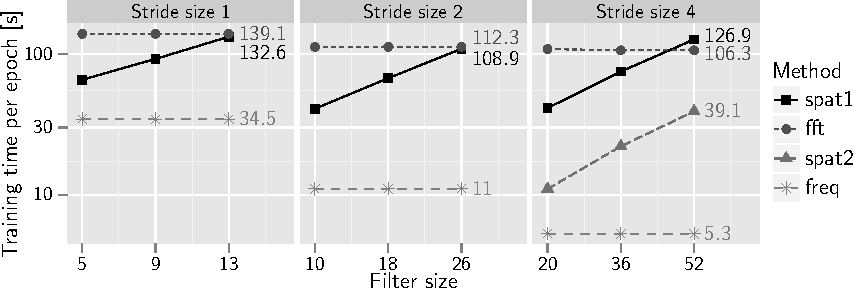
\includegraphics{figures/NECO-03-14-2099-Figure-2}
%\input{r_figures/runtime_imgnet_c3_bw}
}

\subfloat[Running times of training a second layer sconvRBM with
16, 32, and 64 channels (stride size 1).] {
\label{fig:run_imgnet_l2}
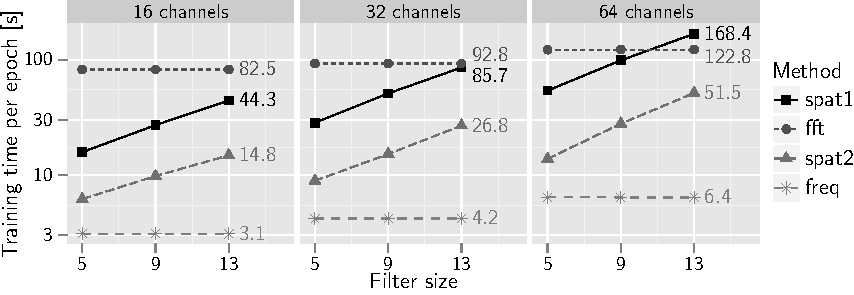
\includegraphics{figures/NECO-03-14-2099-Figure-3}
%\input{r_figures/runtime_imgnet_c16-64_bw}
}

\label{fig:run_imgnet}
\caption{Comparison of running times for training a (a) first and
(b) second layer sconvRBM on 2D images using our frequency domain method (freq) and three
alternative methods using different convolution implementations: single image
convolutions (spat1), batched convolutions (spat2), and convolution by using
FFTs (fft). Due to internal limitations of the implementation of batched
convolutions, a comparison with spat2 could not be performed for images with a
resolution of \num{512x512} when using a stride size smaller than four.}
\end{figure}

Figure~\ref{fig:run_imgnet_l2} shows a similar comparison for training the
second convRBM layer for a stride size of 1 and varying filter sizes and numbers
of channels. In contrast to training the first layer, training times mostly
depend on the calculation of convolutions, where the impact of calculating
convolutions on the total running time increases with an increasing number of
channels. Training in the frequency domain is between 5 to 26 times faster than
training in the spatial domain using single-image convolutions, and 2
to 8 times faster than using batched convolutions. For all channel sizes,
batched training is about 3 to 4 times faster than non-batched training and
calculating convolutions using FFTs is much slower than batched training and
training in the frequency domain. To summarize, training of 2D images in the
frequency domain is much faster than training in the spatial domain even for
small filter sizes.
Using the largest filter kernels in both layers, the proposed method is shown to
yield a speedup of 7 to 8 times compared to state-of-the-art GPU
implementations.

\subsection{Running Time Analysis on 3D Volumes (OASIS)}

Figure~\ref{fig:run_oasis} shows the comparison of running times for training a
first  and second layer sconvRBM on 3D volumes for varying filter sizes, stride
sizes, and varying numbers of channels. In contrast to training on 2D images,
the computational costs of calculating 3D convolutions break even with
calculating FFTs for small filter sizes, because the number of multiplications
and additions per convolution increases cubically, instead of quadratically,
with the filter kernel size. As a result, simply training by convolutions in the
frequency domain is faster than in the spatial domain. However, our proposed
training algorithm still outperforms both other methods, even at the smallest
filter size. For filter sizes of 5 and larger, our frequency domain
implementation is between 3.5 to 200 times faster than our spatial domain
implementation using single-image convolutions and 2.7 to 17 times faster than
calculating convolutions by FFTs. Similar to the results on 2D images, training
times of the first layer using a stride of 1 depend strongly on the time
required to calculate the expectation of the hidden units and to sample the
hidden units. Hence, performance improvements of our frequency domain method are
more pronounced for larger strides and numbers of channels, where the impact of
calculating convolutions on the total training time is also larger. This makes
the proposed method particularly suitable for training sconvRBMs on
high-resolution 3D volumes.

\begin{figure}[t!]
\subfloat[Running times of training a first layer sconvRBM with stride sizes of 1, 2, and 4.] {
\label{fig:run_oasis_l1}
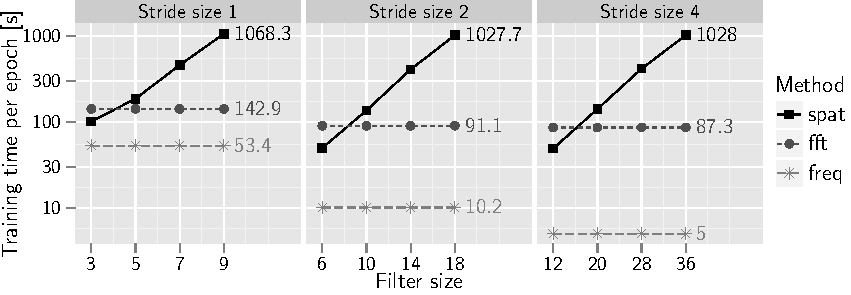
\includegraphics{figures/NECO-03-14-2099-Figure-4}
%\input{r_figures/runtime_oasis_c1_bw}
}

\subfloat[Running times of training a second layer sconvRBM with 8, 16, and 32
channels (stride size 1).] {
\label{fig:run_oasis_l2}
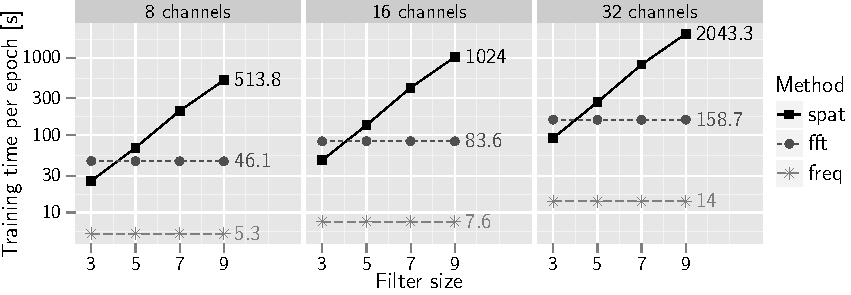
\includegraphics{figures/NECO-03-14-2099-Figure-5}
%\input{r_figures/runtime_oasis_c8-32_bw}
}
\caption{Comparison of running times for training a (a) first and (b) second
layer sconvRBM on 3D volumes using a single 3D image convolution implementation
(spat), an implementation that calculates convolutions by using FFTs (fft), and
our proposed implementation in the frequency domain (freq).}
\label{fig:run_oasis}
\end{figure}


\chapter{Modeling the Variability of Brain MRIs}

\section{Variability and Manifold Learning}

% Start with section on manifold learning of AD and MS
% populations. Including a summary of those methods and the whole literature
% review of what has been done. This includes manifold learning, population
% studies, disease classification and the likes without deep learning.

The need for manifold learning often arises when very high-dimensional data
needs to be analyzed but the intrinsic dimensionality of the data is much lower.
This situations occurs, for example, when trying to visualize variability and
common patterns in a given group of magnetic resonance images (MRIs) of the
brain. Each image can be regarded as a point in a high-dimensional image space
(called the ambient space), with $n_x \times n_y \times n_z$ coordinates, where
$n_x, n_y, n_z$ are the dimensions of each image. On the other hand, each image
could also be identified by a smaller set of parameters that describe shape
variations and patterns that are common for a particular group of images. These
parameters span a new space called the manifold space. The task of manifold
learning is to discover the low-dimensional space and its parameters which can
then be used to model the anatomical variability within a population.

Various methods for manifold learning have been proposed (e.g., locally linear
embedding (LLE) \citep{saul2003}, Laplacian eigenmaps (LEM) \citep{belkin2002},
Isomaps \citep{tenenbaum2000}), with Isomaps and LEM being the most popular for
medical image analysis. Both methods require a prebuild proximity graph. In
order to build the proximity graph, it is assumed that the manifold space is
locally linear, which means that distances between neighboring points in
manifold space can be approximated by their distances in ambient space. Gerber
et. al. have shown that the choice of a suitable distance measure is crucial
for manifold learning using Isomaps and that the warping distance between brain images
improves the learning performance over previously used Euclidean distances in
the image space \citep{gerber2010}.

% Talk about applications

Manifolds have been used to regularize the segmentation of brain
ventricles~\citep{etyngier2007}, and to constrain the deformable registration of
brain images to have biologically plausible parameters \citep{hamm2010}. Gerber
et al. used Isomaps to predict clinical parameters of Alzheimers's (AD) patients
\citep{gerber2010}, and Wolz et al. used Laplacian eigenmaps to perform
biomarker discovery \citep{wolz2011}, also of AD patients, and atlas propagation
for the segmentation of the hippocampus \citep{wolz2010}.

% TODO: Take the MS motivation out into a separate MS part.

Other application in the area of MS. Multiple sclerosis (MS) is an inflammatory
and degenerative disease of the central nervous system with pathology that can
be observed in vivo by magnetic resonance imaging (MRI). MS is characterized by
the formation of lesions, primarily visible in white matter on conventional MRI,
and the death of nervous tissue leading to global and regional atrophy. A number
of imaging biomarkers, such as lesion volume and whole brain volume, have
established their importance for the study of MS. However, MS is a complex
disease whose pathological variability extends well beyond what can be captured
by global and local volumetric measures. Methods based on statistics of
diffeomorphisms have been used to discover patterns of regional atrophy
\cite{Ceccarelli2012}, but they are not designed to directly model morphological
variability. It would be highly desirable to have a method that can
automatically discover potentially important patterns of variability in brain
morphology and lesion distribution, which would advance our understanding of the
complex pathology of MS. In addition, the joint modeling of brain morphology and
lesion distribution would further our knowledge of how these two key
pathological features interact. However, this type of modeling is very
challenging due to the high dimensionality of the data. In recent years, there
has been an increased interest in biomarker discovery using manifold learning to
form high-level representations of medical images
\cite{Wolz2010b,AljabarRueckert2011,Wolz2012}. Manifold learning is motivated by
the assumption that the space of brain images can be modeled to some
approximation by a low-dimensional manifold. Various methods for manifold
learning have been proposed (e.g., locally linear embedding (LLE), Laplacian
eigenmaps (LEM), Isomaps) \cite{Cayton2005}, with Isomaps and LEM being the most
popular for medical image analysis. Most such methods require a prebuilt
proximity graph based on a selected distance measure, the choice of which can be
crucial for manifold learning \cite{Gerber2010}. Aljabar et al. proposed a
method \cite{AljabarRueckert2011} for the joint modeling of multiple image
features of neonatal brains. First, separate manifolds based on features from
geometric surface models, non-rigid deformations, and image intensities are
learned, then a second dimensionality reduction step is used to combine the
individual manifold parameters.

\section{Manifold of AD Patients}

% Motivation and short overview of the method and why use this one and not
% alternatives. What data was used? Applied to RAW MRI images without much
% preprocessing.

In this paper, we propose a novel approach for learning the manifold of brain
images that uses a deep belief network (DBN) \cite{Hinton2006b} to discover
patterns of similarity in groups of images. In contrast to previous
brain manifold learning algorithms, DBNs do not assume the manifold
space to be locally linear and do not require a previously defined similarity
measure or the construction of a proximity graph.
\begin{itemize}
\item DBNs mostly limited to 2D images, still the case?
\item Our fast training method allows DBNs to be used for manifold learning of
3D medical images
\end{itemize}

Contribution is the demonstration that DBNs can learn a low-dimensional manifold
of brain volumes that detects modes of variation that correlate to demographic
and disease parameters.

\subsection{Method}

% Explain the method in more detail. Also what tools where used for the
% experiments and stuff. How was the DBN designed and why.

% TODO: Less math an more model. Maybe draw the entire model in a figure or at
% least have a table with the parameters. Emphasise use of a strided
% convolutional RBM for dimensionality reduction

% TODO: Fuse this with the rest of the text. Look at MICCAI 2014 to know how.

We have evaluated the proposed method on a subset of the ADNI dataset
\cite{Petersen2010}, containing 300 T1-weighted MRIs of Alzheimer's disease (AD)
and normal subjects. The images were provided skull-stripped and bias field
corrected. We resampled all images to a resolution of \num{128x128x128} voxels
and a voxel size of \SI{2.0x2.0x2.0}{\milli\meter}. We then normalized their
intensities to a common range, and rigidly registered them to a group-wise mean
image prior to training and testing. We did not perform non-rigid registration
for spatial normalization in order to evaluate the capabilities of the method
without the added confound of complex registration parameters. The dataset was
divided into a training set and a test set such that each set contains 75 AD and
75 normal subjects. To learn the manifold of brain MRIs, we used a DBN with
three convRBM layers and two RBM layers. After three convRBMs, the dimension of
each image is reduced to \num{8x8x8} and small enough for RBMs. The training of
the DBN took approximately 43 hours on two GeForce GTX 560 Ti graphics cards.

Our proposed method performs manifold learning by reducing the dimensionality of
the input images using a DBN, a deep generative model that is composed of
multiple restricted Boltzmann machines (RBMs)~\cite{Hinton2006b} as illustrated
by the simplified example in Fig.~\ref{fig:rbmscheme}.
% TODO: No simplified model. The real model is needed.
An RBM is a Markov random
field with trainable weights whose nodes are divided into a visible layer
$\vect{v}$ representing the inputs of the model and a hidden layer $\vect{h}$
representing extracted features from the inputs. The first RBM receives the
intensity values of a group of images as input and reduces the dimensionality of
each image by discovering patterns of similarity that are common within groups
of images. Subsequent RBMs receive the hidden unit activations of the previous
RBM as input, thus learning successively more complex and abstract patterns from
a training set. The number of trainable weights increases significantly with the
resolution of the training images. In order to scale the model to
high-resolution images, the first several layers of our DBN are convolutional
RBMs (convRBMs), a type of RBM that uses weight sharing to reduce the number of
trainable weights, albeit at the cost of using the much more computationally
expensive convolutions instead of multiplications. In the remainder of this
section, we will briefly review the training of convRBMs, followed by a
description of our novel training algorithm that performs parameter learning in
frequency domain. For comprehensive introductions to RBMs and convRBMs, the
reader is referred to \cite{Hinton2006b} and \cite{Lee2011}, respectively.

Our algorithm for the dimensionality reduction of an input image using a
convRBM is illustrated in Fig.~\ref{fig:convrbm}. In contrast to previous work
that uses max pooling to reduce the dimensionality \cite{Lee2011}, all steps
involved in our method are invertible, which allows the reconstruction of
images from their manifold coordinates. In the first step, the pixels of an
input image are reorganized into multiple images of lower resolution in order to
reduce the dimensionality of a single image. The number of images in the image
vector is then reduced with the following steps.
To apply the model to real-valued data like the intensities of some medical
images, the visible units are modeled as Gaussian units. When the visible units have
been mean centered and standardized to unit variance, the expectation of the
visible units is given by
\begin{equation} 
\E[v_i \given \vect{h}] = \textstyle\sum_j w_{ij}*h_j + b_i
\label{eq:convvis}
\end{equation}
where $v_i, h_j, b_i \in \R^{N \times N \times N}$, $b_i$ are bias terms, $N$ is
the image size, $w_{ij} \in \R^{N_w \times N_w \times N_w}$ are the weights,
$N_w$ is the size of a weight kernel, and $*$ denotes circular convolution.
A binary hidden unit can only encode two states. In order to increase the
expressive power of the hidden units, we use noisy rectified
linear units as the hidden units,
which has shown to improve the learning performance~\cite{Nair2010} of RBMs.
The
hidden units can be sampled with
\begin{equation} 
h_j \sim \max(0, \mu_j + \Norm(0, \sigm(\mu_j)))
\label{eq:convhid}
\end{equation} 
where $\mu_j = \textstyle\sum_i\tilde{w}_{ij}*v_i +c_j$, $c_j \in \R^{N \times
N \times N}$, $\tilde{w}$ denotes a flipped version of $w$ in all three
dimensions, $\Norm(0, \sigma^2)$ denotes Gaussian noise, and $\sigm(x)$ is the
sigmoid function defined as $\sigm(x) = (1+ \exp(-x))^{-1}, x \in \R$. The
weights and bias terms of a convRBM can be learned using contrastive
divergence (CD) \cite{Hinton2006b}. During each iteration of the algorithm, the
gradient of the parameters is estimated and a gradient step with a fixed
learning rate is performed. The gradient of the weights can be approximated by:
\begin{equation}
\Delta w_{ij} = v_i*\tilde{h}_j - v_i'*\tilde{h}_j'
\label{eq:convgra}
\end{equation}
where $h_j$ and $h_j'$ are samples drawn from $p(h_j \given \vect{v})$ and
$p(h_j \given \vect{v}')$ using \eqref{eq:convhid} and $v_i' = \E[v_i \given
\vect{h}]$.

\subsection{Evaluation}

The geometric fit of the learned manifold model was evaluated in terms of the
generalizability to new images and the specificity to images from the training
set. The generalizability was measured as the average root mean squared error
(RMSE) between an image and its reconstruction, normalized by the intensity
range of the input image. The specificity was measured by calculating the
average RMSE between images randomly generated from the manifold model and the
most similar images from the training set. Figure~\ref{fig:genspe}(a) shows a
comparison of the reconstruction errors between the training and test sets, and
the specificity at different layers of the DBN. The similarity of the
reconstruction errors between the training and test images indicates that no
overfitting is occurring. The average reconstruction error at the last layer is
below \SI{6}{\percent}. Even though the very small reconstruction error is
partially due to head MRIs having a large amount of homogeneous background, it
demonstrates the ability of the learned manifold to capture most of the visual
information with only two manifold parameters. The opposite slopes of the
reconstruction errors and error of generated images indicates a trade-off
between generalizability and specificity in the earlier phases of training. The
low errors at the end of training (Layer 5) indicates that the method is able to
be both specific and generalizable.

\begin{figure}[tb]
\centering
\subfloat[Generalizability vs. specificity]{
  % Created by tikzDevice version 0.6.2-92-0ad2792 on 2013-06-06 10:46:52
% !TEX encoding = UTF-8 Unicode
\begin{tikzpicture}[x=1pt,y=1pt]
\tikzstyle{clip}=[]
\definecolor[named]{fillColor}{rgb}{1.00,1.00,1.00}
\path[use as bounding box,fill=fillColor,fill opacity=0.00] (0,0) rectangle (169.83,130.09);
\begin{scope}
\path[clip] ( 33.55, 24.84) rectangle (169.83,106.43);
\definecolor[named]{fillColor}{rgb}{0.90,0.90,0.90}

\path[fill=fillColor] ( 33.55, 24.84) rectangle (169.83,106.43);
\definecolor[named]{drawColor}{rgb}{0.95,0.95,0.95}

\path[draw=drawColor,line width= 0.3pt,line join=round] ( 33.55, 35.47) --
	(169.83, 35.47);

\path[draw=drawColor,line width= 0.3pt,line join=round] ( 33.55, 51.46) --
	(169.83, 51.46);

\path[draw=drawColor,line width= 0.3pt,line join=round] ( 33.55, 67.46) --
	(169.83, 67.46);

\path[draw=drawColor,line width= 0.3pt,line join=round] ( 33.55, 83.45) --
	(169.83, 83.45);

\path[draw=drawColor,line width= 0.3pt,line join=round] ( 33.55, 99.44) --
	(169.83, 99.44);

\path[draw=drawColor,line width= 0.3pt,line join=round] ( 55.23, 24.84) --
	( 55.23,106.43);

\path[draw=drawColor,line width= 0.3pt,line join=round] ( 86.21, 24.84) --
	( 86.21,106.43);

\path[draw=drawColor,line width= 0.3pt,line join=round] (117.18, 24.84) --
	(117.18,106.43);

\path[draw=drawColor,line width= 0.3pt,line join=round] (148.15, 24.84) --
	(148.15,106.43);
\definecolor[named]{drawColor}{rgb}{1.00,1.00,1.00}

\path[draw=drawColor,line width= 0.6pt,line join=round] ( 33.55, 27.47) --
	(169.83, 27.47);

\path[draw=drawColor,line width= 0.6pt,line join=round] ( 33.55, 43.47) --
	(169.83, 43.47);

\path[draw=drawColor,line width= 0.6pt,line join=round] ( 33.55, 59.46) --
	(169.83, 59.46);

\path[draw=drawColor,line width= 0.6pt,line join=round] ( 33.55, 75.45) --
	(169.83, 75.45);

\path[draw=drawColor,line width= 0.6pt,line join=round] ( 33.55, 91.45) --
	(169.83, 91.45);

\path[draw=drawColor,line width= 0.6pt,line join=round] ( 39.75, 24.84) --
	( 39.75,106.43);

\path[draw=drawColor,line width= 0.6pt,line join=round] ( 70.72, 24.84) --
	( 70.72,106.43);

\path[draw=drawColor,line width= 0.6pt,line join=round] (101.69, 24.84) --
	(101.69,106.43);

\path[draw=drawColor,line width= 0.6pt,line join=round] (132.67, 24.84) --
	(132.67,106.43);

\path[draw=drawColor,line width= 0.6pt,line join=round] (163.64, 24.84) --
	(163.64,106.43);
\definecolor[named]{drawColor}{rgb}{0.38,0.61,1.00}

\path[draw=drawColor,line width= 0.6pt,line join=round] ( 39.75, 28.55) --
	( 70.72, 35.28) --
	(101.69, 39.23) --
	(132.67, 40.14) --
	(163.64, 40.37);
\definecolor[named]{drawColor}{rgb}{0.00,0.73,0.22}

\path[draw=drawColor,line width= 0.6pt,line join=round] ( 39.75, 29.66) --
	( 70.72, 37.10) --
	(101.69, 41.49) --
	(132.67, 41.93) --
	(163.64, 42.24);
\definecolor[named]{drawColor}{rgb}{0.97,0.46,0.43}

\path[draw=drawColor,line width= 0.6pt,line join=round] ( 39.75,102.72) --
	( 70.72, 94.58) --
	(101.69, 78.65) --
	(132.67, 39.60) --
	(163.64, 35.60);
\end{scope}
\begin{scope}
\path[clip] (  0.00,  0.00) rectangle (169.83,130.09);
\definecolor[named]{drawColor}{rgb}{0.00,0.00,0.00}

\node[text=drawColor,anchor=base east,inner sep=0pt, outer sep=0pt, scale=  0.80] at ( 26.44, 24.72) {0.04};

\node[text=drawColor,anchor=base east,inner sep=0pt, outer sep=0pt, scale=  0.80] at ( 26.44, 40.71) {0.06};

\node[text=drawColor,anchor=base east,inner sep=0pt, outer sep=0pt, scale=  0.80] at ( 26.44, 56.71) {0.08};

\node[text=drawColor,anchor=base east,inner sep=0pt, outer sep=0pt, scale=  0.80] at ( 26.44, 72.70) {0.10};

\node[text=drawColor,anchor=base east,inner sep=0pt, outer sep=0pt, scale=  0.80] at ( 26.44, 88.69) {0.12};
\end{scope}
\begin{scope}
\path[clip] (  0.00,  0.00) rectangle (169.83,130.09);
\definecolor[named]{drawColor}{rgb}{0.50,0.50,0.50}

\path[draw=drawColor,line width= 0.6pt,line join=round] ( 29.29, 27.47) --
	( 33.55, 27.47);

\path[draw=drawColor,line width= 0.6pt,line join=round] ( 29.29, 43.47) --
	( 33.55, 43.47);

\path[draw=drawColor,line width= 0.6pt,line join=round] ( 29.29, 59.46) --
	( 33.55, 59.46);

\path[draw=drawColor,line width= 0.6pt,line join=round] ( 29.29, 75.45) --
	( 33.55, 75.45);

\path[draw=drawColor,line width= 0.6pt,line join=round] ( 29.29, 91.45) --
	( 33.55, 91.45);
\end{scope}
\begin{scope}
\path[clip] (  0.00,  0.00) rectangle (169.83,130.09);
\definecolor[named]{drawColor}{rgb}{0.50,0.50,0.50}

\path[draw=drawColor,line width= 0.6pt,line join=round] ( 39.75, 20.58) --
	( 39.75, 24.84);

\path[draw=drawColor,line width= 0.6pt,line join=round] ( 70.72, 20.58) --
	( 70.72, 24.84);

\path[draw=drawColor,line width= 0.6pt,line join=round] (101.69, 20.58) --
	(101.69, 24.84);

\path[draw=drawColor,line width= 0.6pt,line join=round] (132.67, 20.58) --
	(132.67, 24.84);

\path[draw=drawColor,line width= 0.6pt,line join=round] (163.64, 20.58) --
	(163.64, 24.84);
\end{scope}
\begin{scope}
\path[clip] (  0.00,  0.00) rectangle (169.83,130.09);
\definecolor[named]{drawColor}{rgb}{0.00,0.00,0.00}

\node[text=drawColor,anchor=base,inner sep=0pt, outer sep=0pt, scale=  0.80] at ( 39.75, 12.22) {1};

\node[text=drawColor,anchor=base,inner sep=0pt, outer sep=0pt, scale=  0.80] at ( 70.72, 12.22) {2};

\node[text=drawColor,anchor=base,inner sep=0pt, outer sep=0pt, scale=  0.80] at (101.69, 12.22) {3};

\node[text=drawColor,anchor=base,inner sep=0pt, outer sep=0pt, scale=  0.80] at (132.67, 12.22) {4};

\node[text=drawColor,anchor=base,inner sep=0pt, outer sep=0pt, scale=  0.80] at (163.64, 12.22) {5};
\end{scope}
\begin{scope}
\path[clip] (  0.00,  0.00) rectangle (169.83,130.09);
\definecolor[named]{drawColor}{rgb}{0.00,0.00,0.00}

\node[text=drawColor,anchor=base,inner sep=0pt, outer sep=0pt, scale=  0.90] at (101.69,  3.01) {Layer};
\end{scope}
\begin{scope}
\path[clip] (  0.00,  0.00) rectangle (169.83,130.09);
\definecolor[named]{drawColor}{rgb}{0.00,0.00,0.00}

\node[text=drawColor,rotate= 90.00,anchor=base,inner sep=0pt, outer sep=0pt, scale=  0.90] at (  9.21, 65.64) {RMSE};
\end{scope}
\begin{scope}
\path[clip] (  0.00,  0.00) rectangle (169.83,130.09);
\definecolor[named]{fillColor}{rgb}{1.00,1.00,1.00}

\path[fill=fillColor] ( -4.49,106.76) rectangle (207.88,129.75);
\end{scope}
\begin{scope}
\path[clip] (  0.00,  0.00) rectangle (169.83,130.09);
\definecolor[named]{drawColor}{rgb}{1.00,1.00,1.00}
\definecolor[named]{fillColor}{rgb}{0.95,0.95,0.95}

\path[draw=drawColor,line width= 0.6pt,line join=round,line cap=round,fill=fillColor] (  3.39,111.03) rectangle ( 17.85,125.49);
\end{scope}
\begin{scope}
\path[clip] (  0.00,  0.00) rectangle (169.83,130.09);
\definecolor[named]{drawColor}{rgb}{0.97,0.46,0.43}

\path[draw=drawColor,line width= 0.6pt,line join=round] (  4.84,118.26) -- ( 16.40,118.26);
\end{scope}
\begin{scope}
\path[clip] (  0.00,  0.00) rectangle (169.83,130.09);
\definecolor[named]{drawColor}{rgb}{0.97,0.46,0.43}

\path[draw=drawColor,line width= 0.6pt,line join=round] (  4.84,118.26) -- ( 16.40,118.26);
\end{scope}
\begin{scope}
\path[clip] (  0.00,  0.00) rectangle (169.83,130.09);
\definecolor[named]{drawColor}{rgb}{0.97,0.46,0.43}

\path[draw=drawColor,line width= 0.6pt,line join=round] (  4.84,118.26) -- ( 16.40,118.26);
\end{scope}
\begin{scope}
\path[clip] (  0.00,  0.00) rectangle (169.83,130.09);
\definecolor[named]{drawColor}{rgb}{1.00,1.00,1.00}
\definecolor[named]{fillColor}{rgb}{0.95,0.95,0.95}

\path[draw=drawColor,line width= 0.6pt,line join=round,line cap=round,fill=fillColor] ( 80.31,111.03) rectangle ( 94.76,125.49);
\end{scope}
\begin{scope}
\path[clip] (  0.00,  0.00) rectangle (169.83,130.09);
\definecolor[named]{drawColor}{rgb}{0.00,0.73,0.22}

\path[draw=drawColor,line width= 0.6pt,line join=round] ( 81.76,118.26) -- ( 93.32,118.26);
\end{scope}
\begin{scope}
\path[clip] (  0.00,  0.00) rectangle (169.83,130.09);
\definecolor[named]{drawColor}{rgb}{0.00,0.73,0.22}

\path[draw=drawColor,line width= 0.6pt,line join=round] ( 81.76,118.26) -- ( 93.32,118.26);
\end{scope}
\begin{scope}
\path[clip] (  0.00,  0.00) rectangle (169.83,130.09);
\definecolor[named]{drawColor}{rgb}{0.00,0.73,0.22}

\path[draw=drawColor,line width= 0.6pt,line join=round] ( 81.76,118.26) -- ( 93.32,118.26);
\end{scope}
\begin{scope}
\path[clip] (  0.00,  0.00) rectangle (169.83,130.09);
\definecolor[named]{drawColor}{rgb}{1.00,1.00,1.00}
\definecolor[named]{fillColor}{rgb}{0.95,0.95,0.95}

\path[draw=drawColor,line width= 0.6pt,line join=round,line cap=round,fill=fillColor] (135.08,111.03) rectangle (149.54,125.49);
\end{scope}
\begin{scope}
\path[clip] (  0.00,  0.00) rectangle (169.83,130.09);
\definecolor[named]{drawColor}{rgb}{0.38,0.61,1.00}

\path[draw=drawColor,line width= 0.6pt,line join=round] (136.53,118.26) -- (148.09,118.26);
\end{scope}
\begin{scope}
\path[clip] (  0.00,  0.00) rectangle (169.83,130.09);
\definecolor[named]{drawColor}{rgb}{0.38,0.61,1.00}

\path[draw=drawColor,line width= 0.6pt,line join=round] (136.53,118.26) -- (148.09,118.26);
\end{scope}
\begin{scope}
\path[clip] (  0.00,  0.00) rectangle (169.83,130.09);
\definecolor[named]{drawColor}{rgb}{0.38,0.61,1.00}

\path[draw=drawColor,line width= 0.6pt,line join=round] (136.53,118.26) -- (148.09,118.26);
\end{scope}
\begin{scope}
\path[clip] (  0.00,  0.00) rectangle (169.83,130.09);
\definecolor[named]{drawColor}{rgb}{0.00,0.00,0.00}

\node[text=drawColor,anchor=base west,inner sep=0pt, outer sep=0pt, scale=  0.85] at ( 19.65,115.33) {Specificity error};
\end{scope}
\begin{scope}
\path[clip] (  0.00,  0.00) rectangle (169.83,130.09);
\definecolor[named]{drawColor}{rgb}{0.00,0.00,0.00}

\node[text=drawColor,anchor=base west,inner sep=0pt, outer sep=0pt, scale=  0.85] at ( 96.57,115.33) {Test error};
\end{scope}
\begin{scope}
\path[clip] (  0.00,  0.00) rectangle (169.83,130.09);
\definecolor[named]{drawColor}{rgb}{0.00,0.00,0.00}

\node[text=drawColor,anchor=base west,inner sep=0pt, outer sep=0pt, scale=  0.85] at (151.34,115.33) {Training error};
\end{scope}
\end{tikzpicture}

}\qquad \quad\quad 
\subfloat[Generated images]{
  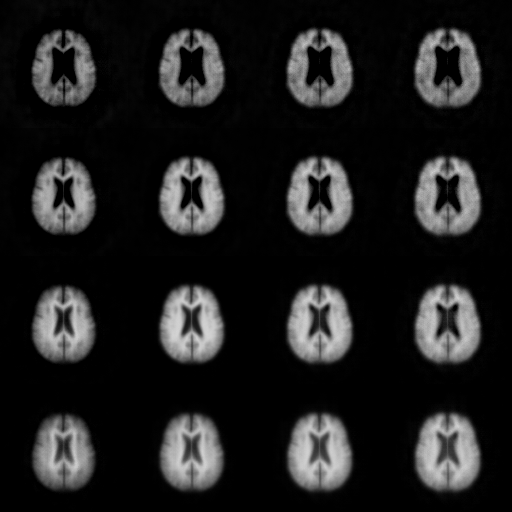
\includegraphics[width=0.3\textwidth, trim=0 -4em 0 0]
  {figures/MICCAI2013_sampled2d}
} 

\caption{(a) The similarity of the reconstruction errors between the training
and test images indicates that no overfitting occurs. The opposite slopes of the
reconstruction errors and error of generated images (specificity error)
indicates a trade-off between generalizability vs. specificity in the earlier
phases of training, but the low errors at Layer 5 indicate that the method is
both generalizable and specific.
(b) Axial slices from generated volumes from the manifold. An increase of the
first and second manifold dimension visually correlates with an increase in
brain and ventricle size, respectively.}
\label{fig:genspe}
\end{figure}

Figure~\ref{fig:genspe}(b) shows axial slices of 16 volumes sampled at the
grid points of a 2D regular grid in manifold space. Volumes sampled along the
first manifold dimension (from left to right) appear to increase in brain size,
and the images sampled along the second manifold dimension (from bottom to top)
appear to increase in ventricle size. Figure~\ref{fig:scatter} shows an axial slice of
each image of the training set plotted against its manifold coordinates.
Consistent with images sampled from the manifold, an increase in ventricle size,
which is indicative of brain atrophy (a hallmark of AD), visually correlates
with an increase of the second manifold coordinate.
The AD/normal status is indicated by the frame color of each image. The vertical
separation between AD and normals suggests that the second manifold coordinate is
potentially of practical use in differentiating between AD and normal.

\begin{figure}[tb] \centering
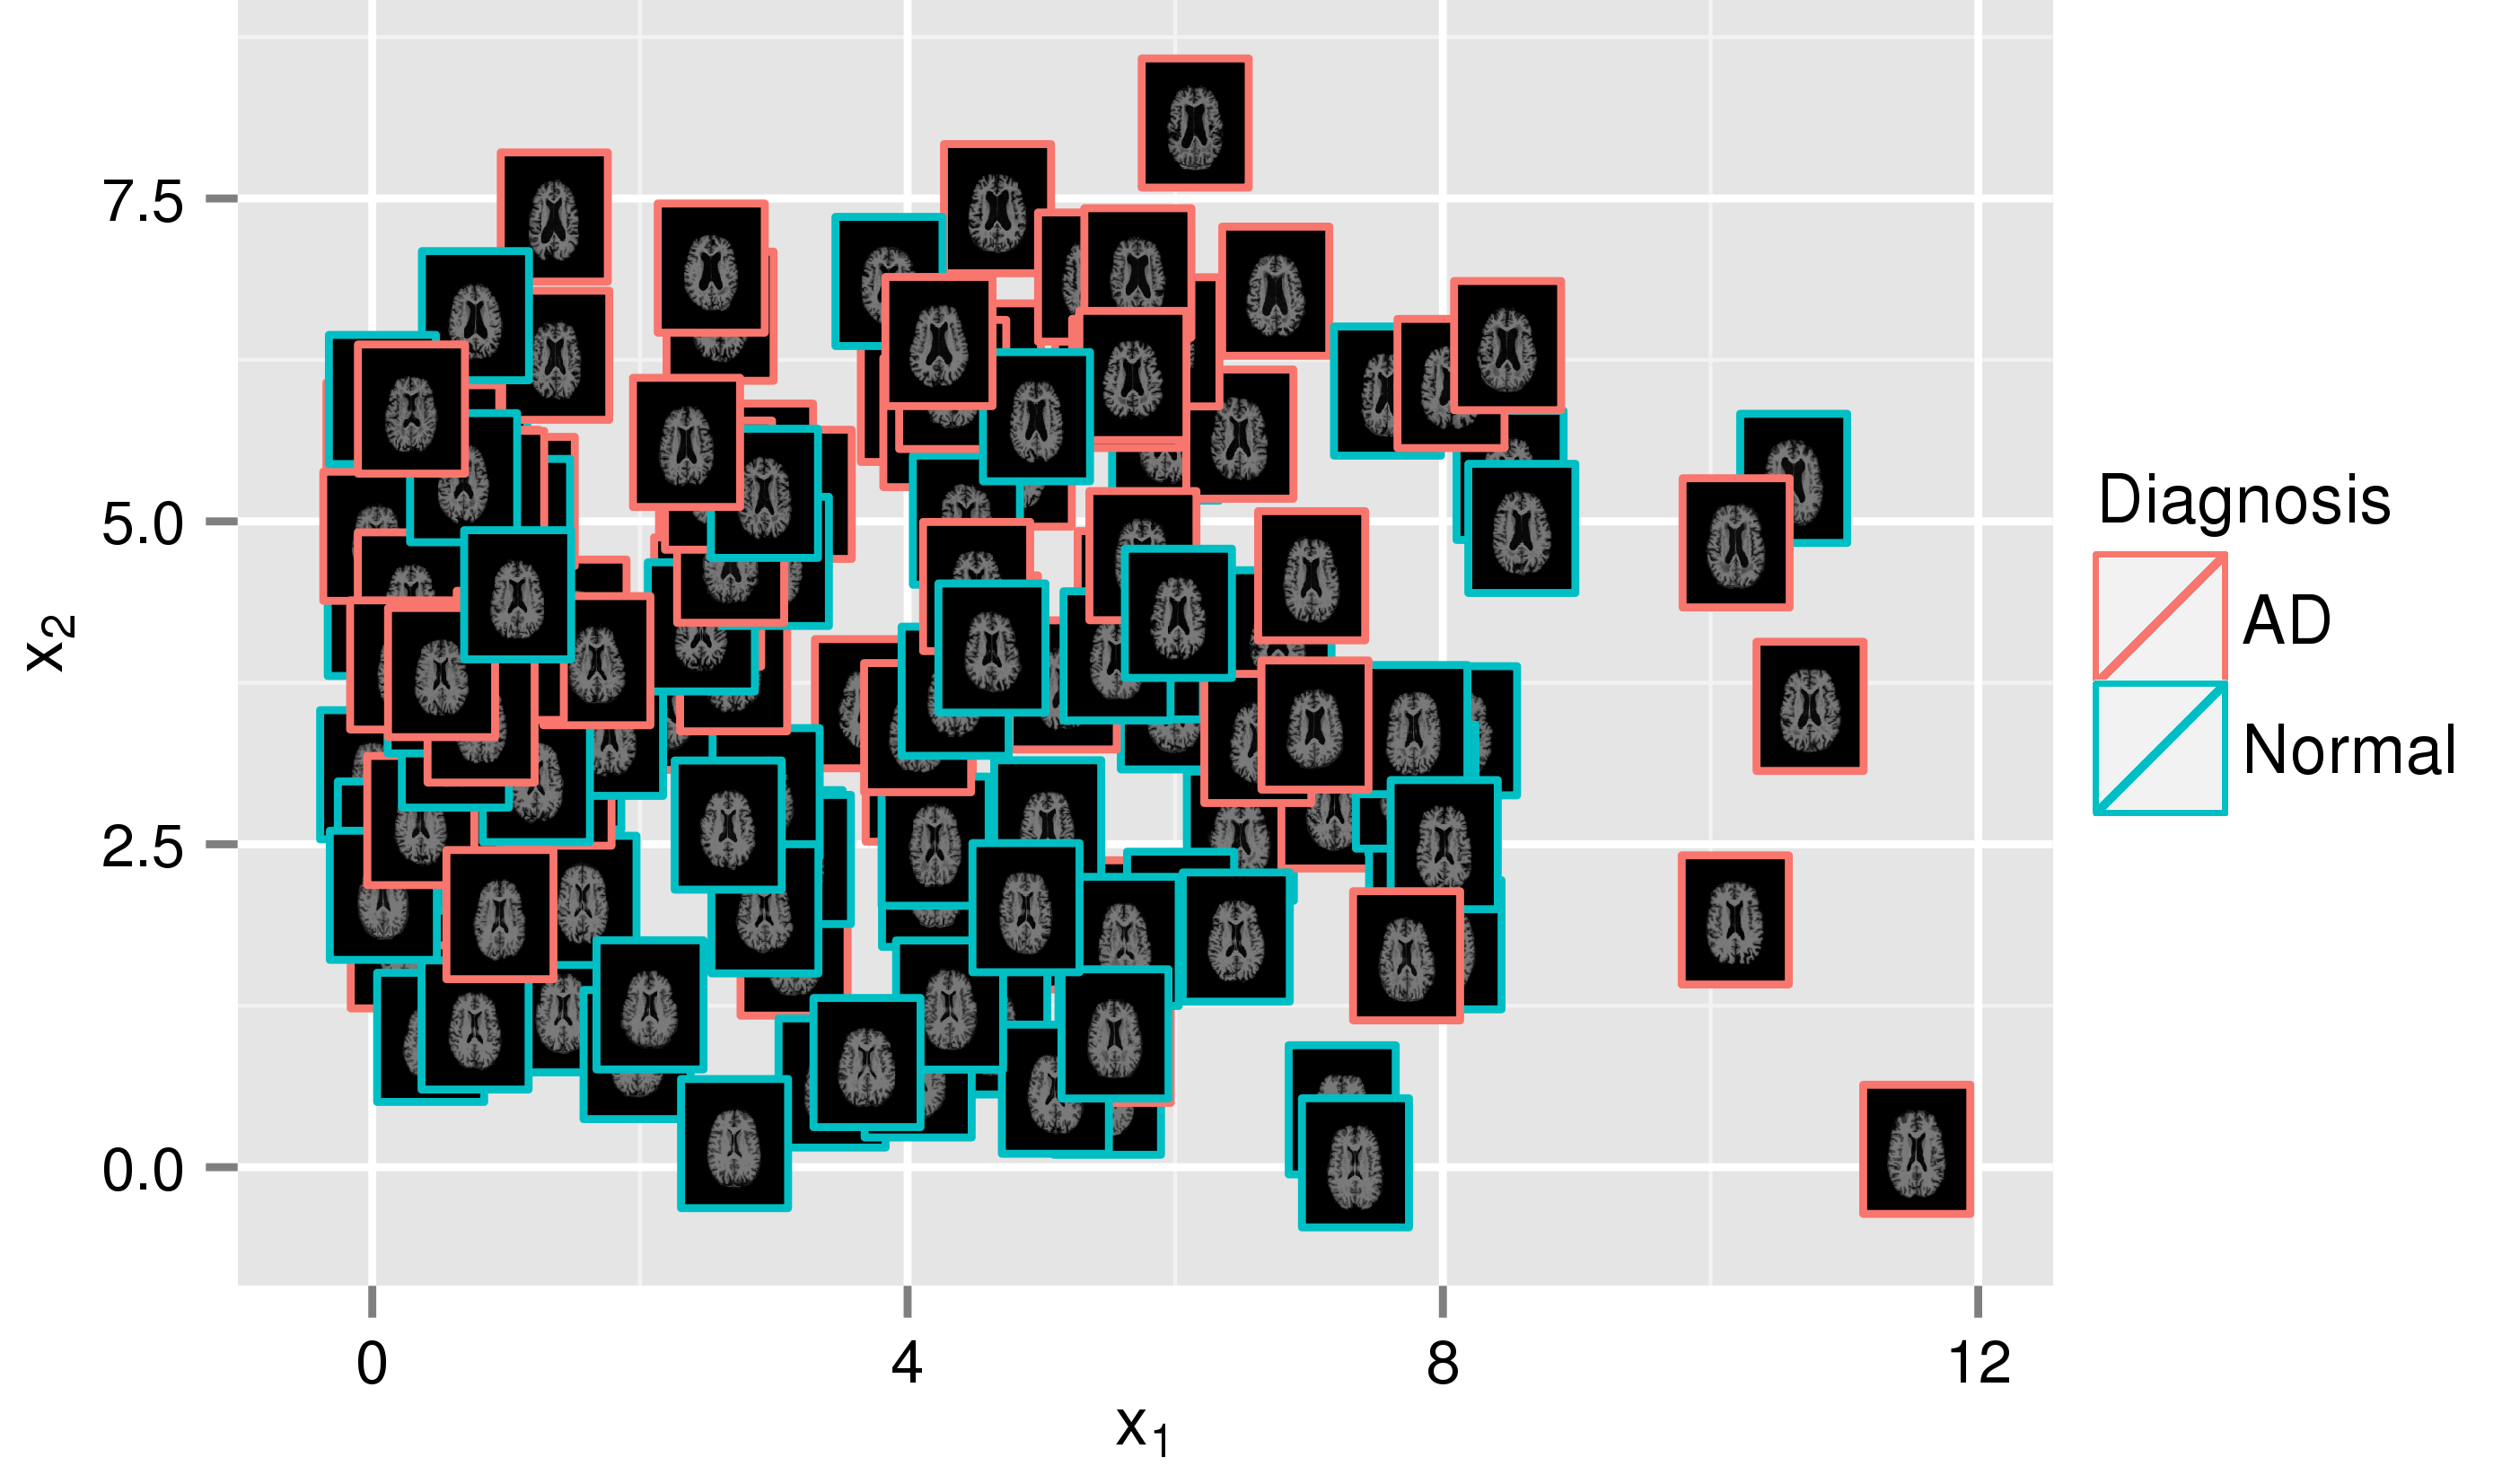
\includegraphics[width=0.75\textwidth]{figures/MICCAI2013_scatter3}
\caption{Axial slices of volumes from the training set plotted against their
manifold coordinates. The brains with larger ventricles, indicative of atrophy,
are mostly at the top, which is also where most of the AD patients are.}
\label{fig:scatter}
\end{figure}

To evaluate the potential of the manifold coordinates to reveal or predict
clinically relevant information, we have calculated the Pearson correlation $r$
of demographic parameters (age, gender) and disease parameters (mini-mental
state examination (MMSE) score, AD/normal status) with the manifold coordinates
($x_1$ and $x_2$). The results of the correlation tests are summarized in
Table~\ref{tab:corr}. Age, MMSE and AD/normal status show highly significant
correlations with $x_2$ ($p$-values between \num{9.85e-9} and \num{3.53e-7}),
which makes intuitive sense because $x_2$ visually correlates with ventricle
size. The first manifold coordinate correlates strongest with gender
($p\text{-value} = \num{8.24e-9}$), which also makes sense in terms of the
general difference in size between male and female. The strength and
significance of the correlations demonstrate the potential of deep learning of
brain images for classification and prediction of disease status.

\begin{table}[tb]
\small
\centering
\caption{Pearson correlation $r$ of demographic and clinical parameters with
manifold coordinates ($x_1$, $x_2$). The stronger correlation in each column is
highlighted in bold.}
\sisetup{
  round-mode = places,
  round-precision = 2,
  exponent-product = \cdot,
  detect-weight=true,detect-inline-weight=math,
  tight-spacing = true
}%

\begin{tabular}{l*{4}{@{\hspace{15pt}}cc}}
\toprule
& \multicolumn{2}{c}{Age} & \multicolumn{2}{c}{Gender} &
\multicolumn{2}{c}{MMSE} & \multicolumn{2}{c}{AD/Normal Status} \\
& $r$ & $p$-value & $r$ & $p$-value & $r$ & $p$-value
& $r$ & $p$-value \\
\midrule
% V1
$x_1$ &
\num{-0.1734} & \num{0.03378} &
\textbf{\num{0.4490381}} & \textbf{\num{8.239e-09}} &
\num{0.0116499} & \num{0.8875} &
\num{-0.03231144} & \num{0.6947} \\
% V2
$x_2$ &
\textbf{\num{0.4469}} & \textbf{\num{9.848e-09}} &
\num{0.1860143} & \num{0.02266} &
\textbf{\num{-0.4015518}} & \textbf{\num{3.527e-07}} &
\textbf{\num{0.4127084}} & \textbf{\num{1.536e-07}} \\
\bottomrule
\end{tabular}
\label{tab:corr}
\end{table}


\section{Variability of Morphology and Lesion Distribution}

We present a new method for modeling the variability in the morphology and
lesion distribution of a large set of MRIs of MS patients. Our method is built
using a deep belief network (DBN) \cite{Hinton2006b}, a layered network whose
parameters can be learned from training images. An advantage of DBNs over other
manifold learning methods is that it does not require a prebuilt proximity
graph, which is particularly beneficial for modeling lesions, because the
spareness and randomness of MS lesions make defining a suitable distance measure
challenging and potentially biasing. Instead, the DBN approach assumes that a
particular lesion configuration is a sample from an unknown distribution of
lesion configurations that can be parameterized by a relatively small set of
lesion distribution parameters. We model morphological and lesion variability
with two individual DBNs, then form a joint model by replacing the individual
top network layers with a new layer that joins both DBNs, similarly to the work
on the joint modeling of auditory and visual signals for speech recognition
\cite{Ngiam2011}. Our results show that this model can automatically discover
the classic patterns of MS pathology, as well as more subtle ones, and that the
distribution parameters computed are found to have strong relationships to MS
clinical scores.

% Short overview. New data. Deformation fields directly and lesion masks for MS.
% Motivation for that: correspondence but without eliminating variability in
% morphology. Why use deep learning and not another method for that?

\subsection{Method}

Our proposed model for pattern discovery consists of three main components (a) a
model that aims to find patterns of morphological changes in deformation fields,
(b) a model that aims to find patterns in the spatial distribution of lesions,
and (c) a joint model that aims to find concurring deformation and lesion
distribution patterns. The morphology model is learned from a set of
displacement fields that are calculated via non-rigid registration from a set of
T1-weighted (T1w) brain MRIs $D \subset I$, $I = \{I_n \mid I_n\colon\Omega
\mapsto \R$\}, $\Omega \subset \R^3$ and the ICBM 152 nonlinear atlas template
image \cite{Fonov2011}. First, all images of the training set are aligned to MNI
space by a 9 degree-of-freedom registration using FLIRT \cite{Jenkinson2002}.
Then for each image $I_n \in D$, the displacement field $u_n$, $u\colon \Omega
\mapsto \R^3$, that describes the non-rigid transformation from template
coordinates to image coordinates is calculated using FNIRT \cite{Andersson2007},
where the displacement field $u_n$ is represented by a \num{40x48x22} grid of 3D
displacement vectors. We assume that the displacement fields $u_n$ are samples
from an unknown distribution $p(u \mid D_1, \dotsc)$ that can be parameterized
by far fewer parameters than the dimensionality of the fields themselves. In
practice, the user typically selects the number of parameters to represent the
data being explored. The task of finding patterns is to discover the underlying
probability density function $p(u \mid D_1, \dotsc)$, where the parameters
$(D_1,\dotsc)^T$ represent the patterns of variability of the displacement field
distribution. This allows us to compare the morphology of two brains at a very
high level in terms of the distribution parameters of their displacement fields
$u_1$ and $u_2$ given by $\E[D_1,\dotsc \mid u_1]$ and $\E[D_1,\dotsc \mid
u_2]$. Furthermore, we can visualize the modes of morphological variability of
MS brain images, by sampling the space of displacement fields spanned by $(D_1,
\dotsc)^T$ by calculating the expectation $\E[u \mid D_1, \dotsc]$ for a range
of values for $(D_1, \dotsc)^T$.

\begin{figure}[tb]
\centering
\begin{tikzpicture}[scale=0.75]
\tikzstyle{every node}=[font=\sffamily\small, inner sep=3pt, align=center]
\tikzstyle{every pin}=[align=center,fill=white]
\tikzstyle{dbnlabel}=[font=\sffamily]
         
% Deformation field
        
\node[dbnlabel, rotate=90] at (-1.5,2.25) {Morphology DBN};
        
\begin{scope}[xshift=-20pt,yslant=0.63,xscale=0.4]

\node[transform shape,pin={[pin
distance=8]125:Displacement\\
field $u$}] (field) at (2,2)
{\includegraphics[width=4cm]{figures/deformation2.png}};

% \node[pin={[pin distance=0.6,overlay]93:Displacement\\
% field $u$}] at ($(field.north west)!0.1!(field.north east)$) {};

\end{scope}
         
% 3-channel input

\foreach \x in {0, 10, 20} {
\begin{scope}[xshift=\x pt]
%\ifnum\x=0
%\path
%\else
\draw[fill=white, fill opacity=0.75]
%\fi
  (0,0) coordinate(A\x) -- ++(90:4) coordinate (B\x) -- ++(30:2) coordinate
  (C\x) -- ++(-90:4) -- cycle;
  

% \begin{scope}[xshift=-50pt,yslant=0.63,xscale=0.4]  
% \node[transform shape,inner sep=0pt] at (2,2)
%   {\includegraphics[width=4cm]{deformation2.png}};
% \end{scope}
  
\draw (0,3)
   ++(30:0.25) \ifnum\x=20 coordinate (a1) \else -- +(0:10pt) +(0:0) \fi
-- ++(90:0.5)  \ifnum\x=20 coordinate (b1) \else -- +(0:10pt) +(0:0) \fi
-- ++(30:0.25) \ifnum\x=20 coordinate (c1) \else -- +(0:10pt) +(0:0) \fi
-- ++(-90:0.5) \ifnum\x=20 coordinate (d1) \else -- +(0:10pt) +(0:0) \fi
-- ++(210:0.25);
\end{scope}
}

%\node[below=4pt,xshift=-3pt] at (A0)  {$u_x$};
%\node[below=4pt] at (A10) {$u_y$};
%\node[below=4pt,xshift=3pt] at (A20) {$u_z$};

\node[pin={[pin distance=5pt]260:$u_x$}] at (A0)  {};
\node[pin={[pin distance=5pt]270:$u_y$}] at (A10)  {};
\node[pin={[pin distance=5pt]290:$u_z$}] at (A20)  {};

% Transition

\draw ($(a1)!0.5!(c1)$) ++(55pt,-5pt) coordinate (e1);
\draw (a1) -- (e1);
\draw (b1) -- (e1);
\draw (c1) --node[pin={[pin distance=1cm]40:Strided\\ convolution}] {} (e1);
\draw (d1) -- (e1);

% First layer hidden units

\foreach \x in {80,85,90,95,100,105} {
\begin{scope}[xshift=\x pt,yshift=1.5cm,scale=0.5]
\draw[fill=white, fill opacity=0.75]
  (0,0) coordinate(A\x) -- ++(90:4) coordinate (B\x) -- ++(30:2) coordinate
  (C\x) -- ++(-90:4) coordinate(D\x) -- cycle;
   
\draw (0,2.5)
   ++(30:0.25) \ifnum\x=105 coordinate (a2) \else -- +(0:10pt) +(0:0) \fi
-- ++(90:1)    \ifnum\x=105 coordinate (b2) \else -- +(0:10pt) +(0:0) \fi
-- ++(30:0.5)  \ifnum\x=105 coordinate (c2) \else -- +(0:10pt) +(0:0) \fi
-- ++(-90:1)   \ifnum\x=105 coordinate (d2) \else -- +(0:10pt) +(0:0) \fi
-- ++(210:0.5);
\end{scope}
}

\draw[decorate,decoration={brace,raise=20pt}] (B0|-C0) --node[above=25pt]
{Strided convolutional RBM} (C105|-C0);

\draw[decorate,decoration={brace,raise=4pt,mirror}]
%(A80) --node[below=8pt] {$N = 32$} (A80-|D105);
(A80) --node[below=8pt] {$N = 32$} (A80-|D105);

\draw ($(a2)!0.5!(c2)$) ++(0:38pt) coordinate (e2);
\draw (a2) -- (e2);
\draw (b2) -- (e2);
\draw (c2) -- (e2);
\draw (d2) -- (e2);

% Second layer hidden units

\foreach \x in {145, 150, ..., 175, 180} {
\begin{scope}[xshift=\x pt,yshift=2.25cm,scale=0.25]
\draw[fill=white, fill opacity=0.75]
  (0,0) coordinate(A\x) -- ++(90:4) coordinate (B\x) -- ++(30:2) coordinate
  (C\x) -- ++(-90:4) coordinate(D\x) -- cycle;
\draw (0,1.75)
   ++(30:0.25) \ifnum\x=180 coordinate (a3) \else -- +(0:20pt) +(0:0) \fi
-- ++(90:2)    \ifnum\x=180 coordinate (b3) \else -- +(0:20pt) +(0:0) \fi
-- ++(30:1)    \ifnum\x=180 coordinate (c3) \else -- +(0:20pt) +(0:0) \fi
-- ++(-90:2)   \ifnum\x=180 coordinate (d3) \else -- +(0:20pt) +(0:0) \fi
-- ++(210:1);
\end{scope}
}

\draw[decorate,decoration={brace,raise=4pt,mirror}]
(A145) --node[below=8pt] {$N = 64$} (A145-|D180);

\draw ($(a3)!0.5!(c3)$) ++(0:18pt) coordinate (e3);
\draw (a3) -- (e3);
\draw (b3) -- (e3);
\draw (c3) -- (e3);
\draw (d3) -- (e3);

% Third layer hidden units

\foreach \x in {200, 205, ..., 240} {
\begin{scope}[xshift=\x pt,yshift=2.625cm,scale=0.125]
\draw[fill=white, fill opacity=0.75]
  (0,0) coordinate(A\x) -- ++(90:4) coordinate (B\x) -- ++(30:2) coordinate
  (C\x) -- ++(-90:4) coordinate(D\x) -- cycle;
\end{scope}
}

% Forth layer visible units (dense)

\begin{scope}[xshift=280pt, yshift=2.75cm]
\foreach \x/\y in {0/-2, 1/-1.5, 2/-1, 3/-0.5, 4/0, 5/0.5, 6/1, 7/1.5, 8/2} {
  \node[circle, draw] (v\x) at (0,\y) {};
}
\end{scope}

\draw[shorten >=10pt,shorten <=10pt,dashed] (A240)--(v0.south west);
\draw[shorten >=10pt,shorten <=10pt,dashed] (A240|-C240)--
node[label=120:Vectorize\\ hidden units] {} (v8.north west);

\draw[decorate,decoration={brace,raise=4pt,mirror}]
(A200) --node[below=8pt,fill=white] {$N = 32$} (A200-|D240);

%\node[rotate=90,fill=white,align=center] at(270pt,2.75cm) {Serialize\\ hidden
%units};

% Forth layer hidden units (dense)

\begin{scope}[xshift=320pt, yshift=2.75cm]
\foreach \x/\y in {0/-1, 1/-0.5, 2/0, 3/0.5, 4/1} {
  \node[circle, draw] (h\x) at (0,\y) {};
}
\end{scope}

\foreach \x in {0, ..., 8} {
  \foreach \y in {0, ..., 4} {
    \draw[very thin] (v\x)--(h\y);
  }
}

\draw[decorate,decoration={brace,raise=20pt}] (v8.west|-C0)
--node[above=25pt] {Dense RBM} (h0.east|-C0);

% Fifth layer hidden units (distribution parameters)

\begin{scope}[xshift=360pt, yshift=2.75cm]
\foreach \x/\y in {1/0.25, 2/-0.25} {
  \node[circle, draw, label=0:$D_\x$] (D\x) at (0,\y) {};
}
\end{scope}

\foreach \x in {0, ..., 4} {
  \foreach \y in {1,2} {
    \draw[very thin] (h\x)--(D\y);
  }
}

% \draw[decorate,decoration={brace,raise=22pt}]
% (D1.north-|D1.east) --node[above,sloped] {Deformation\\ parameters}
% (D2.south-|D2.east);

%%%%%%%%%%%%%%%%%%%%%
% Lesion Model
%%%%%%%%%%%%%%%%%%%%%

\begin{scope}[yshift=-6cm]

\node[dbnlabel, rotate=90] at (-1.5,2.25) {Lesion DBN};

\begin{scope}[xshift=-25pt,yslant=0.63,xscale=0.4] 
\node[transform shape,pin={[pin distance=15]140:Lesion\\
mask $l$}] at (2,2)
  {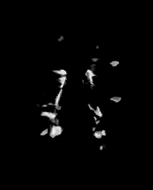
\includegraphics[height=4cm]{figures/lesions.png}};
\end{scope}

% 1-channel input

\foreach \x in {20} {
\begin{scope}[xshift=\x pt]
\draw[fill=white, fill opacity=0.75]
  (0,0) coordinate(A\x) -- ++(90:4) coordinate (B\x) -- ++(30:2) coordinate
  (C\x) -- ++(-90:4) coordinate (D\x) -- cycle;
  
\draw (0,3)
   ++(30:0.25) \ifnum\x=20 coordinate (a1) \else -- +(0:10pt) +(0:0) \fi
-- ++(90:0.5)  \ifnum\x=20 coordinate (b1) \else -- +(0:10pt) +(0:0) \fi
-- ++(30:0.25) \ifnum\x=20 coordinate (c1) \else -- +(0:10pt) +(0:0) \fi
-- ++(-90:0.5) \ifnum\x=20 coordinate (d1) \else -- +(0:10pt) +(0:0) \fi
-- ++(210:0.25);
\end{scope}
}

\node[pin=30:Visible\\ units] at ($(C20)!0.25!(D20)$) {};

% Transition

\draw ($(a1)!0.5!(c1)$) ++(55pt,-5pt) coordinate (e1);
\draw (a1) -- (e1);
\draw (b1) -- (e1);
\draw (c1) -- (e1);
\draw (d1) -- (e1);

% First layer hidden units

\foreach \x in {80,85,90,95,100,105} {
\begin{scope}[xshift=\x pt,yshift=1.5cm,scale=0.5]
\draw[fill=white, fill opacity=0.75]
  (0,0) coordinate(A\x) -- ++(90:4) coordinate (B\x) -- ++(30:2) coordinate
  (C\x) -- ++(-90:4) coordinate(D\x) -- cycle;
   
\draw (0,2.5)
   ++(30:0.25) \ifnum\x=105 coordinate (a2) \else -- +(0:10pt) +(0:0) \fi
-- ++(90:1)    \ifnum\x=105 coordinate (b2) \else -- +(0:10pt) +(0:0) \fi
-- ++(30:0.5)  \ifnum\x=105 coordinate (c2) \else -- +(0:10pt) +(0:0) \fi
-- ++(-90:1)   \ifnum\x=105 coordinate (d2) \else -- +(0:10pt) +(0:0) \fi
-- ++(210:0.5);
\end{scope}
}

\draw[decorate,decoration={brace,raise=4pt,mirror}]
%(A80) --node[below=8pt] {$N = 32$} (A80-|D105);
(A80) --node[below=8pt] {$N = 32$} (A80-|D105);

\draw ($(a2)!0.5!(c2)$) ++(0:38pt) coordinate (e2);
\draw (a2) -- (e2);
\draw (b2) -- (e2);
\draw (c2) -- (e2);
\draw (d2) -- (e2);

\node[pin=30:Hidden\\ units] at ($(C105)!0.2!(D105)$) {};

% Second layer hidden units

\foreach \x in {145, 150, ..., 175, 180} {
\begin{scope}[xshift=\x pt,yshift=2.25cm,scale=0.25]
\draw[fill=white, fill opacity=0.75]
  (0,0) coordinate(A\x) -- ++(90:4) coordinate (B\x) -- ++(30:2) coordinate
  (C\x) -- ++(-90:4) coordinate(D\x) -- cycle;
\draw (0,1.75)
   ++(30:0.25) \ifnum\x=180 coordinate (a3) \else -- +(0:20pt) +(0:0) \fi
-- ++(90:2)    \ifnum\x=180 coordinate (b3) \else -- +(0:20pt) +(0:0) \fi
-- ++(30:1)    \ifnum\x=180 coordinate (c3) \else -- +(0:20pt) +(0:0) \fi
-- ++(-90:2)   \ifnum\x=180 coordinate (d3) \else -- +(0:20pt) +(0:0) \fi
-- ++(210:1);
\end{scope}
}

\draw[decorate,decoration={brace,raise=4pt,mirror}]
(A145) --node[below=8pt] {$N = 64$} (A145-|D180);

\draw ($(a3)!0.5!(c3)$) ++(0:18pt) coordinate (e3);
\draw (a3) -- (e3);
\draw (b3) -- (e3);
\draw (c3) -- (e3);
\draw (d3) -- (e3);

% Third layer hidden units

\foreach \x in {200, 205, ..., 240} {
\begin{scope}[xshift=\x pt,yshift=2.625cm,scale=0.125]
\draw[fill=white, fill opacity=0.75]
  (0,0) coordinate(A\x) -- ++(90:4) coordinate (B\x) -- ++(30:2) coordinate
  (C\x) -- ++(-90:4) coordinate(D\x) -- cycle;
\end{scope}
}

%\node[rotate=90] at(270pt,2.75cm) {Serialize hidden units};

% Forth layer visible units (dense)

\begin{scope}[xshift=280pt, yshift=2.75cm]
\foreach \x/\y in {0/-2, 1/-1.5, 2/-1, 3/-0.5, 4/0, 5/0.5, 6/1, 7/1.5, 8/2} {
  \node[circle, draw] (V\x) at (0,\y) {};
}
\end{scope}

\draw[shorten >=10pt,shorten <=10pt,dashed] (A240)--(V0.south west);
\draw[shorten >=10pt,shorten <=10pt,dashed] (A240|-C240)--
%node[label=120:Vectorize\\ hidden units] {}
(V8.north west);

\draw[decorate,decoration={brace,raise=4pt,mirror}]
(A200) --node[below=8pt,fill=white] {$N = 32$} (A200-|D240);

%\node[rotate=90,fill=white,align=center] at(270pt,2.75cm) {Serialize\\ hidden
%units};

% Forth layer hidden units (dense)

\begin{scope}[xshift=320pt, yshift=2.75cm]
\foreach \x/\y in {0/-1, 1/-0.5, 2/0, 3/0.5, 4/1} {
  \node[circle, draw] (H\x) at (0,\y) {};
}
\end{scope}

\foreach \x in {0, ..., 8} {
  \foreach \y in {0, ..., 4} {
    \draw[very thin] (V\x)--(H\y);
  }
}

% Fifth layer hidden units (distribution parameters)

\begin{scope}[xshift=360pt, yshift=2.75cm]
\foreach \x/\y in {1/0.25, 2/-0.25} {
  \node[circle, draw, label=0:$L_\x$] (L\x) at (0,\y) {};
}
\end{scope}

\foreach \x in {0, ..., 4} {
  \foreach \y in {1,2} {
    \draw[very thin] (H\x)--(L\y);
  }
}
\end{scope}

%%%%%%%%%%%%%%
% Joint layer
%%%%%%%%%%%%%%

% yshift = 2.75 - 6/2 = -0.25

\begin{scope}[xshift=380pt, yshift=-0.25cm]
\foreach \x/\y in {1/-0.75, 2/-0.25, 3/0.25, 4/0.75} {
  \node[circle, draw, label=0:$J_\x$] (J\x) at (0,\y)
  {}; }
\end{scope}

\foreach \x in {0, ..., 4} {
  \foreach \y in {1, ..., 4} {
    \draw[very thin] (h\x)--(J\y);
    \draw[very thin] (H\x)--(J\y);
  }
}

\node[yshift=-15pt, fill=white, inner sep=3pt] at (h0) {$N = 16$};

\draw[decorate,decoration={brace,raise=30pt,mirror}] (V0.south-|J1)
--node[dbnlabel, below=35pt, sloped] {Joint DBN} (v8.north-|J1);

\end{tikzpicture}
\caption{DBN models used for discovering patterns.}
\end{figure}

The probability density function $p(u)$ is modeled by a deep belief network
(DBN) \cite{Hinton2006b}, a generative probabilistic graphical model consisting
of one layer of observed random variables (visible units) and multiple layers of
latent random variables (hidden units). In a DBN, each pair of adjacent layers
of random variables form a restricted Boltzmann machine (RBM). The first RBM
receives the displacement fields of a training set as input and reduces the
dimensionality of each field by discovering patterns of similarity that are
common within groups of displacement fields. Each subsequent RBM receives the
hidden unit activations of the previous RBM as input, thus learning successively
more complex and abstract patterns from the training data. In particular, we use
a DBN with three strided convolutional RBMs\footnote{The three sconvRBMs have
stride sizes of \num{2x2x1}, \num{2x2x2}, \num{1x1x1}, filter sizes of
\num{10x10x7}, \num{10x10x10}, \num{3x5x3}, and 32, 64, 32 filters,
respectively.} (sconvRBMs) and two dense RBMs \cite{Hinton2010} with 16 and 2
hidden units, respectively. In the following, we will briefly review the
sconvRBM, as this model is less often described in the literature, followed by
how the visible and hidden units of the DBN relate to displacement fields and
displacement field distribution parameters. A sconvRBM is a type of RBM in which
the probabilistic relationships between the visible and hidden units are
expressed in terms of strided convolutions, a type of convolution that shifts
the filter kernel as a sliding window with a step size or stride $s > 1$. Due to
the much smaller number of trainable parameters compared to dense RBMs,
sconvRBMs are best suited for learning low- to mid-level features from very
high-dimensional data. Compared to other more commonly used convolution-based
RBMs \cite{Lee2009}, an advantage of sconvRBMs is that inference is invertible,
which allows the reconstruction of the visible units from the hidden unit
activations. In our application, this would allow for the reconstruction of
deformation fields from distribution parameters. The complete morphology DBN can
be trained layer-by-layer by training each RBM individually using contrastive
divergence \cite{Hinton2006b}. Once the parameters of the DBN have been learned
from training data, we can use the model for inference. Let
$\vect{v}_{\text{d},1}, \dotsc, \vect{v}_{\text{d},5}$, $\vect{h}_{\text{d},1},
\dotsc, \vect{h}_{\text{d},5}$, and $\thetas_{\text{d},1}, \dotsc,
\thetas_{\text{d},5}$ denote the visible units, hidden units, and parameters,
respectively, of each RBM of the morphology DBN. Then, for a given displacement
field $u_n$, we can calculate the parameters $(D_1, \dotsc)^T$ of $u \sim p(u
\mid D_1, \dotsc)$ with
\begin{align} 
\label{eq:inferd}
(D_1, \dotsc)^T &= \E[D_1, \dotsc \mid u_n] = \E[\vect{h} \mid
\vect{v}_{\text{d},5}, \thetas_{\text{d},5}] \\
\label{eq:inferv}
\vect{v}_{\text{d},i+1} &= \E[\vect{h} \mid \vect{v}_{\text{d},i},
\thetas_{\text{d},i}]
\end{align}
where $i \in [1,4]$ and $\vect{v}_{\text{d},1} = u_n$. Inversely, the mean
displacement field $\bar{u}$ given the distribution parameters can be calculated
by
\begin{align}
\label{eq:inferu}
\bar{u} &= \E[u \mid D_1, \dotsc] = \E[\vect{v} \mid \vect{h}_{\text{d},1},
\thetas_{\text{d},1}] \\
\label{eq:inferh}
\vect{h}_{\text{d},i} &= \E[\vect{v} \mid \vect{h}_{\text{d},i+1},
\thetas_{\text{d},i+1}]
\end{align}
where $i \in [1,4]$ and $\vect{h}_{\text{d},5} = (D_1,\dotsc)^T$.

The input into our lesion model is a set of 3D binary lesion masks $l_n
\in I$, which have been created from T2-weighted (T2w) and PD-weighted (PDw) MRIs by experts using a semi-automatic method. All lesion masks are spatially aligned to MNI space using
the transformations as calculated for the corresponding T1w images. Analogous to
the morphology model, we assume that lesion masks $l_n$ are samples from
an unknown distribution $l_n \sim p(l \mid L_1, \dotsc)$ that can be
parameterized by only relatively few parameters $(L_1, \dotsc)^T$. The task of finding lesion
patterns is to discover the underlying probability density function $p(l \mid
L_1, \dotsc)$, where the parameters $(L_1, \dotsc)^T$ represent patterns of
variability of MS lesions. Similar to the morphology DBN, the lesion DBN
consists of three sconvRBMs\footnote{The three sconvRBMs have stride sizes of
\num{4x4x2}, \num{2x2x2}, \num{2x2x2}, filter sizes of \num{20x20x10},
\num{14x14x10}, \num{10x14x6}, and 32, 64, 64 filters, respectively.} and two
dense RBMs with 16 and 2 hidden units, respectively.
However, we modified the energy function of the sconvRBMs to account for the
sparse activation of MS lesion masks. Large black regions without local
structure can lead to random activations of the hidden units and consequently
the learning of random filters. To overcome this problem, we propose to
incorporate a region of interest (ROI) term into the energy equation of the
sconvRBM, which allows constraining the filter learning process to a given ROI.
This can be achieved by element-wise multiplication of the visible and hidden
units with a binary mask, which sets the visible and hidden units outside of the
ROI to zero, thereby removing their contribution to the energy of the model.
The ROI was chosen to include all white matter lesions from the training set.
Similarly to the morphology model, for a trained lesion DBN and a given lesion
mask $l_n$, we can calculate the parameters $(L_1,\dotsc)^T$ of $l_n \sim
p(l\mid L_1,\dotsc)$ in the same manner as in \eqref{eq:inferd} and
\eqref{eq:inferv}. Likewise, the mean lesion configuration $\bar{l}$ given the
distribution parameters $(L_1,\dotsc)^T$ can be calculated in the same manner as
in \eqref{eq:inferu} and \eqref{eq:inferh}.

To discover concurring patterns of morphology and lesion distribution, we
combine the morphology DBN and the lesion DBN to form the joint DBN, which
defines the joint distribution $p(u, l \mid J_1, \dotsc)$. The joint DBN
consists of two pathways, each corresponding to the first 4 layers of the
morphology and lesion DBNs, respectively, and a 5th RBM layer with 4 hidden
units, which replaces the 5th layer of the individual DBNs and combines the
hidden unit activations of the 4th layer RBMs. That is, the 5th RBM defines the
joint probability $p(\vect{v}_\text{j}, \vect{h}_\text{j} \mid
\thetas_\text{j})$, where $\vect{v}_\text{j} = (\vect{h}_{\text{d},4}^T,
\vect{h}_{\text{l},4}^T)^T$ and $\vect{h}_\text{j} = (J_1, \dotsc)^T$ are the
modes of variability of morphological and lesion distribution changes.


\subsection{Evaluation}

The proposed method was evaluated on a dataset from an MS clinical trial of 474
secondary progressive MS patients. For each subject, the dataset contains one
T1w, T2w, and PDw MRI with a resolution of \num{256x256x50} voxels and a voxel
size of \SI{0.937x0.937x3.000}{\milli\meter}. The main preprocessing steps
included rigid registration, brain extraction, intensity normalization, and
background cropping. We then trained the 3 DBN models as described in
Sect.~\ref{sec:method}.

The invertibility of our model allows the reconstruction of images from the
distribution parameters to visualize the discovered patterns of variability.
Figure~\ref{fig:deformations} shows axial slices from volumes generated from the
2-parameter morphology model $p(u \mid D_1, D_2)$. To generate these images, we
calculated the mean displacement fields for varying values of $D_1$ and $D_2$
to span the range of variability represented by the
training set and applied the inverse deformations to the ICBM 152 template
image. The most apparent morphological variability captured by the morphology
model is ventricular enlargement for $D_1$ and overall brain size for $D_2$.
Figure~\ref{fig:lesions} shows axial slices from the mean lesion configurations
$\E[l \mid L_1, L_2]$ for varying lesion distribution parameters. An increase of
$L_2$ visually correlates with an increase of lesions specifically around the
ventricles, whereas an increase of $L_1$ visually correlates with an increase of
lesions in the entire white matter.

\begin{figure}[tb]
\newlength{\subfigwidth}
\setlength{\subfigwidth}{0.232\textwidth}
\centering
\subfloat[Morphology manifold] {
\label{fig:deformations}
\begin{tikzpicture}
\tikzstyle{every node}+=[font=\scriptsize]
\node
(manifold){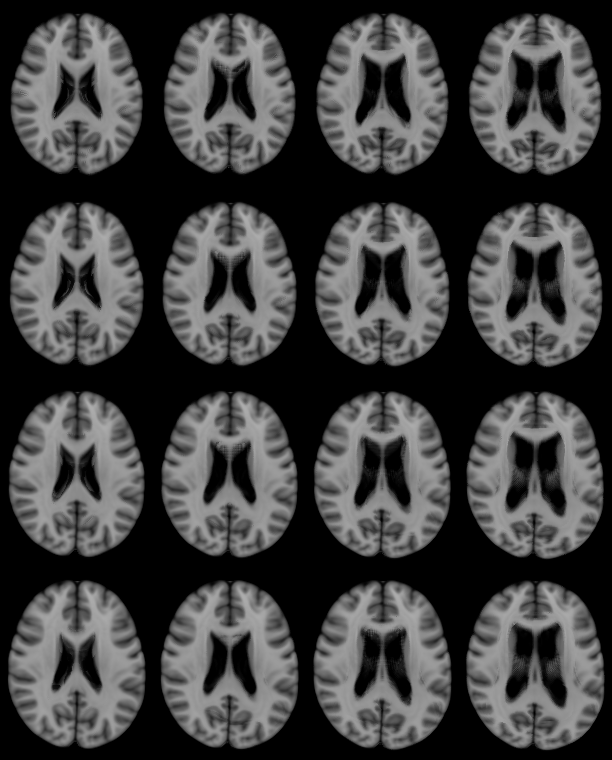
\includegraphics[width=\subfigwidth]{figures/MICCAI2014_warps_t1_dark}};

\draw[->] (manifold.south west)--node[below=4pt,inner sep=0] {$D_1$}
(manifold.south east);
\draw[->] (manifold.south west)--node[above=4pt,sloped,inner sep=0] {$D_2$}
(manifold.north west);

\end{tikzpicture}
}
\subfloat[Lesion manifold] {
\label{fig:lesions}
\begin{tikzpicture}
\tikzstyle{every node}+=[font=\scriptsize]
\node
(manifold){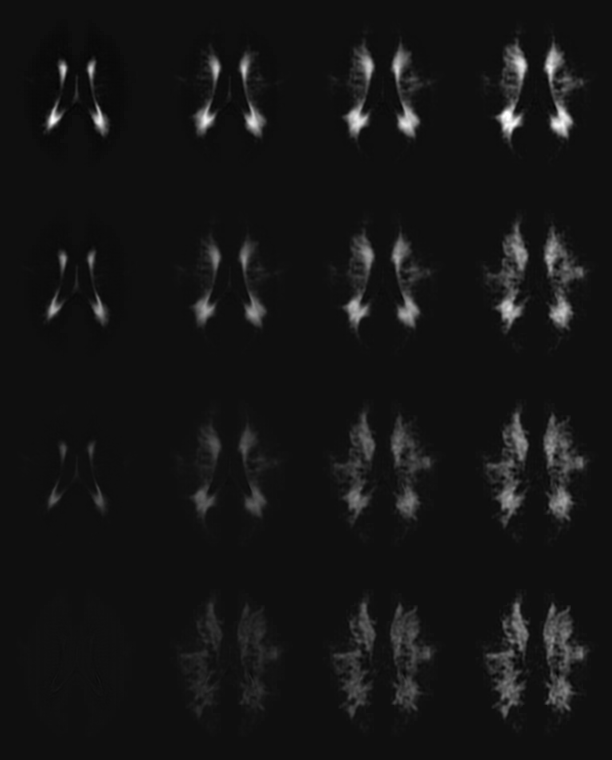
\includegraphics[width=\subfigwidth]{figures/MICCAI2014_p442_d0_full_h16-2}};

\draw[->] (manifold.south west)--node[below=4pt,inner sep=0] {$L_1$} (manifold.south east);
\draw[->] (manifold.south west)--node[above=4pt,sloped,inner sep=0] {$L_2$}
(manifold.north west);

\end{tikzpicture}
}%
\subfloat[Joint manifold] {
\label{fig:joint}
\begin{tikzpicture}
\tikzstyle{every node}+=[font=\scriptsize]

\node[align=left,fill=black,inner sep = 0pt] (manifold1) {
  \mbox{}\\[2pt]
  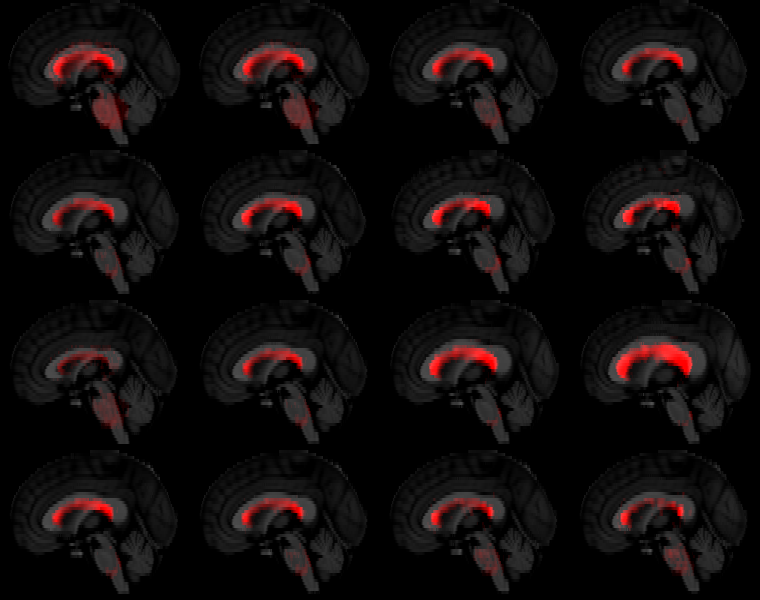
\includegraphics[trim=0 340 0 0,clip,width=\subfigwidth]
    {figures/MICCAI2014_full_rl1_h4_sag}\\[8.5pt]
  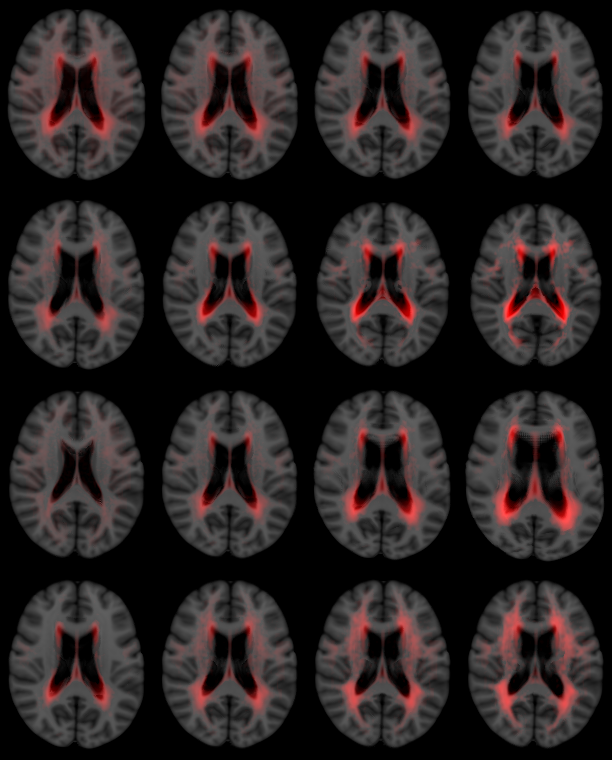
\includegraphics[trim=0 0 0 150,clip,width=\subfigwidth]
    {figures/MICCAI2014_full_rl1_h4}
};
\node[fit=(manifold1)] (manifold) { };

\foreach \x/\y in {0.125/1, 0.375/2, 0.625/3, 0.875/4} {
  \node[left,inner sep=0pt] at ($(manifold.north west)!\x!(manifold.south
  west)$) {$J_\y$}; }

\draw[->] (manifold.south west)--node[below=4pt,inner sep=0] {$J_x$} (manifold.south east);

\end{tikzpicture}
} \caption{Slices from generated volumes from the (a) morphology, (b) lesion,
and (c) joint model. The morphology model captures ventricular
enlargement ($D_1$) and decrease in brain size ($D_2$) as the main modes of
variation. For the lesion model, $L_1$ captures an increase in lesion load
throughout the WM, while $L_2$ captures primarily periventricular lesion load
variations. The parameters of the joint model capture combinations
of the variability found in the individual models.}
\label{fig:samples}
\end{figure}

To visualize concurring patterns of morphology and lesion distribution, we
sampled images from the joint model $p(u, l \mid J_1, \dotsc, J_4)$ as shown in
Fig.~\ref{fig:joint}. The images are deformed template images with superimposed
lesion masks. For each row, we varied only one distribution parameter and set
the remaining parameters to their mean values. Of the 4 parameters, $J_3$
visually corresponds most closely to the ``classic'' progression of MS
pathology, with an enlargement of the ventricles paired with an increased
periventricular lesion load. The parameters $J_2$ and $J_4$ also reveal
simultaneous morphological and lesion variations that are visible on the chosen
axial slice. For $J_1$, a lesion pattern is not obvious unless the images are
viewed sagittally, which reveals changes in lesion load in the pons.

\begin{table}[tb]
\centering 
\small
\caption{Pearson correlations $r$ of clinical
scores with distribution parameters of the morphology model ($D_1$, $D_2$),
lesion model ($L_1$, $L_2$), joint model ($J_1$, $J_2$, $J_3$, $J_4$),
normalized brain volume (nBV), and lesion load (LL). The level of
statistical significance is indicated by the number of asterisks (* $p < 0.05$,
** $p < 0.01$, *** $p < 0.001$).
}

%\NewDocumentCommand{\sym}{m}{#1}

\label{tab:correlations}
\sisetup{
  round-mode = places,
  round-precision = 3,
  exponent-product = \cdot,
  detect-weight=true,
  detect-inline-weight=math,
  tight-spacing = false,
  table-align-text-post = false
}%

\def\tabspace{14pt}

\begin{tabular}{c@{\hspace{\tabspace}}c%
@{\hspace{\tabspace}}S[table-format=2.5]%
@{\hspace{\tabspace}}S[table-format=2.6]
@{\hspace{\tabspace}}S[table-format=2.6]
@{\hspace{\tabspace}}S[table-format=2.6]}
\toprule
 &  & {T25W} & {9-HPT} & {PASAT} & {MSFC} \\
 \midrule
 
\multirow{4}*{\minitab[c]{Individual\\ models}}
 & $D_1$ &
\bfseries -0.128976787246536** & -0.214588136146619*** & -0.282044527648157*** &
-0.314633263656368*** \\
 & $D_2$ & 0.0870255979372807 & 0.115835195120173* & 0.08923208653141 &
0.138616500875685** \\
& $L_1$ & -0.0581629511079419 & -0.231012897586838*** & -0.391822792658197*** &
-0.366992537420278*** \\
& $L_2$ & -0.091057480388512 & \bfseries -0.354478789398171*** &
\bfseries -0.426543205964196*** & \bfseries -0.463860459137063*** \\
\addlinespace
\multirow{4}*{\minitab[c]{Joint\\ model}}
 & $J_1$ & 0.107219513748914* & 0.285812780188632*** & 0.336253511146623*** &
0.378889115681159*** \\
 & $J_2$ & -0.037731447660239 & -0.209982769437628*** & -0.226800472678912***
& -0.255585426983655*** \\
& $J_3$ & \bfseries -0.117780586822506* & \bfseries -0.369169927947271*** &
\bfseries -0.452556545437486*** & \bfseries -0.494130959187706*** \\
& $J_4$ & -0.0491209563011896 & -0.205764640863705*** & -0.382954826511733*** &
-0.345529171963859*** \\
\addlinespace
\multirow{2}*{\minitab[c]{Imaging\\ biomarkers}}
 & nBV & 0.0530068558456253 & 0.143905618421747** & 0.246833144651129***
& 0.234774254053599*** \\
 & LL & -0.073681606595365 & \bfseries -0.286360084620956*** &
\bfseries -0.399646128024074*** & \bfseries -0.406222020153583*** \\
  
 \bottomrule
\end{tabular}

\end{table}

To evaluate the potential of the distribution parameters to reveal clinically
relevant information, we have calculated the Pearson correlation $r$ of the
clinical MS Functional Composite (MSFC) \cite{Fischer1999} and its components
(Timed 25-Foot Walk, T25W; 9-Hole Peg Test, 9-HPT; Paced Auditory Serial
Addition Test, PASAT) with the distribution parameters and two established MS
imaging biomarkers (normalized brain volume, nBV, as calculated by SIENAX
\cite{Smith2002} and lesion load, LL). The results of the correlation tests are
summarized in Table~\ref{tab:correlations}. In the individual models, all
parameters correlate significantly with 9-HPT, PASAT, and MSFC, except for $D_2$
with PASAT. The morphology parameter $D_1$ correlates more strongly with these
scores than nBV, as does the lesion parameter $L_2$ than LL. For T25W, $D_1$
shows a modest but significant correlation while nBV does not. In the joint
model, all parameters correlate significantly with 9-HPT, PASAT, and MSFC, with
$J_3$ being particularly strong. The parameter $J_3$ shows stronger correlations
than nBV or LL for all clinical scores, including a modest significant
correlation to T25W, which is not shown by nBV nor LL. The significant
correlation between $J_1$ and T25W is particularly interesting because the
lesion changes modeled by $J_1$ occur in the pons, which is known to be of
clinical significance for mobility. Overall, the learned parameters correlate
better than the established imaging biomarkers.

\begin{figure}[tb]
\centering
\subfloat[Morphological changes] {
\begin{tikzpicture} 
\tikzstyle{every node}=[font=\scriptsize]
\node[align=left,inner sep=0] (images) {
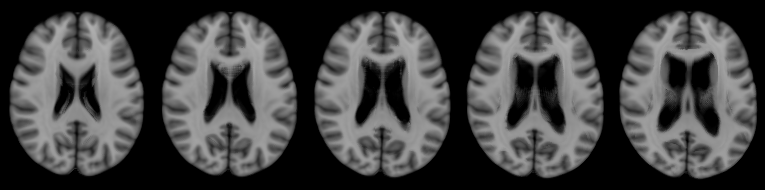
\includegraphics[width=0.47\textwidth]{figures/MICCAI2014_full_rl1_h4_MSFC_nolesion}
\\

\includegraphics[width=0.47\textwidth]{figures/MICCAI2014_full_rl1_h4_MSFC_sag_nolesion}
};
\foreach \x/\y in {0.1/1.5, 0.3/0, 0.5/-1.5, 0.7/-3, 0.9/-4.5} {
  \node[above=2pt] at ($(images.north west)!\x!(images.north east)$) {\y}; }
\end{tikzpicture}
}
\subfloat[Lesion changes] {
\begin{tikzpicture}
\tikzstyle{every node}=[font=\scriptsize] 
\node[align=left,inner sep=0] (images) {
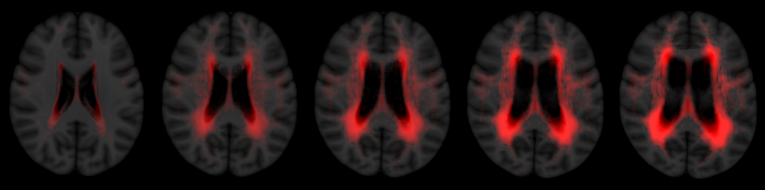
\includegraphics[width=0.47\textwidth]{figures/MICCAI2014_full_rl1_h4_MSFC} \\
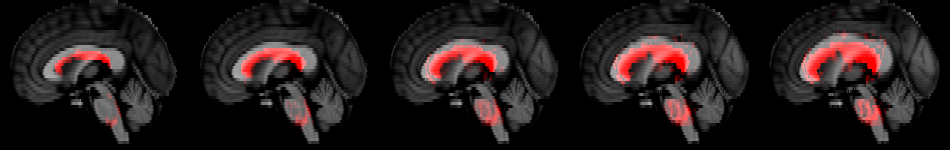
\includegraphics[width=0.47\textwidth]{figures/MICCAI2014_full_rl1_h4_MSFC_sag}
};
\foreach \x/\y in {0.1/1.5, 0.3/0, 0.5/-1.5, 0.7/-3, 0.9/-4.5} {
  \node[above=2pt] at ($(images.north west)!\x!(images.north east)$) {\y};
}
\end{tikzpicture}
}
\caption{Axial (top row) and mid-sagittal (bottom row) slices of volumes
representing the spectrum of MSFC scores from \num{1.5} to \num{-4.5}. A
decrease in MSFC shows the classic pattern of MS pathology.}
\label{fig:msspectrum}
\end{figure}

Another benefit of our model is the ability to visualize the progression of a
``mean'' secondary progressive MS brain along a range of MSFC scores.
To demonstrate, we trained 4 independent linear models to predict the
distribution parameters $J_1, \dotsc, J_4$ given the MSFC ($J_i = a_i +
b_i\text{MSFC}$). Figure~\ref{fig:msspectrum} shows the axial (top row) and
mid-sagittal (bottom row) slices of generated images representing the range of
MSFC scores from \num{1.5} to \num{-4.5}. Consistent with previous results, a
decrease in MSFC visually correlates with an increase in the size of the
ventricles, an increase in periventricular lesions, and an increase in lesions
in the pons region.

\section{Discussion}

Potentially follow up with a discussion where I can discuss related approaches
that came afterwards and what needs to be done.

\chapter{Medical Image Segmentation}

\begin{itemize}
\item 
Start with general MS lesion segmentation
literature review.
\item What are the challenges and how could deep learning help to
overcome them?
\item Then literature using deep learning for segmentation.
Patch-based approaches for lesion segmentation, even if not MS lesions.
\item More recent approach are fully convolutional. Then explain my method
including the evaluation.
\end{itemize}

% TODO: Take MS motivation out into a separate MS part

Multiple sclerosis (MS) is an inflammatory and demyelinating disease of the
central nervous system with pathology that can be observed in vivo by magnetic
resonance imaging (MRI). MS is characterized by the formation of lesions,
primarily visible in the white matter on conventional MRI. Imaging biomarkers
based on the delineation of lesions, such as lesion load and lesion count, have
established their importance for assessing disease progression and treatment
effect. However, lesions vary greatly in size, shape, intensity and location,
which makes their automatic and accurate segmentation challenging.

\section{Related Work}

\subsection{MS Lesion Segmentation Methods}

Many automatic methods have been proposed for the segmentation of MS
lesions over the last two decades \citep{garcia2013}, which can be
classified into unsupervised and supervised methods. Unsupervised methods do not
require a labeled data set for training. Instead, lesions are identified as an
outlier class using, e.g., clustering methods
\citep{souplet2008,shiee2010} or generative models \citep{weiss2013}. In
addition to modelling MS lesions as a separate cluster, Lesion-TOADS
\citep{shiee2010} employs a topological and a statistical atlas to
produce a topology-preserving segmentation. Current supervised approaches
typically start with a large set of features, either predefined by the user
\citep{geremia2010} or gathered in a feature extraction step such as by deep
learning\citep{yoo2014}, which is followed by a separate training step with
labeled data to determine which set of features are the most important for
segmentation in the particular domain.
% For example, Yoo et al. \citep{yoo2014} proposed performing unsupervised
% learning of domain-specific features from image patches from unlabelled data
% using deep learning.
A recent breakthrough for automatic segmentation using deep learning comes from
the domain of cell membrane segmentation, in which Ciresan et al.
\citep{Ciresan2012} proposed to classify the centers of image patches directly
using a convolutional neural network (CNN) \citep{LeCun1998} without a dedicated
feature extraction step. Instead, features are learned indirectly within the
lower layers of the neural network during training, while the higher layers can
be regarded as performing the classification, which allows the learning of
features that are specifically tuned to the segmentation task. However, the time
required to train patch-based methods can make the approach infeasible when the
size and number of patches are large.

% TODO: can I add numerical values to it? Mostly my personal experience.

\subsection{Patch-based approaches using Deep Learning}

% TODO: Have to put Yoo and Ciresan here

\subsection{Fully Convolutional Approaches}

Recently, different CNN architectures
\citep{ronneberger2015,brosch2015,kang2014} have been proposed that are able
to feed through entire images, which removes the need to select representative
patches, eliminates redundant calculations where patches overlap, and therefore
scales up more efficiently with image resolution. Kang et al. introduced the
fully convolutional neural network (fCNN) for the segmentation of crowds in
surveillance videos \citep{kang2014}. However, fCNNs produce segmentations
of lower resolution than the input images due to the successive use of
convolutional and pooling layers, both of which reduce the dimensionality.
To predict segmentations of the same resolution as the input images, we recently
proposed using a 3-layer convolutional encoder network (CEN) \citep{brosch2015}
for MS lesion segmentation. The combination of convolutional \citep{LeCun1998}
and deconvolutional \citep{zeiler2011} layers allows our network to produce
segmentations that are of the same resolution as the input images. 

Another limitation of the traditional CNN is the trade-off between localization
accuracy, represented by lower-level features, and contextual information,
provided by higher-level features.
%
Ronneberger et al. \citep{ronneberger2015}
%
% found that increasing the depth of the
% CNN, and thereby increasing the size of the receptive field of a segmented voxel,
% increases the abstraction from the input data, which makes the segmentation
% method more robust to anatomical and intensity variations. They
%
proposed an 11-layer u-shaped network architecture called u-net,
% which leverages high-level and low-level features in order to predict
% segmentations that are both robust and accurate.
composed of a traditional contracting path (first half of the u), but augmented
with an expanding path (last half of the u), which replaces the pooling layers
of the contracting path with upsampling operations. To leverage both high- and
low-level features, shortcut connections are added between corresponding layers
of the two paths.
However,
% the successive application of convolutional, pooling, and
% unpooling layers reduces the size of the predicted segmentation by the size of
% the receptive field. This requires special handling of the border regions and
% limits the maximum size of the receptive field.
upsampling cannot fully compensate for the loss of resolution, and special
handling of the border regions is still required.

\section{Method}

We propose a new convolutional network architecture that combines the advantages
of a CEN \cite{brosch2015} and a u-net \cite{ronneberger2015}. Our network is
divided into two pathways, a traditional convolutional pathway, which consists
of alternating convolutional and pooling layers, and a deconvolutional pathway,
which consists of alternating deconvolutional and unpooling layers and predicts
the final segmentation. Similar to the u-net, we introduce shortcut connections
between layers of the two pathways. In contrast to the u-net, our network uses
deconvolution instead of upsampling in the expanding pathway and predicts
segmentations that have the same resolution as the input images and therefore
does not require special handling of the border regions.

\subsection{Solving Segmentation as an Optimization Problem}

In this paper, the task of segmenting MS lesions is defined as finding a
function $s$ that maps multi-modal images $I$, e.g., $I = (I_\text{FLAIR},
I_\text{T1})$, to corresponding lesion masks $S$. Given a set of
training images $I_n$, $n \in \N$, and corresponding segmentations $S_n$, we
model finding an appropriate function for segmenting MS lesions as an
optimization problem of the following form
\begin{equation}
\hat{s} = \arg \min_{s \in \mathcal{S}} \sum_n E(S_n, s(I_n)),
\label{eq:segprob}
\end{equation}
where $\mathcal{S}$ is the set of possible segmentation functions, and $E$ is an
error measure that calculates the dissimilarity between ground truth
segmentations and predicted segmentations.

\subsection{Model Architecture}

The set of possible segmentation functions, $\mathcal{S}$, is modeled by the
convolutional encoder network with shortcut connections (CEN-s) illustrated in
Fig.~\ref{fig:network}. A CEN-s is a type of convolutional neural network (CNN)
\cite{LeCun1998} that is divided into two interconnected pathways, the
convolutional pathway and the deconvolutional \cite{zeiler2011} pathway. The
convolutional pathway consists of alternating convolutional and pooling layers.
The input layer of the convolutional pathway is composed of the image voxels
$x^{(0)}_i(\vect{p})$, $i \in [1, C]$, where $i$ indexes the modality or input
channel, $C$ is the number of modalities or channels, and $\vect{p} \in \N^3$
are the coordinates of a particular voxel. The convolutional layers
automatically learn a feature hierarchy from the input images. A convolutional
layer is a deterministic function of the following form
\begin{equation}
x^{(l)}_j = \max \Bigg(0, \sum_{i=1}^C\tilde{w}^{(l)}_{\text{c},ij}*x^{(l-1)}_i
+ b^{(l)}_j\Bigg),
\end{equation}
where $l$ is the index of a convolutional layer, $x^{(l)}_j$, $j \in [1,F]$,
denotes the feature map corresponding to the trainable convolution filter
$w^{(l)}_{\text{c},ij}$, $F$ is the number of filters of the current layer,
$b^{(l)}_j$ are trainable bias terms, $*$ denotes valid convolution, and
$\tilde{w}$ denotes a flipped version of $w$. A convolutional layer is followed
by an average pooling layer \cite{scherer2010} that halves the number
of units in each dimension by calculating the average of each block of
\num{2x2x2} units per channel.

\begin{figure}[tb]
\centering
\begin{tikzpicture}[
  node distance=0.75cm and 0.65cm,
  font=\footnotesize,
  conv/.style={green!60!black,-latex,thick},
  conv2/.style={green!60!black,latex-latex,thick},
  pooling/.style={-latex,red!60!black,thick},
  deconv/.style={-latex,blue!60!black,thick},
  unpooling/.style={-latex,brown!60!black,thick},
  channel/.style args={#1 and #2}{draw, fill=lightgray, inner sep=0pt,
      minimum width=#1, minimum height=#2}
]

% \tikzstyle{channel}=[draw,minimum width=64pt,fill=lightgray,inner
% sep=0pt,minimum height=#1]

% Network

\begin{scope}[local bounding box=network]
\node[channel=64pt and 3pt,pin=270:Input images] (inputs) {};
\node[channel=60pt and 16pt,above=of inputs] (clayer1) {};
\node[channel=30pt and 16pt,above=of clayer1] (pooling1) {};

\node[channel=64pt and 1pt,right=of inputs,pin=270:Segmentations] (outputs) {};
\node[channel=60pt and 16pt] (dlayer1) at (clayer1-|outputs) {};
\node[channel=30pt and 16pt,above=of dlayer1] (dpooling1) {};

\node[fit=(pooling1)(dpooling1),inner sep = 0pt] (pooling) {};
\node[channel=26pt and 16pt,above=of pooling] (clayer2) {};
\end{scope}

\draw[conv] (inputs)--node[left] {$w^{(1)}_\text{c}$} (clayer1);
\draw[pooling] (clayer1)--node[left] {} (pooling1);
\draw[conv] (pooling1)--node[left] {$w^{(3)}_\text{c}$} (clayer2);
\draw[deconv] (clayer2)--node[right=5pt] {$w^{(3)}_\text{d}$} (dpooling1);
\draw[unpooling] (dpooling1)--node[right] {} (dlayer1);
\draw[deconv] (dlayer1)--node[right] {$w^{(1)}_\text{d}$} (outputs);
\draw[deconv] (clayer1)--node[anchor=188,inner sep=10pt]
{$w^{(1)}_\text{s}$}(outputs);

% Part labels

\node[left=1pt of inputs] {$x^{(0)}$};
\node[left=1pt of clayer1] {$x^{(1)}$};
\node[left=1pt of pooling1] {$x^{(2)}$};
\node[left=1pt of clayer2] {$x^{(3)}$};

\node[right=1pt of outputs] {$y^{(0)}$};
\node[right=1pt of dlayer1] {$y^{(1)}$};
\node[right=1pt of dpooling1] {$y^{(2)}$};
\node[right=1pt of clayer2] {$y^{(3)}$};

% Layers

\draw[decorate,decoration={brace,raise=30pt}] (inputs.south west)
--node[left=35pt,align=center] (convl) {Convolutional\\ layer} (inputs.south
west|-clayer1.north west);

\draw[decorate,decoration={brace,raise=22pt}] (clayer1.south west)
--node[left=27pt,align=center] {Pooling\\ layer} (clayer1.south
west|-pooling1.north west);

\draw[decorate,decoration={brace,raise=25pt}] (pooling1.south west)
--node[left=30pt,align=center] {Convolutional\\ layer} (clayer2.north
west-|pooling1.south west);

\draw[decorate,decoration={brace,raise=30pt,mirror}] (outputs.south east)
--node[right=35pt,align=center] {Deconvolutional\\ layer with shortcut}
 (dlayer1.north east-|outputs.south east);

\draw[decorate,decoration={brace,raise=22pt,mirror}] (dlayer1.south east)
--node[right=27pt,align=center] {Unpooling\\ layer}
(dpooling1.north east-|dlayer1.south east);

\draw[decorate,decoration={brace,raise=25pt,mirror}] (dpooling1.south east)
--node[right=30pt,align=center] {Deconvolutional\\ layer}
(clayer2.north east-|dpooling1.south east);

% Legend

\begin{scope}[local bounding box=ghost,opacity=0]
\path[conv] node (conv) {convolution} [draw] (conv.west)
++(left:0.5)--++(right:0.5);

\path[pooling] node[right=0.8 of conv] (pool) {pooling} [draw] (pool.west)
++(left:0.5)--++(right:0.5);

\path[deconv] node[right=0.8 of pool] (dconv) {deconvolution} [draw]
(dconv.west) ++(left:0.5)--++(right:0.5);

\path[unpooling] node[right=0.8 of dconv] (unpool) {unpooling} [draw]
(unpool.west) ++(left:0.5)--++(right:0.5);
\end{scope}

\begin{scope}[local bounding box=ghost2,
    shift={($(network.south)-(ghost.north)$)},xshift=2pt,yshift=-7pt]

\path[conv] node (conv) {convolution} [draw] (conv.west)
++(left:0.5)--++(right:0.5);

\path[pooling] node[right=0.8 of conv] (pool) {pooling} [draw] (pool.west)
++(left:0.5)--++(right:0.5);

\path[deconv] node[right=0.8 of pool] (dconv) {deconvolution} [draw]
(dconv.west) ++(left:0.5)--++(right:0.5);

\path[unpooling] node[right=0.8 of dconv] (unpool) {unpooling} [draw]
(unpool.west) ++(left:0.5)--++(right:0.5);
\end{scope}

% Stack of CRBMs

\begin{scope}[local bounding box=dbn]
\node[channel=64pt and 3pt, left=6cm of inputs,pin=270:Input images] (rinputs)
{}; 
\node[channel=60pt and 16pt,above=of rinputs] (rclayer1) {};
\node[channel=30pt and 16pt,above=of rclayer1] (rpooling1) {};
\node[channel=26pt and 16pt,above=of rpooling1] (rclayer2) {};
\end{scope}

\draw[conv2] (rinputs)--node[left] {$\hat{w}^{(1)}$} (rclayer1);
\draw[pooling] (rclayer1)--node[right] {pooling} (rpooling1);
\draw[conv2] (rpooling1)--node[left] {$\hat{w}^{(2)}$} (rclayer2);

\node[left=1pt of rinputs] {$v^{(1)}$};
\node[left=1pt of rclayer1] {$h^{(1)}$};
\node[left=1pt of rpooling1] {$v^{(2)}$};
\node[left=1pt of rclayer2] {$h^{(2)}$};

\draw[decorate,decoration={brace,raise=5pt,mirror}] (rinputs.south east)
--node[right=10pt,align=center] (crbm) {convRBM$_1$} (rinputs.south
east|-rclayer1.north east);

\draw[decorate,decoration={brace,raise=5pt,mirror}] (rpooling1.south east)
--node[right=10pt,align=center] {convRBM$_2$} (rclayer2.north
east-|rpooling1.south east);

% \node[above=10pt of dbn,align=center] {Stack of Convolutional\\ Restricted
% Boltzmann Machines};
% \node[above=10pt of network] {Convolutional Encoder Network};

\node[above=15pt of dbn,align=center,font=\normalsize] {Pre-training};
\node[above=15pt of network,font=\normalsize] {Fine-tuning};

% \draw[->] (crbm.east|-dbn)-- node[above=2pt] {convert} 
% node[above,align=center]
% {$w_\text{c}^{(1)} = w^{(1)}$ \\
%  $w_\text{c}^{(2)} = w^{(2)}$ \\
%  $w_\text{d}^{(2)} = w^{(2)}$ \\
%  $w_\text{d}^{(1)} = 0.5w^{(1)}$ \\
%  $w_\text{s}^{(1)} = 0.5w^{(1)}$}
% (convl.west|-network);

%\draw (network.north west) rectangle (network.south east);
%\draw (ghost.north west) rectangle (ghost.south east);
%\draw (ghost2.north west) rectangle (ghost2.south east);

%\path[pooling] node (pool) at (-3,-1) {convolution};
%\draw[pooling] (conv.west) ++(left:0.5)--++(right:0.5);

%\draw[conv] (-3,-1)-- +(right:0.5) node[right] {convolution};
%\draw[pooling] (-0.5,-1)-- +(right:0.5) node[right] {pooling};
%\draw[deconv] (2,-1)-- +(right:0.5) node[right] {deconvolution};
%\draw[unpooling] (4.5,-1)-- +(right:0.5) node[right] {unpooling};

%\draw[pooling] (0,-1.5)-- +(right:0.5) node[right] {pooling};
%\draw[deconv] (0,-2)-- +(right:0.5) node[right] {deconvolution};
%\draw[unpooling] (0,-2.5)-- +(right:0.5) node[right] {unpooling};

\end{tikzpicture}

\caption{Pre-training and fine-tuning of the 7-layer convolutional encoder
network with shortcut that we used for our experiments. Pre-training is
performed on the input images using a stack of convolutional RBMs. The
pre-trained weights and bias terms are used to initialize a convolutional
encoder network, which is fine-tuned on pairs of input images, $x^{(0)}$, and
segmentations, $y^{(0)}$.}

\label{fig:network}
\end{figure}

The deconvolutional pathway consists of alternating deconvolutional and
unpooling layers with shortcut connections to the corresponding
convolutional layers. The first deconvolutional layer uses the extracted
features of the convolutional pathway to calculate abstract segmentation
features
\begin{equation}
y^{(L-1)}_i = \max\Bigg(0, \sum_{j=1}w^{(L)}_{\text{d},ij}\circledast
y^{(L)}_j + c^{(L-1)}_{i}\Bigg),
\end{equation}
where $y^{(L)} = x^{(L)}$, $L$ denotes the number of layers of the convolutional
pathway, $w^{(L)}_{\text{d},ij}$ and $c^{(L-1)}_i$ are trainable parameters of
the deconvolutional layer, and $\circledast$ denotes full convolution. Subsequent
deconvolutional layers use the activations of the previous layer
and corresponding convolutional layer to calculate more localized segmentation
features
% \begin{multline}
% y^{(l)}_i = \max\Bigg(0, \sum_{j=1}\Big(w^{(l+1)}_{\text{d},ij}\circledast
% y^{(l+1)}_j\\
% + w^{(l+1)}_{\text{s},ij}\circledast x^{(l+1)}_j\Big) +
% c^{(l)}_i\Bigg)
% \end{multline}
\begin{multline}
y^{(l)}_i = \max\Bigg(0, 
\sum_{j=1}w^{(l+1)}_{\text{d},ij}\circledast y^{(l+1)}_j\\
+ \sum_{j=1} w^{(l+1)}_{\text{s},ij}\circledast x^{(l+1)}_j +
c^{(l)}_i\Bigg),
\end{multline}
where $l$ is the index of a deconvolutional layer with shortcut, and
$w^{(l+1)}_{\text{s},ij}$ are the shortcut filter kernels connecting the
activations of the convolutional pathway with the activations of the
deconvolutional pathway. The last deconvolutional layer integrates the low-level
features extracted by the first convolutional layer with the high-level features
from the previous layer to calculate a probabilistic lesion mask
\begin{equation}
y^{(0)}_1 = \sigm\Bigg(\sum_{j=1}\Big(w^{(1)}_{\text{d},1j}\circledast
y^{(1)}_j +
w^{(1)}_{\text{s},1j}\circledast x^{(1)}_j\Big) + c^{(0)}_1\Bigg),
\end{equation}
where $\sigm(z)$ denotes the sigmoid function defined as $\sigm(z) = (1 +
\exp(-z))^{-1}, z \in \R$. To obtain a binary lesion mask from the probabilistic
output of our model, we chose a fixed threshold such that the mean Dice
similarity coefficient \cite{dice1945} is maximized on the training set
and used the same threshold for the evaluation on the test set.

\begin{comment}
The set of possible segmentation functions is modeled by the convolutional
encoder network illustrated in Fig.~\ref{fig:network}. Our network consists of
three layers: an input layer, a convolutional layer, and a deconvolutional
layer. The input layer is composed of the image voxels $x^{(1)}_i(\vect{p})$, $i
\in [1, C], C \in \N$, where $i$ indexes the modality, $C$ is the number of
modalities, and $\vect{p} \in \R^3$ are the coordinates of a particular voxel.
The convolutional layer automatically learns features from the input images. It
is a deterministic function of the following form
\begin{equation}
y^{(1)}_j = \max \left(0, \sum_{i=1}^{C}\tilde{w}^{(1)}_{ij}*x^{(1)}_i +
b^{(1)}_j\right)
\end{equation}
where $y^{(1)}_j, j \in [1, F], F \in \N$, denotes the feature map corresponding
to the trainable convolution filter $w^{(1)}_{ij}$, $F$ is the number of
filters, $b_j$ is a trainable bias term, $*$ denotes valid convolution, and
$\tilde{w}$ denotes a flipped version of $w$. The deconvolutional layer uses the
extracted features to calculate a probabilistic lesion mask as follows
\begin{equation}
y^{(2)} = \sigm\left(\sum_{j=1}^Fw^{(2)}_{j}\circledast x^{(2)}_j +
b^{(2)}\right)
\end{equation}
where $x^{(2)}_j = y^{(1)}_j$, $w^{(2)}_j$ and $b^{(2)}$ are trainable
parameters, $\circledast$ denotes full convolution, and $\sigm(z)$ denotes the
sigmoid function defined as $\sigm(z) = (1 + \exp(-z))^{-1}, z \in \R$. To
obtain a binary lesion mask from the probabilistic output of our model, we chose
a fixed threshold such that the mean Dice similarity coefficient is
maximized on the training set.
\end{comment}

% \begin{itemize}
% \item Parameters can be learned by minimizing the error $E$ on the training set
% \item Minimization requires calculation of gradient
% \item Derive the gradient, also with new notation, multiple layers and short
% cuts
% \end{itemize}

\subsection{Gradient Calculation}

The parameters of the model can be efficiently learned by minimizing the error
$E$ on the training set, which requires the calculation of the gradient of $E$
with respect to the model parameters \cite{LeCun1998}. Typically, neural
networks are trained by minimizing the sum of squared differences (SSD)
\begin{equation}
% Error function
E = \frac{1}{2}\sum_{\vect{p}}\left(S(\vect{p}) -
y^{(2)}(\vect{p})\right)^2.
\end{equation}
The partial derivatives of the error with respect to the model parameters can be
calculated using the delta rule and are given by 
% $\Delta w^{(l)}_{\text{d},ij} =
% \delta^{(l-1)}_{\text{d},i} * \tilde{y}^{(l)}_j$, $\Delta w^{(l)}_{\text{s},ij}
% = \delta^{(l-1)}_{\text{d},i} * \tilde{x}^{(l)}_j$, $\Delta
% w^{(l)}_{\text{c},ij} = x^{(l-1)}_i * \tilde{\delta}^{(l)}_{\text{c},j}$
\begin{align}
\label{eq:dEd}
% Deconvolutional filters
\frac{\partial E}{\partial w^{(l)}_{\text{d},ij}} &=
\delta^{(l-1)}_{\text{d},i} * \tilde{y}^{(l)}_j, &
% Deconvolutional bias
\frac{\partial E}{\partial c^{(l)}_i} &= \sum_{\vect{p}}
\delta^{(l)}_{\text{d},i}(\vect{p}), \\
\label{eq:dEs}
% Shortcut filters
\frac{\partial E}{\partial w^{(l)}_{\text{s},ij}}
 &= \delta^{(l-1)}_{\text{d},i} * \tilde{x}^{(l)}_j, \\
 \label{eq:dEc}
% Convolutional filters
\frac{\partial E}{\partial w^{(l)}_{\text{c},ij}} 
&= x^{(l-1)}_i * \tilde{\delta}^{(l)}_{\text{c},j},\text{ and}&
% Convolutional bias
\frac{\partial E}{\partial b^{(l)}_i} &= \sum_{\vect{p}}
\delta^{(l)}_{\text{c},i}(\vect{p}).
\end{align}
For the first layer, $\delta^{(0)}_{\text{d},1}$ can be calculated by
\begin{equation}
% Delta update
\delta^{(0)}_{\text{d},1} = \big(y^{(0)}_1
-S\big)y^{(0)}_1\big(1-y^{(0)}_1\big).
\label{eq:delta0}
\end{equation}
The derivatives of the error with respect to the parameters of the other layers
can be calculated by applying the chain rule of partial derivatives, which
yields to
\begin{align}
\label{eq:deltad}
% Delta update of deconvolutional layer
\delta^{(l)}_{\text{d},j} &=
\big(\tilde{w}^{(l)}_{\text{d},ij}*\delta^{(l-1)}_{\text{d},i}\big)\I\big(y^{(l)}_j
> 0\big),\\
\label{eq:deltac}
% Delta update of convolutional layer
\delta^{(l)}_{\text{c},i} &=
\big(w^{(l+1)}_{\text{c},ij}\circledast\delta^{(l+1)}_{\text{c},j}\big)\I\big(x^{(l)}_i
> 0\big),
\end{align}
where $l$ is the index of a deconvolutional or convolutional layer,
$\delta^{(L)}_{\text{c},i} = \delta^{(L)}_{\text{d},j}$, and $\I(z)$ denotes the
indicator function defined as $1$ if the predicate $z$ is true and $0$
otherwise. If a layer connected through a shortcut,
$\delta^{(l)}_{\text{c},j}$ needs to be adjusted by propagating the error back
through the shortcut connections. In this case, $\delta^{(l)}_{\text{c},j}$ is
calculated by
\begin{equation}
% Delta update convolutional with shortcut
\delta^{(l)}_{\text{c},j} =
\big(\delta^{(l)}_{\text{c},j}{}'+
\tilde{w}^{(l)}_{\text{s},ij}*\delta^{(l-1)}_{\text{d},i}\big)\I\big(x^{(l)}_j
> 0\big),
\label{eq:deltas}
\end{equation}
where $\delta^{(l)}_{\text{c},j}{}'$ denotes the activation of unit
$\delta^{(l)}_{\text{c},j}$ before taking the shortcut connection into account.

% Introduce new objective function and it's gradient

The sum of squared differences is a good measure of classification accuracy, if
the two classes are fairly balanced. However, if one class contains vastly more
samples, as is the case for lesion segmentation, the error measure is dominated
by the majority class and consequently, the neural network would learn to ignore
the minority class. To overcome this problem, we use a combination of
sensitivity and specificity, which can be used together to measure
classification performance even for vastly unbalanced problems. More precisely,
the final error measure is a weighted sum of the mean squared difference of the
lesion voxels (sensitivity) and non-lesion voxels (specificity), reformulated to
be error terms:
\begin{multline} 
E = r\frac{\textstyle\sum_{\vect{p}} \left(S(\vect{p}) -
y^{(2)}(\vect{p})\right)^2 S(\vect{p})}{\textstyle\sum_{\vect{p}} S(\vect{p})}
\\
 + (1-r)\frac{\textstyle\sum_{\vect{p}} \left(S(\vect{p}) -
y^{(2)}(\vect{p})\right)^2 \big(1 - S(\vect{p})\big)}{%
\textstyle\sum_{\vect{p}}\big(1 - S(\vect{p})\big)}.
\end{multline}
We formulate the sensitivity and specificity errors as squared errors in order
to yield smooth gradients, which makes the optimization more robust. The
sensitivity ratio $r$ can be used to assign different weights to the two terms.
Due to the large number of non-lesion voxels, weighting the specificity error
higher is important, but based on preliminarily experimental results, the
algorithm is stable with respect to changes in $r$, which largely affects the
threshold used to binarize the probabilistic output. In all our experiments, a
sensitivity ratio between $0.10$ and $0.01$ yielded very similar results.

To train our model, we must compute the derivatives of the modified objective
function with respect to the model parameters. Equations
\ref{eq:dEd}--\ref{eq:dEc} and \ref{eq:deltad}--\ref{eq:deltas} are a
consequence of the chain rule and independent of the chosen similarity measure.
Hence, we only need to derive the update rule for $\delta^{(0)}_{\text{d},1}$.
With $\alpha = 2r (\sum_{\vect{p}}S(\vect{p}))^{-1}$ and $\beta = 2(1 -
r)(\sum_{\vect{p}}(1 - S(\vect{p})))^{-1}$, we can rewrite $E$ as
\begin{align}
% \nonumber
% E =& \frac{1}{2}\sum_{\vect{p}}\Big(S(\vect{p})-y^{(0)}_1(\vect{p})\Big)^2 
% \alpha S(\vect{p})\\
% &+\frac{1}{2}\sum_{\vect{p}}\Big(S(\vect{p})-y^{(0)}_1(\vect{p})\Big)^2
% \beta(1-S(\vect{p}))\\
E=& \frac{1}{2}\sum_{\vect{p}}\big(\alpha S(\vect{p}) +
\beta(1-S(\vect{p}))\big)\Big(S(\vect{p})-y^{(0)}_1(\vect{p})\Big)^2.
\end{align}
%
Our objective function is similar to the SSD, with an additional multiplicative
term applied to the squared differences. The additional factor is constant with
respect to the model parameters. Consequently, $\delta^{(0)}_{\text{d},1}$ can
be derived analogously to the SSD case, and the new factor is simply carried
over:
\begin{equation} 
\delta^{(0)}_{\text{d},1} = \big(\alpha S + \beta (1 - S)\big)\big(y^{(0)}_1 -
S\big) y^{(0)}_1 \big(1 - y^{(0)}_1\big).
\end{equation}

% The update for $\delta^{(0)}_{\text{d},1}$ can be derived analogously to the SSD
% case, and is given by
% \begin{equation} 
% \delta^{(0)}_{\text{d},1} = \big(\alpha S + \beta (1 - S)\big)\big(y^{(0)}_1 -
% S\big) y^{(0)}_1 \big(1 - y^{(0)}_1\big)
% \end{equation}
% where $\alpha = 2r (\sum_{\vect{p}}S(\vect{p}))^{-1}$ and $\beta = 2(1 -
% r)(\sum_{\vect{p}}(1 - S(\vect{p})))^{-1}$.

\subsection{Training}
% Initialize training

At the beginning of the training procedure, the model parameters need to be
initialized and the choice of the initial parameters can have a big impact on
the learned model \cite{sutskever2013}. In our experiments, we found that
initializing the model using pre-training \cite{hinton2006c} on the input images
was required in order to be able to fine-tune the model using the ground truth
segmentations without getting stuck in an early local minimum. Pre-training can
be performed layer by layer \cite{Hinton2006b} using a stack of convolutional
restricted Boltzmann machines (convRBMs) \cite{lee2009} (see
Fig.~\ref{fig:network}), thereby avoiding the potential problem of vanishing or
exploding gradients \cite{hochreiter1991}. The first convRBM is trained on the
input images, while subsequent convRBMs are trained on the hidden activations of
the previous convRBM. After all convRBMs have been trained, the model parameters
of the CEN-s can be initialized as follows (showing the first convolutional and
the last deconvolutional layers only, see Fig.~\ref{fig:network})
\begin{align}
w_{\text{c}}^{(1)} &= \hat{w}^{(1)}, &
w_{\text{d}}^{(1)} &= 0.5\hat{w}^{(1)}, &
w_{\text{s}}^{(1)} &= 0.5\hat{w}^{(1)} \\
b^{(1)} &= \hat{b}^{(1)}, &
c^{(0)} &= \hat{c}^{(1)},
\end{align}
where $\hat{w}^{(1)}$ are the filter weights, $\hat{b}^{(1)}$ are the hidden
bias terms, and $\hat{c}^{(1)}$ are the visible bias terms of the first convRBM.
% Alternatively, the bias terms can be initialized with zero and the
% filter weights are initialized using random values that are drawn from a
% distribution such that the variance of the activations of the layer units
% remains roughly the same throughout all layers. This can be achieved by drawing
% samples from the normal distribution $\mathcal{N}(0, \sigma)$, where $\sigma =
% \sqrt{2/N}$, and $N$ denotes the number of incoming connections for one unit.
% The influence of the initialization strategy on the learned model is analyzed in
% Section~??.

Recap that finding a learning rate can be challenging. Tried different methods
for setting the learning rate. In our initial experiments, networks obtained by
training with AdaDelta, RMSprop, and Adam performed comparably well, but
AdaDelta was the most robust to the choice of hyperparameters, so we used
AdaDelta for all results reported.

% A major challenge for gradient-based optimization methods is the choice of an
% appropriate learning rate. Classic stochastic gradient descent \cite{LeCun1998}
% uses a fixed or decaying learning rate, which is the same for all parameters of
% the model. However, the partial derivatives of parameters of different layers
% can vary substantially in magnitude, which can require different learning rates.
% In recent years, there has been an increasing interest in developing methods for
% automatically choosing independent learning rates. Most methods (e.g., AdaGrad
% \cite{duchi2011}, AdaDelta \cite{zeiler2012}, RMSprop
% \cite{dauphin2015}, and Adam \cite{kingma2014}) collect different
% statistics of the partial derivatives over multiple iterations and use this
% information to set an adaptive learning rate for each parameter. This is
% especially important for the training of deep networks, where the optimal
% learning rates often differ greatly for each layer. In our initial experiments,
% networks obtained by training with AdaDelta, RMSprop, and Adam performed
% comparably well, but AdaDelta was the most robust to the choice of
% hyperparameters, so we used AdaDelta for all results reported.

% Second-order methods, like
% Hessian-free optimization [??], do not require a learning rate. Instead, a step
% towards the minimum of a quadratic approximation of the error function (or a
% semi positive definite approximation thereof) is performed in each iteration.
% Calculation of one update is much more costly for second-order methods, but it
% also performs much more progress and navigates valleys of ``pathological
% curvature'' more efficiently, which reduces the number of epochs required to
% train the model. For more details about the aforementioned methods, the reader
% is referred to the relevant papers.

\sisetup{separate-uncertainty=true,detect-weight=true,detect-inline-weight=math}


% \uselengthunit{in}\printlength{\textwidth} = 4.8041 in
% \uselengthunit{mm}\printlength{\textwidth} = 121.99854 mm

%\subsection{Data Sets and Pre-processing}

% TODO: How was split determined: all scans of the same patient and scanning
% site were put in the same group

% TODO: Why did I choose Lesion-TOADS?

\section{Evaluation with the State-of-the-art}

To allow for a direct comparison with state-of-the-art lesion segmentation
methods, we evaluated our method on the FLAIR, T1-, and T2-weighted MRIs of the
20 publicly available labeled cases from the MS lesion segmentation challenge
2008 \cite{styner20083d}, which we downsampled from the original isotropic voxel
size of \SI{0.5}{\cubic\milli\metre} to an isotropic voxel size of
\SI{1.0}{\cubic\milli\metre}. In addition, we evaluated our method on an
in-house data set from an MS clinical trial of 500 subjects split equally into
training and test sets. The images were acquired from 45 different scanning
sites. For each subject, the data set contains T2- and PD-weighted MRIs with a
voxel size of \SI{0.937x0.937x3.000}{\milli\metre}. The main preprocessing steps
included rigid intra-subject registration, brain extraction, intensity
normalization, and background cropping.

We used a CEN with 32 filters and filter sizes of \num{9x9x9} and \num{9x9x5}
voxels for the challenge and in-house data sets, respectively. Training on a
single GeForce GTX 780 graphics card took between 6 and 32 hours per model
depending on the training set size. However, once the network is trained,
segmentation of trimodal 3D volumes with a resolution of, e.g.,
\num{159x201x155} voxels can be performed in less than one second. As a
rough\footnote{Ciresan et al. used a more complex network that is composed of 11
layers. However, their network was trained on much smaller images, which roughly
compensates for the increased complexity.} comparison, Ciresan et al.
\cite{Ciresan2012} reported that their patch-based method required 10 to 30
minutes to segment a single 2D image with a resolution of \num{512x512} voxels
using four graphics cards, which demonstrates the large speed-ups gained by
processing entire volumes.

\begin{figure}[tb]
\centering
\small
\def\MRIwidth{0.15\textwidth}

\begin{tikzpicture} 
\tikzstyle{leftlabel}=[rotate=90, align=center,overlay,above]

\matrix [matrix of nodes, nodes={anchor=center, inner sep=1pt}] {
        &[4pt] FLAIR & T1w & T2w & Ground truth & Our method \\[4pt]
\node[leftlabel] {CHB\,07\\(DSC\,=\,\SI{60.58}{\percent})}; &
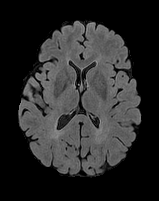
\includegraphics[width=\MRIwidth]{figures/MICCAI2015_CHB07-FLAIR-s88} &
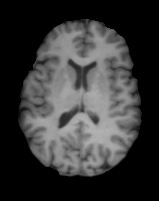
\includegraphics[width=\MRIwidth]{figures/MICCAI2015_CHB07-T1w-s88} &
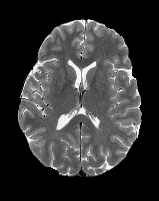
\includegraphics[width=\MRIwidth]{figures/MICCAI2015_CHB07-T2w-s88} &
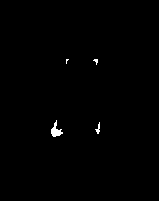
\includegraphics[width=\MRIwidth]{figures/MICCAI2015_CHB07-gold-s88} &
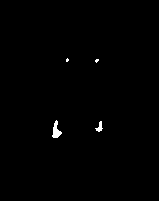
\includegraphics[width=\MRIwidth]{figures/MICCAI2015_CHB07-pred-s88} \\
\node[leftlabel] {CHB\,04\\(DSC\,=\,\SI{61.37}{\percent})}; &
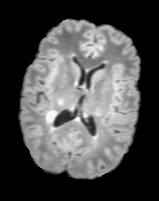
\includegraphics[width=\MRIwidth]{figures/MICCAI2015_CHB04-FLAIR-s85} &
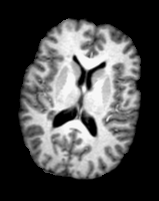
\includegraphics[width=\MRIwidth]{figures/MICCAI2015_CHB04-T1w-s85} &
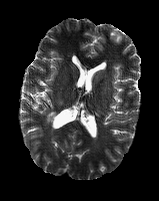
\includegraphics[width=\MRIwidth]{figures/MICCAI2015_CHB04-T2w-s85} &
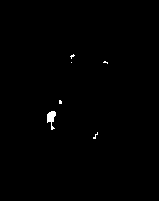
\includegraphics[width=\MRIwidth]{figures/MICCAI2015_CHB04-gold-s85} &

\includegraphics[width=\MRIwidth]{figures/MICCAI2015_CHB04-pred-s85} \\
\node[leftlabel] {UNC\,09\\(DSC\,=\,\SI{9.01}{\percent})}; &
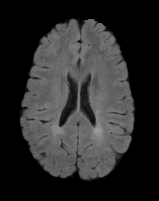
\includegraphics[width=\MRIwidth]{figures/MICCAI2015_UNC09-FLAIR-s89} &
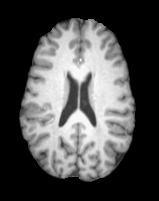
\includegraphics[width=\MRIwidth]{figures/MICCAI2015_UNC09-T1w-s89} &
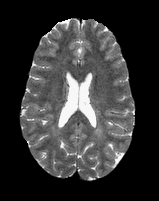
\includegraphics[width=\MRIwidth]{figures/MICCAI2015_UNC09-T2w-s89} &

\includegraphics[width=\MRIwidth]{figures/MICCAI2015_UNC09-gold-s89} &

\includegraphics[width=\MRIwidth]{figures/MICCAI2015_UNC09-pred-s89} \\
};
\end{tikzpicture}

\caption{Example segmentations of our method for three different subjects from
the challenge data set. Our method performed well and consistently despite the
large contrast differences seen between the first two rows. In the third row,
our method also segmented lesions that have similar contrast, but these regions
had not been identified as lesions by the manual rater, which highlights the
difficulty in distinguishing focal lesions from diffuse damage, even for
experts.}

\label{fig:segmentation}
\end{figure}

We evaluated our method on the challenge data set using 5-fold
cross-valida\-tion and calculated the true positive rate (TPR), positive
predictive value (PPV), and Dice similarity coefficient (DSC) between the
predicted segmentations and the resampled ground truth.
Figure~\ref{fig:segmentation} shows a comparison of three subjects from the
challenge data set. The first two rows show the FLAIR, T1w, T2w, ground truth
segmentations, and predicted segmentations of two subjects with a DSC of
\SI{60.58}{\percent} and \SI{61.37}{\percent}. Despite the large contrast
differences between the two subjects, our method performed well and
consistently, which indicates that our model was able to learn features that are
robust to a large range of intensity variations. The last row shows a subject
with a DSC of \SI{9.01}{\percent}, one of the lowest DSC scores from the data
set. Our method segmented lesions that have similar contrast to the other two
subjects, but these regions were not classified as lesions by the manual rater.
This highlights the difficulty of manual lesion segmentation, as the difference
between diffuse white matter pathology and focal lesions is often indistinct. A
quantitative comparison of our method with other state-of-the-art methods is
summarized in Table~\ref{tab:state}. Our method outperforms the winning method
(Souplet et al. \cite{souplet2008}) of the MS lesion segmentation challenge 2008
and the currently best unsupervised method reported on that data set (Weiss et
al. \cite{weiss2013}) in terms of mean TPR and PPV. Our method performs
comparably to a current method (Geremia et al. \cite{geremia2010}) that uses a
carefully designed set of features specifically designed for lesion
segmentation, despite our method having learned its features solely from a
relatively small training set.

\begin{table}[tb]
\def\tabspace{12pt}

\caption{Comparison of our method with state-of-the-art lesion segmentation
methods in terms of mean TPR, PPV, and DSC. Our method performs comparably to
the best methods reported on the MS lesion segmentation challenge data set.}

\label{tab:state}
\centering
\begin{tabular}{l%
@{\hspace{\tabspace}}S[table-format=2.2]
@{\hspace{\tabspace}}S[table-format=2.2]
@{\hspace{\tabspace}}S[table-format=2.2]
}
\toprule
Method & {TPR} & {PPV} & {DSC} \\ 
\midrule
Souplet et al. \cite{souplet2008} & 20.65 & 30.00 & {---} \\ 
Weiss et al. \cite{weiss2013} & 33.00 & 36.85 & 29.05 \\ 
Geremia et al. \cite{geremia2010} & 39.85 & 40.35 & {---}  \\
Our method & 39.71 & 41.38 & 35.52 \\
\bottomrule
\end{tabular}
\end{table}

To evaluate the impact of the training set size on the segmentation performance,
we trained our model on our in-house data set with a varying number of training
samples and calculated the mean DSC on the training and test sets as illustrated
in Fig.~\ref{fig:bioms}. For small training sets, there is a large difference
between the DSCs on the training and test sets, which indicates that the
training set is too small to learn a representative set of features. At around
100 samples, the model becomes stable in terms of test performance and the small
difference between training and test DSCs, indicating that overfitting of the
training data is no longer occurring. With 100 training subjects, our method
achieves a mean DSC on the test set of \SI{57.38}{\percent}, which shows that
the segmentation accuracy can be greatly improved compared to the results on the
challenge data set, when a representative training set is available.

\begin{figure}[tb]
\centering
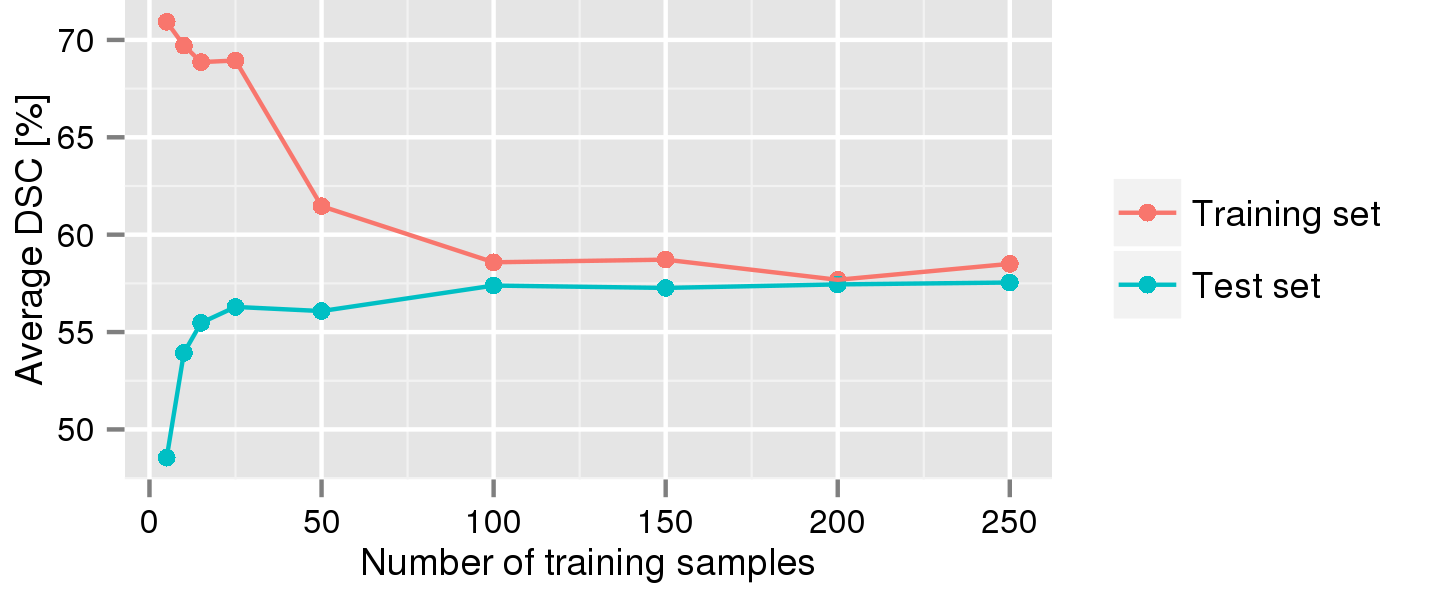
\includegraphics[width=0.78\textwidth]{figures/MICCAI2015_train_count}

\caption{Comparison of DSC scores calculated on the training and test sets for
varying numbers of training samples. At around 100 samples, the model becomes
stable in terms of test performance and the small difference between training
and test DSCs, indicating that overfitting of the training data no longer
occurs.}
\label{fig:bioms}
\end{figure}

\section{Evaluation on In-house Data}

We evaluated the proposed method on a large data set from a multi-center MS
clinical trial. The data set, acquired from 67 different scanning sites,
consists of 377 pairs of FLAIR and T1-weighted MRIs from 195 subjects with a
resolution of \num{256x256x60} voxels and a voxel size of
\SI{0.936x0.936x3.000}{\milli\metre}. All images were skull-stripped using the
brain extraction tool (BET) \cite{jenkinson2005bet2}, followed by an intensity
normalization to the interval $[0,1]$, and a 6 degrees-of-freedom intra-subject
registration. To speed-up the training, all images were cropped to a
\num{164x206x52} voxel region-of-interest with the brain roughly centered. The
ground truth segmentations were produced using an existing semiautomatic 2D
region-growing technique, which has been used successfully in a number of large
MS clinical trials (e.g., \cite{kappos2006long} and
\cite{traboulsee2008reduction}). To carry out the segmentation, each lesion was
manually identified by a trained technician and then interactively grown from
the seed point. We used 300 image pairs for pre-training and fine-tuning, and
the remaining 77 image pairs for evaluation. Pre-training and fine-tuning were
performed using highly optimized GPU-accelerated implementations of 3D convRBMs
and CENs that were developed in-house \cite{brosch2014efficient}. Each model was
trained using 500 epochs. Pre-training and fine-tuning of a 7-layer CEN-s took
approximately 27 hours and 37 hours, respectively, on a single GeForce GTX 780
graphics card. However, once the network is trained, new image pairs can be
segmented in less than one second. We compared our results to the lesion masks
produced by Lesion-TOADS \cite{shiee2010topology}, a widely used freely
available tool for the fully automatic segmentation of MS lesions.

\subsection{Measures of Segmentation Accuracy}

We have used three different measures to evaluate segmentation accuracy. The
primary measure of accuracy that we employ is the Dice similarity coefficient
(DSC) \cite{dice1945measures}, which computes a normalized overlap value between
the produced and ground truth segmentations, and is defined as
\begin{equation}
\text{DSC} = \frac{2 \times \text{TP}}{2 \times \text{TP} + \text{FP} +
\text{FN}},
\end{equation}
where TP, FP, and FN denote the number of true positives, false positives, and
false negatives, respectively. A value of \SI{100}{\percent} indicates a perfect
overlap of the produced segmentation and the ground truth.
The DSC incorporates measures of over- and undersegmentation into a single
metric, which makes it a suitable measure to compare overall segmentation
accuracy.
In addition, we have used the true positive rate (TPR) and the positive
predictive value (PPV) to provide further information on specific aspects of
segmentation performance. The TPR is used to measure the fraction of the lesion
regions in the ground truth that are correctly identified by
an automatic method. It is defined as
\begin{equation}
\text{TPR} = \frac{\text{TP}}{\text{TP} + \text{FN}},
\end{equation}
where a value of \SI{100}{\percent} indicates that all true lesion voxels are
correctly identified. The PPV is used to determine the extent of the regions
falsely classified as lesion by an automatic method. It is defined as the
fraction of true lesion voxels out of all identified lesion voxels
\begin{equation}
\text{PPV} = \frac{\text{TP}}{\text{TP} + \text{FP}},
\end{equation}
where a value of \SI{100}{\percent} indicates that all voxels that are
classified as lesion voxels are indeed lesion voxels as defined by the ground
truth.

\subsection{Comparison of Network Architectures}

To determine the effect of network architecture, we compared the segmentation
performance of three different networks with each other and with Lesion-TOADS.
Specifically, we trained a 3-layer CEN and two 7-layer CENs, one with shortcut
connections and one without, on the 300 training pairs. The parameters of the
networks are given in Table~\ref{tab:arch3} and Table~\ref{tab:arch7}.
A comparison of the segmentation accuracy of the trained networks and
Lesion-TOADS is summarized in Table~\ref{tab:results1}. All CEN architectures
performed significantly better than Lesion-TOADS in overall segmentation
accuracy, where the improvements of the mean DSC scores range from 9\,pts for
the 3-layer CEN to 14\,pts for the 7-layer CEN with shortcut connections. The
improved segmentation performance is mostly due to a reduction of the false
positives. Lesion-TOADS achieved a mean PPV of only \SI{39.86}{\percent},
whereas the CEN with shortcut achieved a mean PPV of \SI{66.58}{\percent}---an
improvement of 27\,pts. The mean TPRs were roughly the same (slightly less than
\SI{50}{\percent}) for all methods except for the 7-layer CEN with shortcut,
which performed slightly better than the other methods with a mean TPR of
\SI{52.75}{\percent}.

Furthermore, the first experiment showed that increasing the depth of the CEN
and adding the shortcut connections improves the segmentation accuracy.
Increasing the depth of the CEN from three layers to seven layers improved the
mean DSC by 2\,pts. The improvement was confirmed to be statistically
significant using a one-sided paired $t$-test ($p\text{-value}=\num{0.002}$).
Adding a shortcut to the network further improved the segmentation
accuracy as measured by the DSC by 3\,pts. A second one-sided paired $t$-test
was performed to confirm the statistical significance of the improvement with a
$p$-value of \num{1.566e-11}.

% \begin{itemize}
% \item We used 3 different architectures: 3-layer, 7-layer without shortcuts and
% 7-layer with shortcuts.
% \item 7-layer CEN parameters are summarized in Table~\ref{tab:arch7}.
% \item Comparison of segmentation performance on the test set with 3 different
% architectures and lesionTOADS is shown in Table~\ref{tab:results1}
% \item Even the 3-layer model performs much better than lesionTOADS on average.
% \item Better was confirmed using a one-sided paired t-test. Give the p-value.
% \item Better than lesionTOADS ($p$-value = \num{4.732e-9})
% \item Better than 3-layer ($p$-value = \num{0.002})
% \item Better with shortcut connections ($p$-value = \num{1.566e-11})
% \item Adding more layers also improves performance. T-test.
% \item Adding shortcut connections improves performance. t-test.
% \end{itemize}

\begin{table}[tb]
\caption{Parameters of the 3-layer CEN used to evaluate different training
methods.}
\label{tab:arch3}
\centering
\begin{tabular}{@{}lccr@{}}
\toprule
Layer type & Kernel Size & \#Filters & \multicolumn{1}{c}{Image Size} \\
\midrule
Input & --- & --- & \num{164x206x52x2}\phantom{0} \\
Convolutional & \num{9x9x5x2} & 32 & \num{156x198x48x32} \\
Deconvolutional & \num{9x9x5x32} & 1 & \num{164x206x52x1}\phantom{0} \\
\bottomrule
\end{tabular}
\end{table}

\begin{table}[tb]
\caption{Parameters of the 7-layer CEN-s used to evaluate different training
methods.}
\label{tab:arch7}
\centering
\begin{tabular}{@{}lccr@{}}
\toprule
Layer type & Kernel Size & \#Filters & \multicolumn{1}{c}{Image Size} \\
\midrule
Input & --- & --- & \num{164x206x52x2}\phantom{0} \\
Convolutional & \num{9x9x5x2} & 32 & \num{156x198x48x32} \\
Average Pooling & \num{2x2x2} & --- & \num{78x99x24x32} \\
Convolutional & \num{9x10x5x32} & 32 & \num{70x90x20x32} \\
Deconvolutional & \num{9x10x5x32} & 32 & \num{78x99x24x32} \\
Unpooling & \num{2x2x2} & --- & \num{156x198x48x32} \\
Deconvolutional & \num{9x9x5x32} & 1 & \num{164x206x52x1}\phantom{0} \\
\bottomrule
\end{tabular}
\end{table}

\begin{table}
\begin{center}
\caption{Comparison of the segmentation accuracy of different CEN models with
Lesion-TOADS}
\label{tab:results1}
\begin{tabular}{@{}lccc@{}}
\toprule
Method & TPR [\%] & PPV [\%] & DSC [\%] \\
\midrule
3-layer CEN \cite{brosch2015} & \num{49.62+-20.32} & \num{59.87+-20.95} &
\num{49.1+-15.78} \\
7-layer CEN & \num{49.94+-19.96} & \num{63.5+-20} & \num{51.04+-14.71} \\
7-layer CEN-s & \num{52.75+-20.31} & \num{66.58+-20.71} &
\num{54.02+-15.24}
\\[0.2em]
Lesion-TOADS \cite{shiee2010topology} & \num{49.83+-14.79} & \num{39.86+-20.95} &
\num{40.04+-14.86} \\
\bottomrule
\end{tabular}
\end{center}
Note: The table shows the mean and standard deviation of the true positive rate
(TPR), positive predictive value (PPV), and Dice similarity coefficient (DSC).
\end{table}

\subsection{Comparison for Different Lesion Loads}

To examine the effect of lesion load on segmentation performance, we have
stratified the test set into five groups based on their reference lesion loads
as summarized in Table~\ref{tab:groups}. Most segmentation performance measures
deteriorate with lower lesion loads, because when there are only a few true
lesion voxels, even small segmentation errors can translate into large relative
errors. A comparison of segmentation accuracy of a 3-layer CEN and a 7-layer CEN
with shortcut for different lesion loads is illustrated in
Fig.~\ref{fig:l1vl2}. Adding four layers and shortcut connections improves the
segmentation accuracy for all lesion load groups, where the improvements are
largest for the highest lesion loads. In MS, lesion load is strongly
correlated with lesion size, which means that the group with the highest lesion
load also contains scans with the largest lesions. The receptive field of the
3-layer CEN has a size of only \num{17x17x9} voxels, which reduces its ability
to identify very large lesions. In contrast, the 7-layer CEN has a receptive
field size of \num{49x53x26} voxels, which allows it to learn features that can
capture much larger lesions than the 3-layer CEN. Consequently, the 7-layer CEN
is able to learn a feature set that captures a wider range of lesion sizes,
which in turn improves the segmentation accuracy especially for very high lesion
loads, where larger lesions are also more prevalent.

\begin{table}[tb]
\caption{Lesion load classes as used for the detailed analysis.}
\label{tab:groups}
\centering
\begin{tabular}{@{}lcc@{}}
\toprule
Group & Lesion load in \si{\cubic\milli\metre} & Number of samples \\
\midrule
% 0, 1250, 2500, 3800, 10000
Very low & $[0,3250]$ & 17 \\
Low      & $(3250,6500]$ & 16 \\
Medium & $(6500,10000]$ & 18 \\
High & $(10000,25000]$ & 18 \\
Very high & $> 25000$ & 8 \\
\bottomrule
\end{tabular}
\end{table}

% \begin{itemize}
% \item Analyse where the performance gains come from
% \item 7-layer CEN improves across the board but improvements are particularly
% high for large lesion loads
% \item Large lesion load is also associated with larger lesions
% \item Small filters fail to detect large lesions correctly
% \item 7-layer CEN uses a hierachy of features where each layer represents
% features of a different scale
% \item This allows the detection of a wider spectrum of lesion sizes.
% \item Analyse the relationship of segmentation performance and lesion load
% \item Divided the test set into 5 classes with roughly the same number of
% samples. Classes are (0,1250) ($n=17$), (1250,2500) ($n=16$), (2500, 3800)
% ($n=18$), (3800,10000) ($n=18$), above 10000 ($n=8$). Mention the number of
% samples per class.
% \item CEN outperforms Lesion-TOADS for all lesion load categories, except for
% very high lesion load.
% \item For very high lesion load, no difference to Lesion-TOADS found using
% t-test.
% \item TPR, PPV, DSC for different lesion loads in a table.
% \end{itemize}

\begin{figure}[tb]
\centering
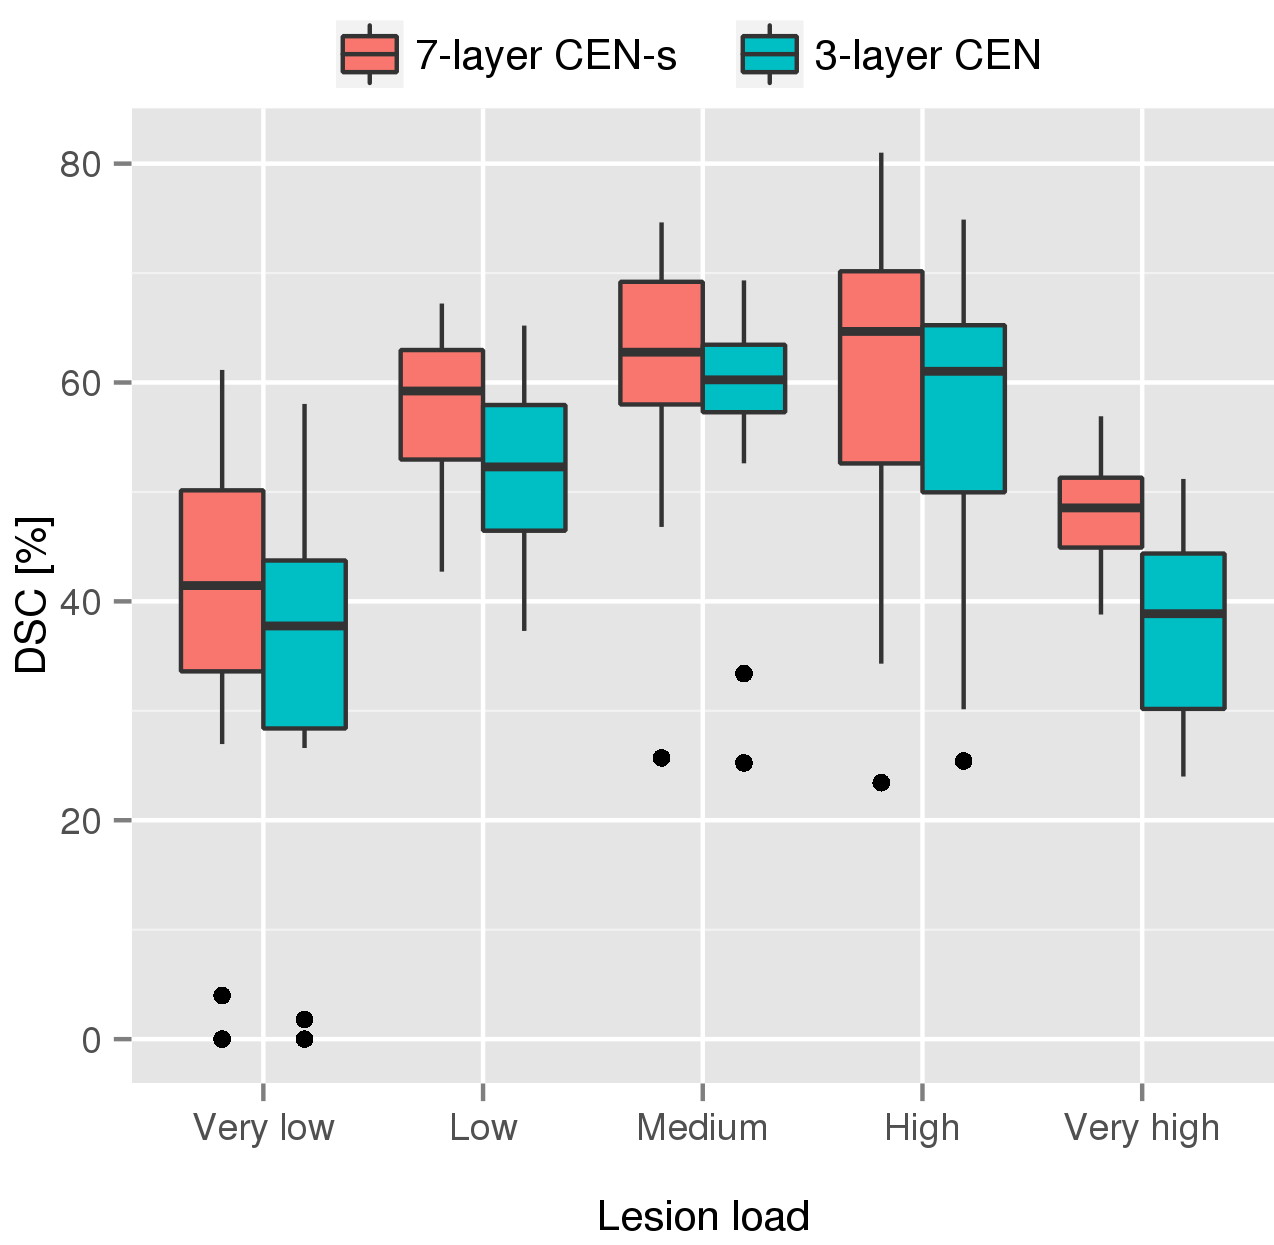
\includegraphics[width=\columnwidth]{figures/TMI_boxplot_L1vsL2}

\caption{Comparison of the segmentation accuracy (DSC) of a 3-layer CEN and a
7-layer CEN-s for different lesion load groups. Adding four layers and
shortcut connections improves the performance across all lesion loads, where the
improvements are especially large for scans with large lesion loads, which are
also correlated with lesion size.}

\label{fig:l1vl2}
\end{figure}

% TODO: The small number of scans in the highest load group makes comparing
% across groups difficult. Maybe weaken the statement or point out the
% limitation with sample size.

Fig.~\ref{fig:l2vlt} shows a comparison of the 7-layer CEN with shortcut and
Lesion-TOADS. The CEN approach performs more consistently than Lesion-TOADS for
all lesion load groups, but the greatest improvements are for very low to medium
lesion loads. For the group with very high lesion loads, Lesion-TOADS achieves a
slightly higher mean DSC than the CEN approach, but the difference is very small
compared to the gains in accuracy achieved by the CEN for the other lesion load
groups.
% However, a two-sided paired $t$-test yielded that
% the difference is not statistically significant ($p\text{-value}=0.2566$).
Table~\ref{tab:result2} shows a more detailed
comparison. While the PPV increases consistently with higher lesion loads for
both methods, the TPR is highest for low to medium lesion loads and decreases
again for high to very high lesion loads. This shows the difficulty for both
methods to correctly identify very large lesions that can extend far into the
white matter.

\begin{figure}[tb] \centering
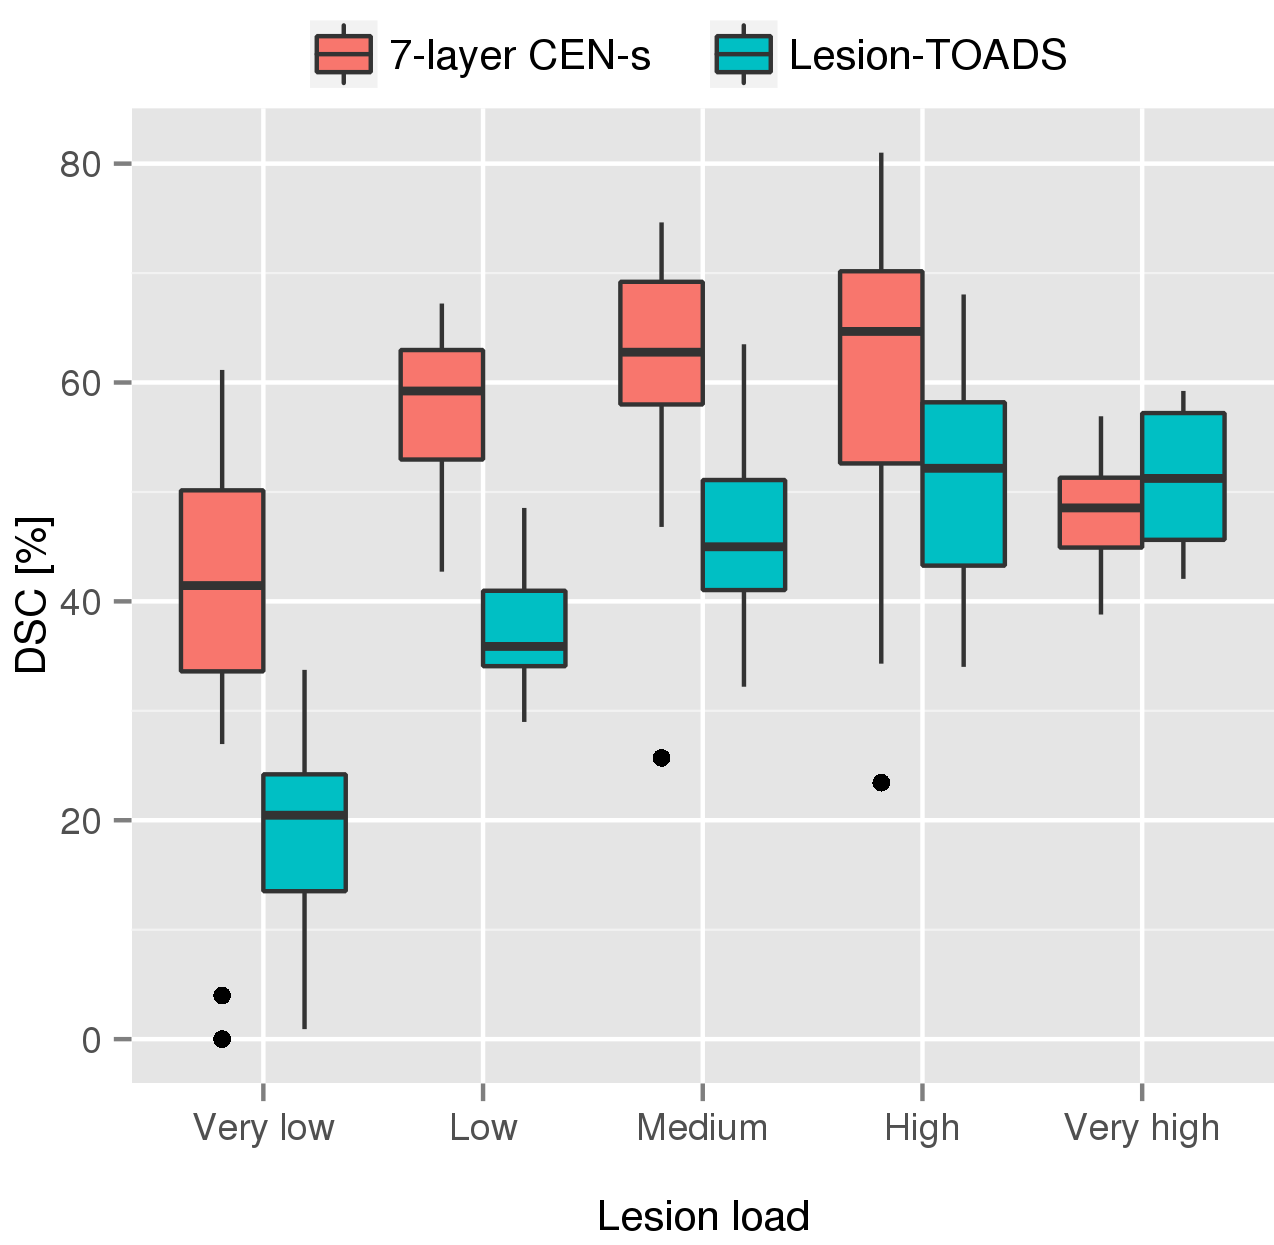
\includegraphics[width=\columnwidth]{figures/TMI_boxplot_LTvsL2}
\caption{Comparison of the segmentation accuracy (DSC) of
Lesion-TOADS and a 7-layer CEN with shortcut connections for different lesion
loads. The CEN approach is much more sensitive in detecting small lesions, while
still being able to detect large lesions.}
\label{fig:l2vlt}
\end{figure}

\begin{table}
\caption{Comparison of segmentation accuracy for different lesion load
categories.}
\label{tab:result2}
\begin{center}
\begin{tabular}{@{}lcccccc@{}}
\toprule
\multicolumn{1}{@{}l}{Lesion load} & \multicolumn{3}{c}{7-layer CEN-s} &
\multicolumn{3}{c@{}}{Lesion-TOADS}
\\
& TPR & PPV & DSC & TPR & PPV & DSC \\
\midrule
% \phantom{000}$(0,1250]$\phantom{0} & \num{50.00} & \num{41.15} & \num{39.34} &
% \num{49.96} & \num{13.09} & \num{18.86}\\
% $(1250,2500]$\phantom{0} & \num{61.92} & \num{59.01} & \num{57.45} & \num{52.39}
% & \num{29.95} & \num{37.74}\\
% $(2500,3800]$\phantom{0} & \num{57.64} & \num{71.54} & \num{61.31} & \num{54.17}
% & \num{41.83} & \num{46.53}\\
% $(3800,10000]$ & \num{51.14} & \num{81.11} & \num{60.13} & \num{47.97} &
% \num{56.56} & \num{50.76}\\
% $> 10000$ & \num{32.82} & \num{91.95} & \num{48.19} & \num{38.88} & \num{74.6} &
% \num{50.93}\\
Very low & \num{50.00} & \num{41.15} & \num{39.34} &
\num{49.96} & \num{13.09} & \num{18.86}\\
Low & \num{61.92} & \num{59.01} & \num{57.45} & \num{52.39}
& \num{29.95} & \num{37.74}\\
Medium & \num{57.64} & \num{71.54} & \num{61.31} & \num{54.17}
& \num{41.83} & \num{46.53}\\
High & \num{51.14} & \num{81.11} & \num{60.13} & \num{47.97} &
\num{56.56} & \num{50.76}\\
Very high & \num{32.82} & \num{91.95} & \num{48.19} & \num{38.88} & \num{74.6} &
\num{50.93}\\
\bottomrule
\end{tabular}
\end{center}
\end{table}

% \begin{itemize}
% \item Have some sample images and discuss what we can see here.
% \end{itemize}

\subsection{Qualitative Results}

A qualitative comparison of segmentation performance for four characteristic
cases is shown in Fig.~\ref{fig:images}. Our method uses a combination of
automatically learned intensity and appearance features, which makes it
inherently robust to noise (see Fig.~\ref{fig:images}a), while still being able
to detect small isolated lesions (see Fig.~\ref{fig:images}b). Furthermore, our
method is able to learn a wide spectrum of lesion shapes and appearances from
training data, which allows our method to correctly identify multiple different
types of MS lesions. For example, our method was able to correctly identify the
T1 black hole shown in Fig.~\ref{fig:images}c, which present a known limitations
of Lesion-TOADS \citep{shiee2010} and was partially missed.
Figure~\ref{fig:images}d shows one of the most challenging cases for our method.
Very large lesions can extend beyond the size of the receptive field of the CEN,
which reduces its ability to extract characteristic lesion features.
Consequently, in some cases our method can underestimate the size of very large
lesions.

\begin{figure}
%\centering
\hspace*{-5pt}
\subfloat[Robust to noise] {
\begin{tikzpicture}[node distance=1.5cm and 0.1\columnwidth,
  font=\footnotesize, on grid]
  
\node[inner sep=0] (image) {
  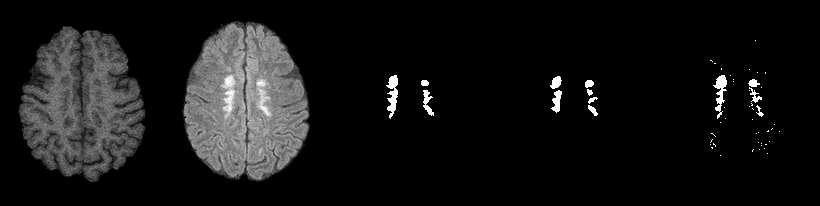
\includegraphics[width=0.5\columnwidth]{figures/TMI_p15s34_robust_to_noise3}
  }; \node[above=of image] (gt) {\phantom{g}Ground truth\phantom{g}};
\node[left=of gt] (flair) {\phantom{g}FLAIR\phantom{g}};
\node[left=of flair] {T1-weighted};
\node[right=of gt,align=center] (cen) {\phantom{g}Our method\phantom{g}};
\node[right=of cen,align=center] {Lesion-\\ TOADS};


\end{tikzpicture}
}
\subfloat[Can detect small isolated lesions.] {
\begin{tikzpicture}[node distance=1.5cm and 0.1\columnwidth,
  font=\footnotesize, on grid]
  
\node[inner sep=0] (image) {
  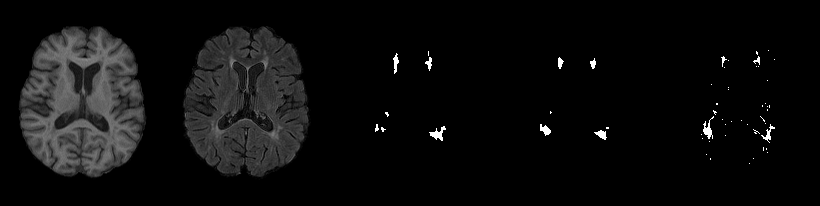
\includegraphics[width=0.5\columnwidth]{figures/TMI_p17s29_noisy_lesionTOADS}};
  \node[above=of image] (gt) {\phantom{g}Ground truth\phantom{g}};
\node[left=of gt] (flair) {\phantom{g}FLAIR\phantom{g}};
\node[left=of flair] {T1-weighted};
\node[right=of gt,align=center] (cen) {\phantom{g}Our method\phantom{g}};
\node[right=of cen,align=center] {Lesion-\\ TOADS};

\draw[green, thick] (-7pt,-3.5pt) circle (3pt);
\begin{scope}[xshift=0.1\columnwidth]
\draw[green, thick] (-7pt,-3.5pt) circle (3pt);
\end{scope}

\end{tikzpicture}
}\\
\hspace*{-5pt}
\subfloat[Example of a T1 black hole that was correctly identified by our
method.] {
\begin{tikzpicture}
\node[inner sep=0pt] {
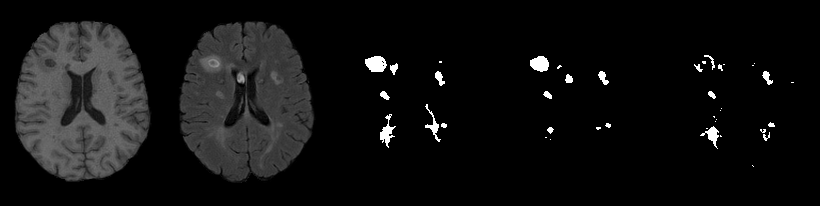
\includegraphics[width=0.5\columnwidth]{figures/TMI_p36s30_blackhole}};
\draw[red,thick] (-10pt,12pt) circle (7pt);
\begin{scope}[xshift=-0.1\columnwidth]
\draw[red,thick] (-10pt,12pt) circle (7pt);
\end{scope}
\begin{scope}[xshift=-0.2\columnwidth]
\draw[red,thick] (-10pt,12pt) circle (7pt);
\end{scope}
\begin{scope}[xshift=0.1\columnwidth]
\draw[red,thick] (-10pt,12pt) circle (7pt);
\end{scope}
\begin{scope}[xshift=0.2\columnwidth]
\draw[red,thick] (-10pt,12pt) circle (7pt);
\end{scope}
\end{tikzpicture}
}
\subfloat[Very large lesions can be underestimated] {
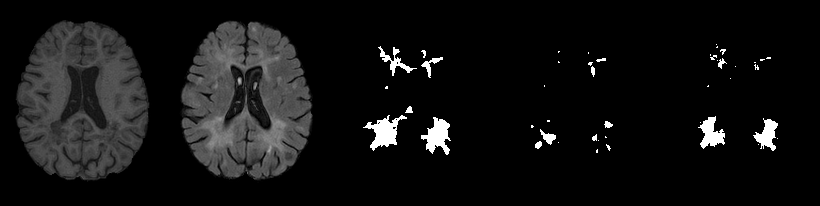
\includegraphics[width=0.5\columnwidth]{figures/TMI_p54s32_large_lesions}
}

\caption{Four cases illustrating the strengths and limitations of our method
compared to Lesion-TOADS. Our method is inherently robust to noise (a), while
still being able to detect small isolated lesions (b). Furthermore, our method
is able to detect multiple different types of lesions correctly (e.g.,
T1 black holes). However, in some cases our method can underestimate the size
of very large lesions (d).}

\label{fig:images}
\end{figure}

\chapter{Discussion}

What else do I need? General discussion of the role of deep learning for medical
image analysis. Maybe.

\chapter{Future Work}

Future work: different models like RNNs, LSTMs. Learning
invariance to rotations might help especially in 3D. What are other
applications? Also need to understand models better. Visualize them maybe?
Better training algorithms? More data? Better regularization?

\chapter{Conclusion}

Important field and great potential.


\singlespacing
% \nocite{*}
\bibliography{bibliography/newbib}

%\appendix

%\include{chapters/A_gpudetails}

\end{document}
